%% This is file `elsarticle-template-1-num.tex',
%%
%% Copyright 2009 Elsevier Ltd
%%
%% This file is part of the 'Elsarticle Bundle'.
%% ---------------------------------------------
%%
%% It may be distributed under the conditions of the LaTeX Project Public
%% License, either version 1.2 of this license or (at your option) any
%% later version.  The latest version of this license is in
%%    http://www.latex-project.org/lppl.txt
%% and version 1.2 or later is part of all distributions of LaTeX
%% version 1999/12/01 or later.
%%
%% The list of all files belonging to the 'Elsarticle Bundle' is
%% given in the file `manifest.txt'.
%%
%% Template article for Elsevier's document class `elsarticle'
%% with numbered style bibliographic references
%%
%% $Id: elsarticle-template-1-num.tex 149 2009-10-08 05:01:15Z rishi $
%% $URL: http://lenova.river-valley.com/svn/elsbst/trunk/elsarticle-template-1-num.tex $
%%
\documentclass[preprint,12pt]{elsarticle}

%% Use the option review to obtain double line spacing
%% \documentclass[preprint,review,12pt]{elsarticle}

%% Use the options 1p,twocolumn; 3p; 3p,twocolumn; 5p; or 5p,twocolumn
%% for a journal layout:
%% \documentclass[final,1p,times]{elsarticle}
%% \documentclass[final,1p,times,twocolumn]{elsarticle}
%% \documentclass[final,3p,times]{elsarticle}
%% \documentclass[final,3p,times,twocolumn]{elsarticle}
%% \documentclass[final,5p,times]{elsarticle}
%% \documentclass[final,5p,times,twocolumn]{elsarticle}

%% if you use PostScript figures in your article
%% use the graphics package for simple commands
%% \usepackage{graphics}
%% or use the graphicx package for more complicated commands
%% \usepackage{graphicx}
%% or use the epsfig package if you prefer to use the old commands
%% \usepackage{epsfig}

%% The amssymb package provides various useful mathematical symbols
\usepackage{graphicx}
\usepackage{amssymb}
\setcounter{tocdepth}{3}
\usepackage{amsmath}
\usepackage{amssymb}
\usepackage{color}
\usepackage{tikz}
\usepackage{pgfplots}
\usepackage{caption}
\usepackage{subcaption}
\usepackage{comment}
\usepackage{booktabs}
\usepackage{nopageno}
\usepackage{sidecap}

\usepackage[algo2e, noend, noline, linesnumbered]{algorithm2e}
%\DontPrintSemicolon
\providecommand{\SetAlgoLined}{\SetLine}
\providecommand{\DontPrintSemicolon}{\dontprintsemicolon}
\DontPrintSemicolon
\makeatletter
\newcommand{\pushline}{\Indp}% Indent
\newcommand{\popline}{\Indm}
\makeatother
\DeclareMathOperator{\pess}{pess}
\DeclareMathOperator{\opti}{opti}
\newcommand{\argmax}{\operatornamewithlimits{argmax}}

\captionsetup{compatibility=false}



%\pgfplotsset{compat=newest}
\usetikzlibrary{arrows,shapes,petri}

\newcommand{\bE}{\mathbb{E}}
\newcommand{\cA}{\mathcal{A}}
\newcommand{\cC}{\mathcal{C}}
\newcommand{\cD}{\mathcal{D}}
\newcommand{\cI}{\mathcal{I}}
\newcommand{\cH}{\mathcal{H}}
\newcommand{\cN}{\mathcal{N}}
\newcommand{\cO}{\mathcal{O}}
\newcommand{\cP}{\mathcal{P}}
\newcommand{\cS}{\mathcal{S}}
\newcommand{\cT}{\mathcal{T}}
\newcommand{\cZ}{\mathcal{Z}}
\newcommand{\bVar}{\mathbf{Var}}
\newcommand{\bCov}{\mathbf{Cov}}
\newcommand{\eg}{{e.g.,}~}
\newcommand{\ie}{{i.e.,}~}
\newcommand{\defword}[1]{\textbf{\boldmath{#1}}}
\newcommand{\reviewchange}[1]{{\color{black}#1}}
\newcommand{\reviewchangeT}[1]{{\color{black}#1}}

\definecolor{darkgreen}{RGB}{0,125,0}
\newcounter{mwNoteCounter}
\newcounter{mlNoteCounter}
\newcounter{vlNoteCounter}
\newcounter{bbNoteCounter}
\newcounter{jcNoteCounter}
\newcommand{\mwinands}[1]{{\small \color{blue} $\blacksquare$ \refstepcounter{mwNoteCounter}\textsf{[RGG]$_{\arabic{mwNoteCounter}}$:{#1}}}}
\newcommand{\mlanctot}[1]{{\small \color{darkgreen} $\blacksquare$ \refstepcounter{mlNoteCounter}\textsf{[ML]$_{\arabic{mlNoteCounter}}$:{#1}}}}
\newcommand{\vlisy}[1]{{\small \color{red} $\blacktriangle$ \refstepcounter{vlNoteCounter}\textsf{[VL]$_{\arabic{vlNoteCounter}}$:{#1}}}}
\newcommand{\bbosansky}[1]{{\small \color{orange} $\blacktriangle$ \refstepcounter{bbNoteCounter}\textsf{[BB]$_{\arabic{bbNoteCounter}}$:{#1}}}}
\newcommand{\jcermak}[1]{{\small \color{violet} $\blacktriangle$ \refstepcounter{jcNoteCounter}\textsf{[JC]$_{\arabic{jcNoteCounter}}$:{#1}}}}
\renewcommand{\mwinands}[1]{}
%\renewcommand{\mlanctot}[1]{}
%\renewcommand{\vlisy}[1]{}
%\renewcommand{\bbosansky}[1]{}
\renewcommand{\jcermak}[1]{}


\newtheorem{theorem}{Theorem}[section]
\newtheorem{lemma}[theorem]{Lemma}
\newtheorem{proposition}[theorem]{Proposition}
\newtheorem{corollary}[theorem]{Corollary}
\newtheorem{definition}[theorem]{Definition}

\newenvironment{proof}[1][Proof]{\begin{trivlist}
\item[\hskip \labelsep {\bfseries #1}]}{\end{trivlist}}

\newcommand{\doab}[0]{\textrm{DO}\alpha\beta}
\newcommand{\biab}[0]{\textrm{BI}\alpha\beta}
\newcommand{\bdoab}[0]{\textrm{\bf DO}\boldsymbol{\alpha\beta}}
\newcommand{\bbiab}[0]{\textrm{\bf BI}\boldsymbol{\alpha\beta}}


%% The amsthm package provides extended theorem environments
%% \usepackage{amsthm}

%% The lineno packages adds line numbers. Start line numbering with
%% \begin{linenumbers}, end it with \end{linenumbers}. Or switch it on
%% for the whole article with \linenumbers after \end{frontmatter}.
%% \usepackage{lineno}

%% natbib.sty is loaded by default. However, natbib options can be
%% provided with \biboptions{...} command. Following options are
%% valid:

%%   round  -  round parentheses are used (default)
%%   square -  square brackets are used   [option]
%%   curly  -  curly braces are used      {option}
%%   angle  -  angle brackets are used    <option>
%%   semicolon  -  multiple citations separated by semi-colon
%%   colon  - same as semicolon, an earlier confusion
%%   comma  -  separated by comma
%%   numbers-  selects numerical citations
%%   super  -  numerical citations as superscripts
%%   sort   -  sorts multiple citations according to order in ref. list
%%   sort&compress   -  like sort, but also compresses numerical citations
%%   compress - compresses without sorting
%%
%% \biboptions{comma,round}

% \biboptions{}

\pagenumbering{arabic}
\journal{Artificial Intelligence}

\begin{document}

\begin{frontmatter}

%% Title, authors and addresses

%% use the tnoteref command within \title for footnotes;
%% use the tnotetext command for the associated footnote;
%% use the fnref command within \author or \address for footnotes;
%% use the fntext command for the associated footnote;
%% use the corref command within \author for corresponding author footnotes;
%% use the cortext command for the associated footnote;
%% use the ead command for the email address,
%% and the form \ead[url] for the home page:
%%
%% \title{Title\tnoteref{label1}}
%% \tnotetext[label1]{}
%% \author{Name\corref{cor1}\fnref{label2}}
%% \ead{email address}
%% \ead[url]{home page}
%% \fntext[label2]{}
%% \cortext[cor1]{}
%% \address{Address\fnref{label3}}
%% \fntext[label3]{}

\title{Algorithms for Computing Strategies in Two-Player Simultaneous Move Games}
% Offline and Online Strategy Computation in Zero-Sum Simultaneous Move Games

%% use optional labels to link authors explicitly to addresses:
%% \author[label1,label2]{<author name>}
%% \address[label1]{<address>}
%% \address[label2]{<address>}

\author[1]{Branislav Bo{\v s}ansk{\' y}$^1$}%\footnote{Corresponding author; phone: +420 22435 7581}}
\author[1]{Viliam Lis\'{y}}
\author[2]{Marc Lanctot$^2$}
\author[1]{Ji{\v r}{\' i} {\v C}erm{\' a}k}
\author[2]{\\Mark H.M. Winands}
\address[1]{Agent Technology Center, Department of Computer Science,\\ Faculty of Electrical Engineering, Czech Technical University in Prague\\
Technicka 2, 166 27 Prague 6, Czech Republic\\
\{branislav.bosansky,viliam.lisy,jiri.cermak\}@agents.fel.cvut.cz\\
$^1$Corresponding author; phone: +420 22435 7581
}
\address[2]{Games and AI Group, Department of Data Science and Knowledge Engineering, Maastricht University, \\P.O. Box 616, 6200 MD, Maastricht, The Netherlands\\
\{marc.lanctot,m.winands\}@maastrichtuniversity.nl\vspace{-0.5cm}}

%\footenotemark{This author has a new affiliation: Google DeepMind, London, United Kingdom.}


%Author list (+ corresponding author), affiliations, and contact info
%needed\footnote{\mlanctot{A lot of information is required on this title page... see AIJ guidelines}}}

%\address{}
\begin{abstract}
% TODO for final print, leave affiliation as Maastricht University but leave footnote for Marc:
\footnotetext[2]{This author has a new affiliation: Google DeepMind, London, United Kingdom.}

Simultaneous move games model discrete, multistage interactions where at each stage players simultaneously choose their actions.
\reviewchangeT{At each stage, a player does not know what action the other player will take, but otherwise knows the full state of the game.}
\reviewchange{
This formalism has been used to express games in general game playing and can also model many discrete approximations of real-world scenarios.
In this paper, we describe both novel and existing algorithms that compute strategies for the class of two-player zero-sum simultaneous move games.}
The algorithms include exact backward induction methods with efficient pruning, as well as Monte Carlo sampling algorithms.
We evaluate the algorithms in two different settings: the offline case, where computational
resources are abundant and closely approximating the optimal strategy is a priority, and
the online search case, where computational resources are limited and acting quickly is necessary.
We perform a thorough experimental evaluation on six substantially different games for both settings.
\reviewchange{
For the exact algorithms, the results show that our pruning techniques for backward induction dramatically improve the computation time required by the previous exact algorithms.
For the sampling algorithms, the results provide unique insights into their performance and identify favorable settings and domains for different sampling algorithms.
}

%Thorough experimental evaluation in six substantially different games shows that augmenting Backward Induction with a double oracle
%method and serialized bounds can compute an exact optimal strategy in less than 2\% of the time required by previous algorithms.
%% MarcL: I struggled a bit trying to summarize the results below, so please fix as needed.
%When used in online search, this method can match or out-perform the Monte Carlo algorithms when an accurate short-term assessment
%is needed, the overhead of sampling is significant, or the game has high support.
%For the Monte Carlo sampling algorithms, UCT can often find a good pure strategy quickly if one exixts, but in other games its
%recommendation can become consistently worse over time, diverging away from the optimal choice.
%In games where mixing among strategies is important, strategies built on regret matching perform well and are generally
%more robust to changes in parameter settings.
% Seems a bit too strong, now.
%   Furthermore, a new sampling algorithm
%   based on regret matching, dominates in the head-to-head tournament compared to
%   existing methods.
\end{abstract}

\begin{keyword}
%% keywords here, in the form: keyword \sep keyword
simultaneous move games \sep Markov games \sep backward induction \sep Monte Carlo Tree Search \sep alpha-beta pruning \sep double-oracle algorithm \sep regret matching \sep counterfactual regret minimization \sep game playing \sep Nash equilibrium

%% MSC codes here, in the form: \MSC code \sep code
%% or \MSC[2008] code \sep code (2000 is the default)
\end{keyword}

\end{frontmatter}

%%
%% Start line numbering here if you want
%%
% \linenumbers
%% The Appendices part is started with the command \appendix;
%% appendix sections are then done as normal sections
%% \appendix

%% \section{}
%% \label{}

%% References
%%
%% Following citation commands can be used in the body text:
%% Usage of \cite is as follows:
%%   \cite{key}          ==>>  [#]
%%   \cite[chap. 2]{key} ==>>  [#, chap. 2]
%%   \citet{key}         ==>>  Author [#]

%% References with bibTeX database:

%% main text
\section{Introduction}
\label{sec:intro}
%\bbosansky{unify subgame/sub-game; subfigure/sub-figure; etc.}
%\mlanctot{Ok, I'll do this on my full pass this week.}
% Done.

Strategic decision-making in multiagent environments is an important problem in artificial intelligence.
With the growing number of agents interacting with humans and with each other, the need to
understand these strategic interactions at a fundamental level is becoming increasingly important.
Today, agent interactions occur in many diverse situations, such as e-commerce, social networking, and
general-purpose robotics, each of which creates complex problems that arise from conflicting agent
preferences.

Much research has been devoted to developing algorithms that reason about or learn in sequential (multi-step)
interactions. As an example, adversarial search has been a central topic of artificial intelligence
since the inception of the field itself, leading to very strong rational behaviors in
Chess~\cite{Campbell02deepblue} and Checkers~\cite{Schaeffer96chinook}. Advances in machine learning for multi-step interactions
(\eg reinforcement learning) have led to self-play learning of evaluation functions achieving master level play
in Backgammon~\cite{Tesauro95TDGammon} and super-human level in Atari~\cite{mnih-dqn-2015}.

The most common model for these multistage environments is one with strictly sequential
interactions. 
%That is, each player chooses an action when it is their turn to act, then the environment 
%generates a new state, and the process continues.
This model is sufficient in many
settings~\cite{AIbook}, such as in the examples used above.
\reviewchange{On the other hand, it is not a good representation of the environment when agents are allowed to act simultaneously.
These situations occur in many real-world scenarios such as auctions~(\eg~\cite{Keuter1997}), autonomous driving, and many video
and board games in the expanding gaming industry (\eg~\cite{Beard12Using,Teytaud11Upper}, including games we use for our experiments).
In all of these scenarios, the simultaneity of the decision-making is crucial and we have to include it directly into the model when computing strategies.}
One of the fundamental differences of simultaneous move games versus strictly sequential
games is that the agents may need to use randomized (or \textit{mixed}) strategies in order to
play optimally~\cite{Gintis09},
\ie to maximize their worst-case expected utility.
\reviewchangeT{This means that agents may need to randomize over several actions in some states of the game
to guarantee the worst-case expected utility, even though the only information that is hidden is each player's
action as they play it.} %Chosen actions are revealed publically by each player after they have been played.
%Unless some information is hidden, this does not occur in strictly sequential games, where optimal
%solution always exists in deterministic (or \textit{pure}) strategies.

\reviewchange{This paper focuses specifically on algorithms for decision-making in simultaneous move games.} 
We cover the offline case, where the computation time is abundant and the optimal strategies are computed and stored, 
as well as the online case, where the computation time is limited and agents must choose an action quickly.
We are concerned both with the quality of strategies based on
their worst-case expected performance in theory and their observed performance in practice. 
We compare and contrast the algorithms and parameter choices in the offline and the online cases, and thoroughly evaluate each
algorithm on a suite of games. Our collection covers Biased Rock-Paper-Scissors, Goofspiel, Oshi-Zumo,
Pursuit-Evasion Games, and Tron, all of which have been used for benchmark purposes
in previous work. We also perform experiments on randomly generated games. These games differ
in the number of possible actions, the number of moves before the game ends, the variance of the utility values,
and the proportion of states in which mixed strategies are required for optimal play. % required for optimal play.

Our experimental comparison shows that the algorithms perform differently in each case.
\reviewchange{The exact algorithms based on the backward induction are significantly better in the offline setting,
where they are able to find the optimal strategy very quickly compared to the sampling algorithms.}
In some cases, our novel algorithm ($\doab$) solves the game in less than 2\% of the time required by the standard backward induction algorithm.
However, the exact algorithms are less competitive in the online setting.
In contrast, the approximative sampling algorithms can perform very well in the online setting and
find good strategies to play within a few seconds, however, they are not well-suited for offline solving of games.

The paper is structured as follows. \reviewchange{First, we make explicit the contributions of the paper in Subsection~\ref{sec:contrib}.}
In Section~\ref{sec:smg}, we present a formal introduction of the simultaneous move games that we will use throughout the paper.
Section~\ref{sec:relwork} follows with a list and discussion of the existing algorithms in the related work. In
Section~\ref{sec:offline}, we describe in detail selected exact and approximative algorithms.
We first describe the algorithms in the offline setting, followed by the necessary modifications used in the online
case described in Section~\ref{sec:online}.
%\reviewchange{In Section~\ref{sec:theory}, we discuss the theoretical guarantees and limitations of the algorithms.}
In Section~\ref{sec:eval}, we present our experimental results comparing the algorithms.
Finally, we conclude in Section~\ref{sec:conc}.

%\reviewchange{
%\subsection{Novel Contributions}
%\label{sec:contrib}
%
%% mlanctot: added this one
%% bbosansky: I have reworded mentioning UCT, since we have not discussed MCTS, nor UCB/UCT here
%% mlanctot: I added it back in (Mark mentioned it)-- it's very popular, I don't think it will be a problem
%This paper presents detailed descriptions of the recent exact~\cite{Bosansky13Using} and approximative
%algorithms~\cite{Lanctot13Goofspiel,lisy2013-nips} that compute strategies for the class of two-player simultaneous move games.
%The paper presents the existing work under a single unified framework and makes several new contributions that have not been previously published, including:
%
%\begin{itemize}
%% Just don't have time for these
%%\item A new algorithm, $\epsilon$-minimax, a variant of Littman's Minimax-Q~\cite{Littman94markovgames} adapted for online search. (**Marc is considering implementing it.. is it too much?
%%\item A new variant of Exp3 based on recent work (Exp3++ \cite{2014}). (**Marc is considering implementing it.. is it too much?)
%\item A detailed analysis of the original negative convergence result for UCT~\cite{Shafiei09}, a well-known approximative search algorithm, showing also its sensitivity and a significant detrimental effect caused by a deterministic exploration.
%\item A\bbosansky{The?} first adaptation of the backward induction and the double-oracle algorithm with serialized bounds~\cite{Bosansky13Using} to the online search setting in simultaneous move games using heuristic evaluation functions.
%\item A simplified version of Online Outcome Sampling~\cite{15aamas-iioos} and its analysis for the first time in two-player simultaneous move games.
%\item A wide experimental analysis and a comparison of these and other algorithms in two different computational contexts (the offline computation and the online search) and on five different games as well as random games.
%\end{itemize}
%
%}

\reviewchangeT{
\subsection{Novel Contributions}
\label{sec:contrib}

This paper presents detailed descriptions and analysis of recent state-of-the-art exact~\cite{Bosansky13Using} and approximative
algorithms~\cite{Lanctot13Goofspiel,lisy2013-nips,15aamas-iioos} that compute strategies for the class of two-player simultaneous move games.
Furthermore, it presents the following original contributions:
\begin{itemize}
\item We present the latest variants of state-of-the-art algorithms under a single unified framework and combine the offline and online computation perspectives that have been previously analyzed separately.
\item We describe the first adaptation of backward induction and the double-oracle algorithm with serialized bounds~($\doab$)~\cite{Bosansky13Using} to the online search setting in simultaneous move games using iterative deepening and heuristic evaluation functions.
\item We describe a novel variant of Online Outcome Sampling~\cite{15aamas-iioos} tailored for two-player simultaneous move games~(SM-OOS) and provide its formal analysis.
\item We provide a wide experimental analysis and a comparison of these and other algorithms on five different specific games and on randomly generated games.
\item We replicate an experimental convergence analysis for approximative algorithms that is often used in the literature as a demonstration that sampling-based algorithms are not guaranteed to converge to an optimal solution~\cite{Shafiei09}, and we identify the sensitivity of the existing approximative algorithms to tie-breaking rules.
\end{itemize}
Our algorithms thus allow computing offline strategies in larger games than previously possible (using $\doab$). In online game-playing, our algorithms are less sensitive to chosen parameters (SM-MCTS-RM) or guarantee to closely approximate the optimal strategies given enough time (SM-OOS). Since we describe each algorithm in a domain-independent manner, they can be further tailored to specific domains to achieve additional improvements in the scalability and/or game-playing performance.
}


\section{Simultaneous Move Games}  \label{sec:smg}



\begin{figure}[t!]
\centering
\begin{tabular}{c|c|c|}
 \multicolumn{1}{c}{~} & \multicolumn{1}{c}{H}  &  \multicolumn{1}{c}{T}\\\cline{2-3}
H &  1  &  0\\\cline{2-3}
T  & 0  &  1\\\cline{2-3}
\end{tabular}
~~~~~~~~~
\begin{tabular}{c|c|c|}
 \multicolumn{1}{c}{~} & \multicolumn{1}{c}{A}  &  \multicolumn{1}{c}{B}\\\cline{2-3}
a &  0  &  1\\\cline{2-3}
b & -1  &  0\\\cline{2-3}
\end{tabular}
\caption{Matrix games of Matching Pennies (left), and one with a pure Nash equilibrium (right).
Payoffs to the row player are shown. \label{fig:egMatrixGames}}
\end{figure}

A finite game with simultaneous moves (also called Markov games) and chance events can be described
by a tuple $(\cN, \cS = \cD\cup\cC\cup\cZ, \cA, \cT, \Delta_\star, u_i, s_0)$.
The player set $\cN = \{ 1, 2, \star \}$ contains player labels, where
$\star$ denotes the chance player, and by convention a player is denoted $i \in \cN$.
$\cS$ is a set of states, with $\cZ$ denoting the terminal states, $\cD$ the states where players make decisions,
and $\cC$ the possibly empty set of states where chance events occur. $\cA = \cA_1 \times \cA_2$ is the set of
joint actions of individual players. We denote $\cA_i(s)$ the actions available to player $i$ in state $s \in \cS$.
The transition function $\cT : \cS \times \cA_1 \times \cA_2 \mapsto \cS$ defines the successor state given a current
state and actions for both players. $\Delta_\star:\cC \mapsto \Delta(\cS)$ describes a probability distribution over
possible successor states of the chance event.
\reviewchange{Induced by $\Delta_\star$, we also define
$\cP_\star(s, r, c, s')$ as the probability of transitioning to $s'$ after choosing joint action $(r,c)$ from $s$, or
simply $1$ when $\cT(s, r, c) \not\in \cC$.}
The utility functions $u_i : \cZ \mapsto [v_{\min}, v_{\max}] \subseteq \mathbb{R}$ gives the utility of player $i$, with
$v_{min}$ and $v_{\max}$ denoting the minimum and maximum possible utility respectively. We assume constant-sum
games: $\forall z \in \cZ, u_1(z) = k - u_2(z)$.
The game begins in an initial state $s_0$.
An example of such game is depicted in Figure~\ref{fig:example} (more examples can be found in \cite[Chapter 5]{Saffidine2013thesis}).

\begin{figure}[t!]
\centering
\begin{subfigure}{12cm}
\centering
\includegraphics[width=8.0cm]{figures/tree}\\
%\includegraphics[width=10.0cm]{figures/goof3}\\
\end{subfigure}%\\
\caption{An example of a two-player simultaneous game without chance nodes which has Matching Pennies as a subgame. %, and a portion of 3-card Goofspiel including chance nodes (bottom).
The dark squares are terminal states. The values shown are optimal values that could be obtained by backward induction.\\
%bbosansky: if that's ok, I have removed the goofspiel figure since I do not think it is specifically referenced anywhere and we do not need to figures. Plus, since we do not specifically experiment with games with chance nodes, it is better not to include the figure :)
\label{fig:example}}
\end{figure}
In two-player constant sum games a (subgame perfect) Nash equilibrium strategy is often considered to be optimal. It guarantees an expected payoff of at least $V$ against any opponent. Any non-equilibrium strategy has its nemesis, which makes it win less
than $V$ in expectation. Moreover, subgame perfect Nash equilibrium strategy can earn more than $V$ against weak opponents. After the
opponent makes a sub-optimal move, the strategy will never allow it to gain the loss back.
The value $V$ is known as the minimax-optimal value of the game
and is the same for every equilibrium profile by von Neumann's minimax theorem.


A {\it matrix game} is a single step simultaneous move game with action sets $\cA_1$ and $\cA_2$.
Each entry in the matrix $A_{rc}$ where $(r,c) \in \cA_1 \times \cA_2$ corresponds to a payoff (to player 1) if row $r$ is
chosen by player 1 and column $c$ by player 2.
For example, in Matching Pennies in the left side of Figure~\ref{fig:egMatrixGames}, each player has two actions (heads or tails).
The row player receives a payoff of 1
if both players choose the same action and 0 if they do not match.
Two-player simultaneous move games are sometimes called {\it stacked matrix games} because at every state
$s$ there is a joint action set $\cA_1(s) \times \cA_2(s)$ that either leads to a terminal state or (possibly after a
chance transition) to a subgame which is itself another stacked matrix game.
In the matrix game on the right of Figure~\ref{fig:egMatrixGames}, $b$ and $B$ are strictly dominated, leaving $(a,A)$ as a
pure and only Nash equilibrium (NE) strategy.

A {\it behavioral strategy} for player $i$ is a mapping from states $s \in \cS$
to a probability distribution over the actions $\cA_i(s)$, denoted $\sigma_i(s)$.
\reviewchange{We denote $\sigma_i(s,a)$ as the probability that strategy $\sigma$ assigns to $a$ in $s$.
These strategies are often called {\it randomized}, or {\it mixed} because they represent a mixture over {\it pure} strategies, each of
which is a point in the Cartesian product space $\times_{s \in \cS} \cA_i(s)$.\footnote{\reviewchange{Notice that a pure strategy is also a mixed strategy that assigns probability 1 to a single pure strategy and probability 0 to every other pure strategy. However, as is common in the literature, we sometimes refer to a mixed strategy
to specifically mean not a pure strategy. This is mostly clear from the context, but we will clarify where necessary.}}}
\reviewchange{Let $\cH$ be a global set of histories (sequences of actions from the start of the game).}
Given a profile $\sigma = (\sigma_1, \sigma_2)$, define the probability of reaching a history $h$ under $\sigma$ as
$\pi^\sigma(h) = \pi^\sigma_1(h) \pi^\sigma_2(h) \pi^\sigma_\star(h)$, where each $\pi^\sigma_i(h)$ is a product of probabilities of the actions taken
by player $i$ along the path to $h$ ($\pi_\star$ being chance's probabilities).
Finally, define $\Sigma_i$ to be the set of behavioral strategies for player $i$.

\reviewchange{For the remainder of the article, we adopt a standard convention that the index $-i$ refers to all players except $i$.
In a game with chance events, then the $-i$ also includes the chance player, so \eg if $i = 1$ then $\pi^\sigma_{-i}(h) = \pi^\sigma_2(h) \pi^\sigma_\star(h)$.
Whereas, in the case of a matrix game, $\cA_{-i} = \cA_{3-i}$.

There are three important concepts used in the paper that deserve explicit definition. These concepts are used to define
optimal behavior for this class of games, metrics for evaluation, and within the algorithms as well.

\begin{definition}[Dominated Action]
In a matrix game, an action $a_i \in \cA_i$ is dominated if $\forall a_{-i} \in \cA_{-i}, \forall a_i' \in \Sigma_i \setminus \{ a_i \}: u(a_i, a_{-i}) < u(a_i', a_{-i})$.
\end{definition}

No rational player would want to play a dominated action, because there is always a better one to play instead, for any action used by the opponent. The concept also
extends natrually to behavioral strategies.

\begin{definition}[Best Response]
Suppose $\sigma_{-i} \in \Sigma_{-i}$ is a fixed oppenent strategy. Define the set of best response strategies
$BR_i(\sigma_{-i}) = \{ \sigma_i~|~u(\sigma_i, \sigma_{-i}) = \max_{\sigma_i' \in \Sigma_i} u(\sigma_i', \sigma_{-i})) \}$.
A single strategy in this set, \eg $\sigma_i \in BR_i(\sigma_{-i})$, is called a best response strategy to $\sigma_{-i}$.
\end{definition}

Note that a best response can be a mixed strategy, but a pure best response always exists and is often easier to compute.

\begin{definition}[Nash Equilibrium]
A strategy profile $(\sigma_i, \sigma_{-i})$ is a Nash equilibrium profile if and only if $\sigma_i \in BR_i(\sigma_{-i})$
and $\sigma_{-i} \in BR_{-i}(\sigma_i)$.
\end{definition}

In other words, in a Nash equilibrium profile each strategy is a best response to the opponents' strategies. In two-player, zero-sum
games the set of Nash equilibria corresponds to the set of minimax-optimal strategies. That is,} a Nash equilibrium profile is
also pair of behavioral strategies optimizing
\begin{equation}\label{eq:ne}
V = \max_{\sigma_1 \in \Sigma_1} \min_{\sigma_2 \in \Sigma_2} \bE_{z \sim \sigma}[u_1(z)]
  = \max_{\sigma_1 \in \Sigma_1} \min_{\sigma_2 \in \Sigma_2} \sum_{z \in \cZ} \pi^\sigma(z) u_1(z),
\end{equation}
None of the players can improve their utility by deviating unilaterally.
For example, the Matching Pennies matrix game has a single state and the only equilibrium strategy is to mix equally between
both actions, \ie both players play with a mixed strategy $\sigma_i = \sigma_{-i} = (0.5, 0.5)$ giving an expected payoff of
$V = 0.5$.
Note that using a mixed strategy is necessary in this game to achieve a guaranteed payoff of $V$.
Any pure strategy of one player can be exploited by the opponent; \reviewchange{so while a pure best response to a fixed strategy always
exists, it is not always possible to find a Nash equilibrium for which both strategies are pure.}
For the same reason, randomized strategies are often necessary also in the multi-stage simultaneous move games.
If the strategies also optimize Equation \ref{eq:ne} in each subgame starting in an arbitrary state, the equilibrium strategy
is termed {\it subgame perfect.}

A two-player simultaneous move game is a specific type of two-player imperfect information extensive-form game.
In imperfect information
%\footnote{In this paper, we use the term {\it imperfect information} to refer to games that have situations
%where one player knows something that some of the other players do not know. However, every player knows which game they are playing,
%the distribution of chance event outcomes, and every player's utility function. This is in contrast to
%{\it imcomplete information} games in which players may also not know (or be fully certain of) the utility functions of their opponents
%or precisely how nature affects the game.}
games, states are grouped into {\it information sets}: two states $s, s' \in I$ if the player
to act at $I$ cannot distinguish which of these states the game is currently in. Any simultaneous move game can be modeled
using information sets to represent a half-completed transition, \ie $\cT(s, a_1, ?)$ or $\cT(s, ?, a_2)$.
For example, the matrix game of Rock, Paper, Scissors can be thought of as a two-step process where the first player commits
to a choice, writing it on a face-down piece of paper, and then second player responds. Figure~\ref{fig:rps-equiv} shows this
transformation, which can generally be applied to every state in a simultaneous move game by placing the root of subgame following
both players' decisions, or a successor chance node outcome.
Therefore, algorithms intended for two-player zero-sum imperfect information games may also be applied to the
simultaneous move game's equivalent extensive form.

\begin{figure}
\begin{center}
\begin{tabular}{ccc}
\includegraphics[scale=1.3]{figures/rps-nfg} & ~~~~~ & 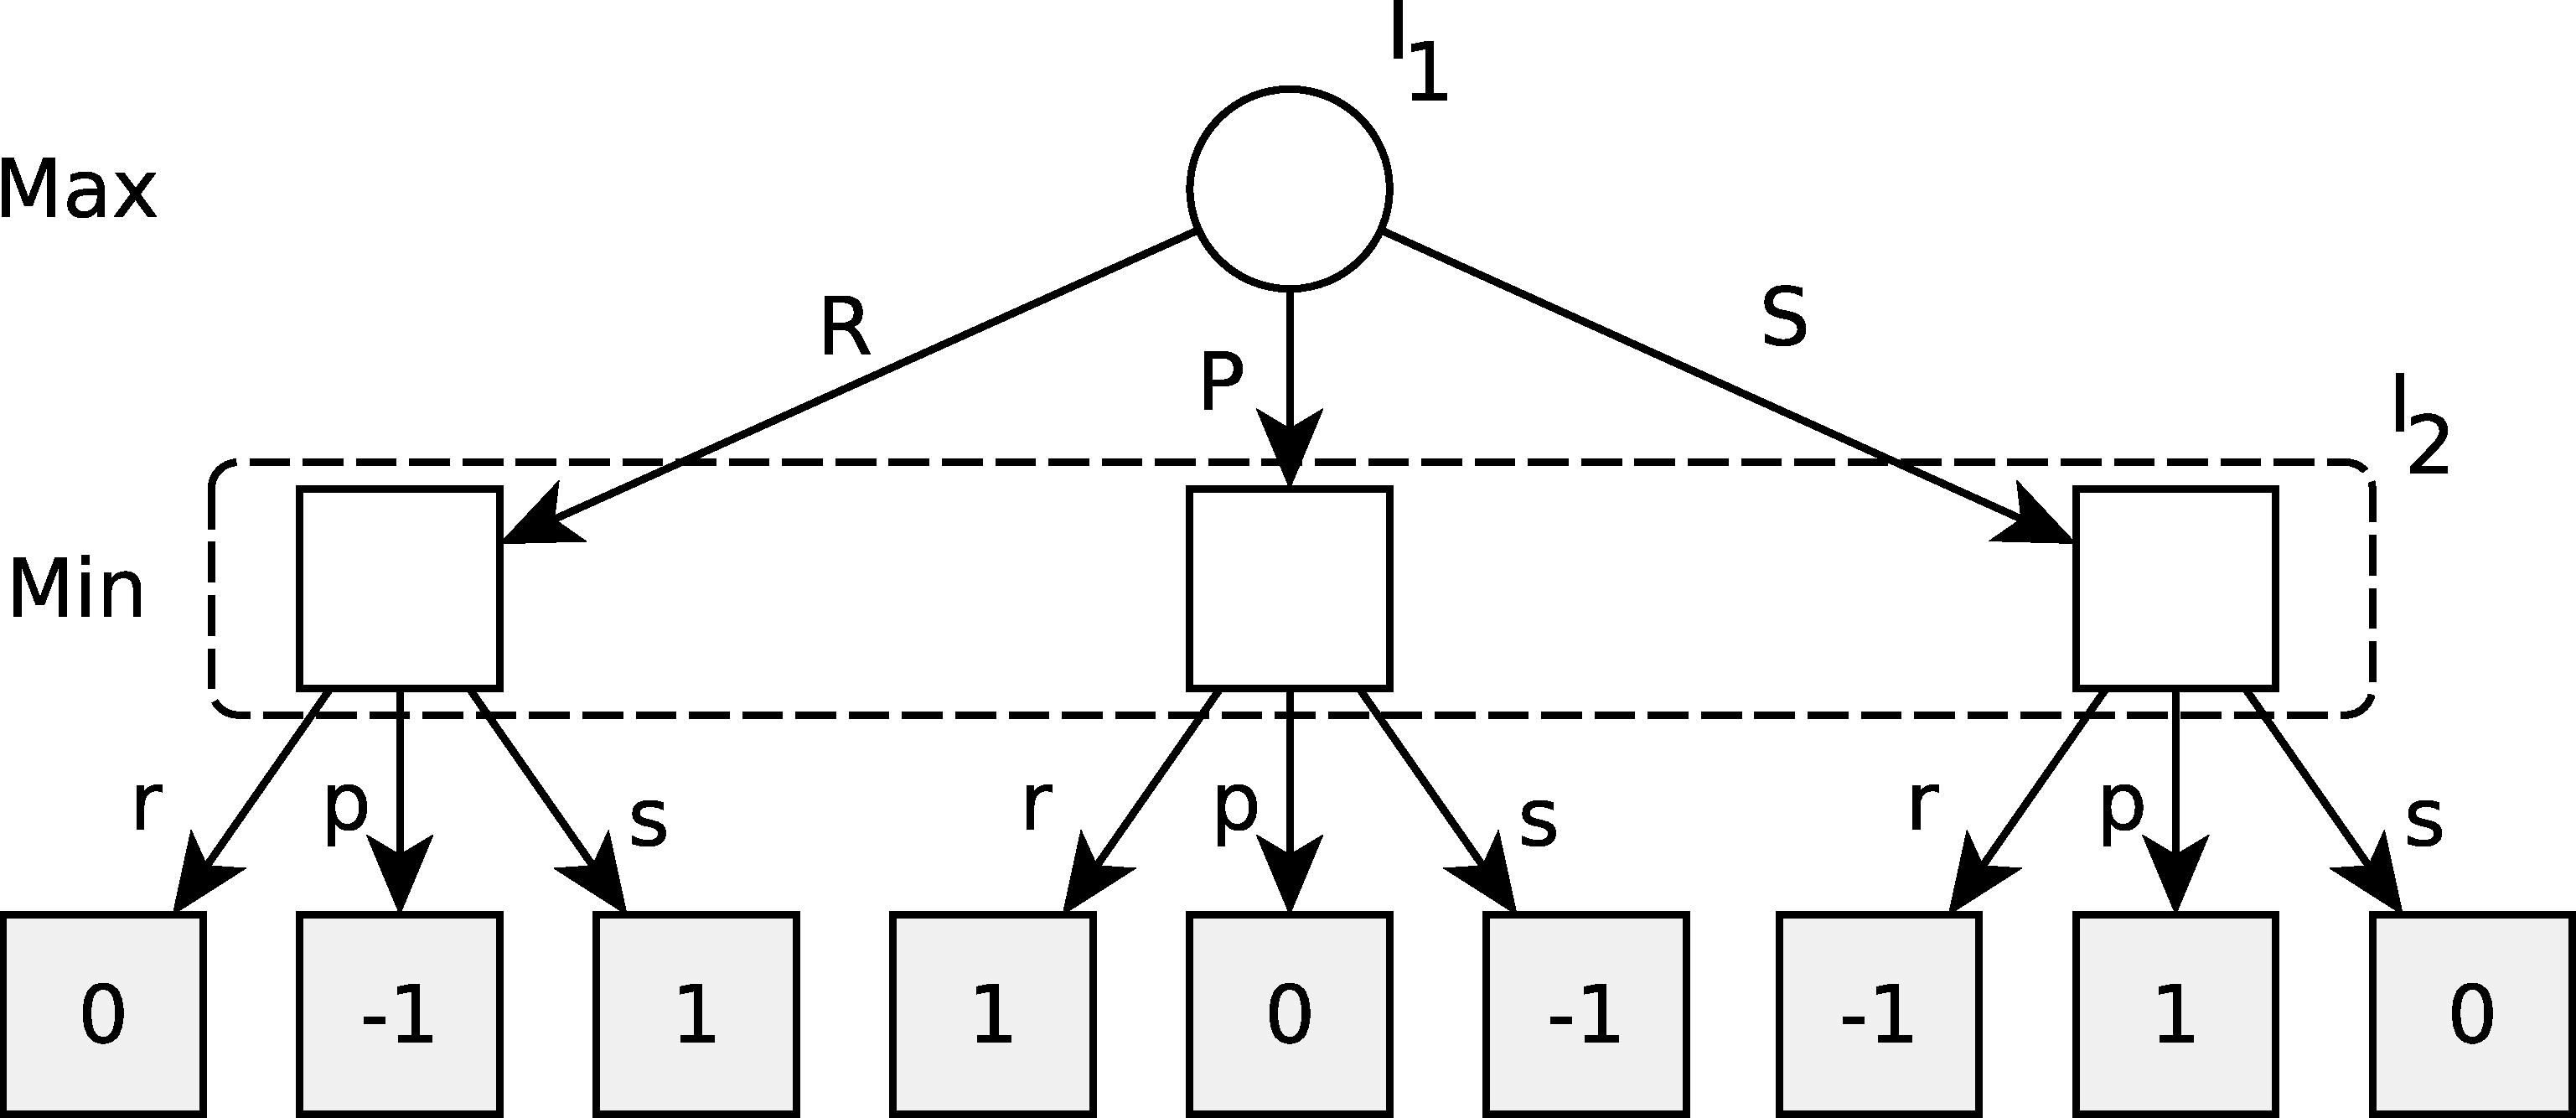
\includegraphics[width=0.6\textwidth]{figures/rps-new} \\
\end{tabular}
\end{center}
\caption{The matrix game of Rock, Paper, Scissors (left) and its equivalent extensive-form game representation (right). The extensive
game has four states, two information sets ($I_1$ and $I_2$),
and nine terminal histories: $\{ Rr, Rp, Rs, Pr, Pp, Ps, Sr, Sp, Ss \}$. \label{fig:rps-equiv}}
\end{figure}




\section{Related Work} \label{sec:relwork}

There has been a number of algorithms designed for simultaneous move games that can be classified into three categories: 
(1) iterative learning algorithms, 
(2) exact backard induction algorithms, 
(3) approximative sampling algorithms.
The first type computes strategies through iterated self-play.
The second type computes a Nash equilibrium strategy of the game. 
The third type computes strategies by approximating utilities using sampling. 

\subsection{Iterative Learning Algorithms}

% mlanctot: I put this first because I thought historically it kind of made more sense.
%           Also, then it kind of leads into the ones that we will look at. 

% http://students.cs.byu.edu/~cs670ta/Fall2009/MinimaxQLearning.pdf
% http://www.ualberta.ca/~szepesva/papers/ml96.ps.pdf
% http://www.cogsci.rpi.edu/~rsun/si-mal/article3.pdf
% http://www.cs.duke.edu/~parr/uai2002.ps.gz

A significant amount of interest in simultaneous move games was generated by initial work 
on multiagent reinforcement learning. In multiagent reinforcement learning, each agent acts simultaneously and 
the joint action determines how the state changes. Littman introduced Markov games to model these interactions 
as well as a variant of Q-learning called Minimax-Q to compute strategies~\cite{Littman94markovgames,Littman01Value}.
Minimax-Q modifies the learning rule so that the value of the next state (the subgame) is obtained by solving
a linear program using the estimated values of that subgame's root.
As is common in these settings, the goal of each agent is to maximize their expected utility. 
In two-player zero-sum Markov games, an optimal policy corresponds to a Nash equilibrium strategy, which assures the agent 
the highest worst-case expected payoff. Initial results provided conditions under which approximate dynamic 
programming could be used to guarantee convergence to the optimal value function and 
policies~\cite{Littman96ageneralized}. Later, in \cite{Lagoudakis02}, Lagoudakis \& Parr provided stronger bounds 
and convergence guarantees for least squares temporal different learning using linear function approximation. 

At around this same time period, gradient ascent methods were introduced for playing 
repeated games~\cite{Singh20Nash,Bowling01WoLF}. These algorithms update strategies in a direction of the strategy space 
that increases expected payoff with respect to the opponent's strategy. These were then generalized and combined, and 
shown to minimize regret over time~\cite{Zinkevich03Online,Bowling05Convergence}, leading to strong convergence 
guarantees in multiagent learning. More no-regret algorithms followed and were applied to an imperfect information 
games in sequence-form (One-Card Poker)~\cite{Gordon06No}. Soon later, counterfactual regret (CFR) minimization was 
introduced for large imperfect information games~\cite{CFR}. CFR has gained much attention due to its success in 
computing Poker AI strategies, and in this paper we analyze the effectiveness of a specific form of Monte Carlo CFR 
for the first time in simultaneous move games. 

As we focus on zero-sum simultaneous move games in this paper, the work on multiagent learning in general-sum and 
cooperative games has been omitted. For surveys of the relevant previous work in multiagent 
reinforcement learning and game theory (including the zero-sum case), 
see~\cite{Nowe12MARLchapter,Busoniu08Comprehensive,Bloembergen15Evolutionary}.

\subsection{Exact Backward Induction Algorithms}

The techniques in this section are based on the backward induction algorithm (cf. \cite{Shoham09}), 
a form of dynamic programming~\cite{Bellman57} often presented for purely sequential games. 
A slightly modified variant of the algorithm can also be applied to simultaneous move 
games (e.g., see \cite{Ross71Goofspiel,buro2003,Rhoads12Computer}). 
%\bbosansky{We do need some better reference here.}) 
% mlanctot: added the Ross 1971 paper; as far as I know it's the earliest one. Would be nice to have a text book cover this.
The algorithm searches through the game tree in the depth-first manner and after computing the values of all the succeeding subgames, it solves the normal-form game corresponding to this state (i.e., computes a NE of the matrix game in the current state of the game), and propagates the calculated game value to the predecessor. The result of the backward-induction algorithm is a refinement of NE called \emph{subgame-perfect Nash equilibrium}. 

There are two notable algorithms that improve the standard backward induction in simultaneous move games. 
First is an algorithm by Saffidine et al.~\cite{Saffidine12SMAB} termed simultaneous move alpha-beta algorithm (SMAB). 
The main idea of the algorithm is to reduce the number of the recursive calls of the backward-induction algorithm by removing dominated actions in every stage game. The algorithm keeps bounds on the utility value for each successor in a game state. 
The lower and upper bounds represent the threshold values, for which neither of the actions of the player is dominated by any other action in the current matrix game. These bounds are calculated by linear programs in the state given existing exact values (or appropriate bounds) of the utility values of all the other successors of the state. If they form an empty interval (the lower bound is higher than the upper bound), pruning takes place and the dominated action is no longer considered in this state afterward. 
SMAB outperforms classical backward induction, however, the computational speed-up is only marginal. 

% mlanctot: This seems overly negative toward SMAB and I don't think we need to justify ourselves at this point in the paper. 
%           How about this.. in the evaluation section (next to the more impressive DOAB result) let's put something like:
%           Note: this saving is several orders of magnitude more than reported by SMAB~\cite{Saffidine12SMAB}. 
%SMAB outperforms classical backward induction, however, the computational speed-up is limited. 
%The reason is that computing dominated actions is a costly operation that does not prune many actions; hence, much of the game tree is still fully evaluated. The authors propose further enhancements in their work~\cite{Saffidine12SMAB}, however, these improvements are domain-specific heuristics and do not significantly change the overall performance of the algorithm. Since other exact algorithms achieve computation speed-up in several orders of magnitude compared to backward induction (as we show in Section~\ref{sec:eval}), we do not explicitly use SMAB in our experiments.
% bbosansky: Ok, I agree.

The second exact algorithm that is significantly faster compared to the classical backward induction was introduced in~\cite{Bosansky13Using}.
This algorithm is described in detail in Subsection~\ref{sec:doab}. The main idea is to integrate two key components: (1) instead of evaluating all successors in each state of the game and solving a normal-form game, the algorithm exploits the iterative framework known in game theory as double-oracle algorithm~\cite{McMahan03Planning}; (2) the algorithm computes bounds on the utility values of the successors by serializing the subgames and running classical alpha-beta algorithm. 

Finally, since simultaneous move games can be seen as standard extensive-form games with imperfect information, one can use techniques 
designed for large imperfect information games. 
An algorithm that is also built on double-oracle is the Range-of-Skill algorithm~\cite{Zinkevich07New}.  
However, the number of iterations required by this algorithm in the worst case can be large~\cite{Hansen08On}. 
There are also state-of-the-art algorithms for solving generic extensive-form games with imperfect information, based on sequence-form 
optimization problems~\cite{koller1996,Sandholm10The,bosansky2013-aamas}. 
However, these algorithms do not exploit the specific structure of simultaneous move games and could require memory that is linear 
in the size of the game tree. In practice, this prohibits scaling to larger games (see, \eg \cite{Saffidine12SMAB}) and causes weak performance
compared to tailored algorithms.

%\mlanctot{We should mention the Range-of-Skill algorithm \cite{Zinkevich07New} somewhere in this subsection. It was shown that there are very bad worst cases even for simple games \cite{Hansen08On}.. do we know if such bad cases are less likely to occur in simultaneous move games? It'd be nice if we could say anything at all on this.}\bbosansky{Not exactly sure how to approach this ... I have never really understood the benefits of ROS well.}

\subsection{Approximative Sampling Algorithms} \label{sec:related:sampling}

Monte Carlo Tree Search (MCTS) is a simulation-based state space search technique often used in extensive-form games \cite{Coulom06,UCT}. 
Having first seen practical success in computer Go \cite{Gelly2011,Gelly12}, MCTS has since been applied successfully to simultaneous move games and imperfect information games as well~\cite{Ciancarini10Kriegspiel}. 
Most of the successful applications use classical exploration/exploitation formula Upper Confidence Bounds (UCB)~\cite{UCB} as a selection strategy. These variants of MCTS are also known as UCT (UCB applied to trees). The first application of MCTS to simultaneous move games was in general game playing (GGP) \cite{GGP} programs: {\sc Cadiaplayer} \cite{Cadiaplayer,Finnsson12} uses UCB selection strategy for each player in a single game tree. The success of MCTS algorithm was demonstrated by success of {\sc Cadiaplayer} which was the top-ranked player of the GGP competition between 2007 and 2009, and also in 2012.

Despite this success, Shafiei et al. in \cite{Shafiei09} provide a counter-example showing that this straightforward application of UCT does not
converge to NE even in the simplest simultaneous move games and that a player playing a NE can exploit this strategy. Another variant of UCT, which has been applied to  Tron~\cite{Samothrakis10Tron}, builds the tree as if the players were moving sequentially giving one of the players an informational advantage. This approach also cannot converge to NE in general. For this reason, other variants of MCTS were considered for simultaneous move games. Teytaud and Flory describe a search algorithm for games with short-term imperfect information~\cite{Teytaud11Upper}, which are a generalization of simultaneous move games. Their algorithm uses a different selection strategy, called Exp3~\cite{Auer2003Exp3},
and was shown to work well in the Internet card game Urban Rivals. We provide details of these two main existing selection functions in Subsections~\ref{sec:duct} and~\ref{sec:exp3}.
A more thorough experimental investigation of different selection policies including UCB, UCB1-Tuned, UCB1-greedy, Exp3, and more is reported in the game of Tron \cite{Perick12Comparison}. The work by Lanctot et al.~\cite{Lanctot13Goofspiel} compares some of these variants and proposes Online Outcome Sampling, a search version of Monte Carlo CFR~\cite{Lanctot09Sampling}, which computes an approximate equilibrium strategy with high probability. We describe this algorithm in Subsection~\ref{sec:oos}.
Finally, Lisy et al.~\cite{lisy2013-nips} present variants of MCTS that provably converge to Nash equilibria in simultaneous move games, in general, using any regret-minimizing algorithm at each stage, showing observed worst-case behavior in several cases. 

There have been two recent studies that examine the head-to-head performance of these variants in practice. 
The first builds on previous work in Tron~\cite{Lanctot13Tron} by varying the shape of the initial board, 
comparing previous serialized variants of simultaneous move MCTS. The authors found that UCB1-Tuned worked 
particularly well in Tron when using knowledge-based playout policies. The success of UCB1-Tuned differed in 
a similar study of the same variants across nine domains~\cite{Tak14smmcts} without domain knowledge. In this 
work, the chosen games were ones inspired by previous work in general game playing and did not include chance elements. 
Results indicate that parameter-tuning landscapes do not seem as smooth as in the purely sequential case. 

% mlanctot: said enough about this paper already...
%Generally, head-to-head performance of UCB variants perform well, despite their theoretical shortcomings, with Oshi Zumo and 
%Goofspiel being notable exceptions where MCTS using a regret matching selection policy performs particularly well.

\subsubsection{Simulation-based Search in Real-time Games}

%\mlanctot{Brief overview of relevant work in RTS/video games}

Real-time games are not turn-based and represent a realistic physical situations where agents can move freely in space. 
The state of the game is a continuous function of time and the effect of some actions may only be realized some time 
after the decision is made. These games are often appropriately modeled as a simultaneous move game with very short 
delays (40 milliseconds) between frames. 

MCTS has enjoyed some success in these types of games, in the single-agent 
setting~\cite{Pepels14Monte,Perez14PTSP} and multiagent setting~\cite{Balla09UCT}, much of this work inspired by video 
games~\cite{Cowling13Video,BellemareNVB13,Ontanon13RTSSurvey}. Few of these works have considered MCTS
in the simultaneous move game directly. 
In one of the first papers on real-time strategy games, the authors used randomized serialization 
of the game~\cite{kovarsky2005heuristic}, or strategy simulation
from scripts was used to build a single matrix of values from which an equilibrium strategy was 
computed using linear programming~\cite{Sailor07adversarial}.  
This search can be extended to multiple nodes where internal nodes would correspond to scripts being interrupted to replan, similarly to \cite{lisy2009gbgts}.
MCTS-style multistage replanning was also applied to a real-time battle scenario which was also accurately
represented as a discrete simultaneous move game~\cite{Beard12Using}. Results of this work show and that multistage
forward replanning can improve upon single-stage forward planning, and can produce approximate Nash equilibrium strategies
when mixed strategies are computed at each stage during search.
Around the same time, a serialized (sequential) version of alpha-beta was proposed for simultaneous move games 
and run on combat scenarios~\cite{Churchill2012Fast}; this algorithm is described in greater detail in
Section~\ref{sec:algs:biab} as it forms the basis of the follow-up enhanced by
double-oracle, presented in Section~\ref{sec:algs:doab}.

In this paper, we focus on the analysis of different algorithms for two-player simultaneous move games. Therefore, 
problems arising from discrete modeling of continuous time and space remain outside the scope of this paper.

%The benefit of serializing the game is that bounds
%on the correct minimax value can be obtained for the underlying simultaneous move game. These bounds can be used to cut out
%parts of the game tree in backward induction algorithms, and is explained in detail in Section~\ref{sec:algs:biab}.







\section{Offline Strategy Computation} \label{sec:offline}


This section focuses on algorithms that compute strategies for simultaneous move games. 
The baseline algorithm for solving simultaneous-move games is backward induction~(Section~\ref{sec:algs:bi}).
Therefore, we start our description of the algorithms focusing on algorithms based on the backward induction, then we introduce algorithms based on no-regret learning and Monte Carlo sampling.
After formally describing the backward induction we present a modification that exploits quick calculation of upper and lower bounds in a simultaneous-move game~(Section~\ref{sec:algs:biab}).
Then, we further improve the algorithm by speeding up the calculation of NE in stage games, exploiting the iterative framework known as the double-oracle algorithm~(Seciton~\ref{sec:algs:doab}).
In Section~\ref{sec:algs:cfros} we present counterfactual regret minimization and its sampling variant outcome sampling. 
Finally, we describe Monte Carlo tree search for simultaneous move games in Section~\ref{sec:algs:smmcts}. 
%\bbosansky{CFR/MCTS introduction}

\subsection{Backward Induction}\label{sec:algs:bi}
Standard backward induction algorithm is based on the depth-first search that in each state of the game evaluates all successors, creates matrix game for the current state, solves the matrix game, and propagates back the value of the matrix game. The pseudocode of the algorithm is depicted in Algorithm~\ref{alg:backwardinduction}. When there is a chance node succeeding the current state $s$, the algorithm directly evaluates all successors of this chance node calculating an expected utility: the value of each subgame rooted in node $s'$ calculated by recursive call is weighted by the probability of the stochastic transition $\Delta_{\cT(s,r,c)}$~(line~\ref{alg:bi:recursive}).

\begin{algorithm2e}[t]
\small
\SetKwInOut{Input}{input}\SetKwInOut{Output}{output}
\Input{$s$ -- current matrix game; $i$ -- searching player}
\If{$s \in \cZ$} {\Return $u_i(s)$} \label{alg:bi:stop1}
\For{$r \in \cA_1(s)$}{
	\For{$c \in \cA_2(s)$} {
	$A_{rc} \leftarrow \sum_{s' \in S \;:\; \Delta_{\cT(s,r,c)}(s') > 0} \Delta_{\cT(s,r,c)}(s')\cdot \textrm{BI}(s',i)$ \label{alg:bi:recursive}\;	
	}
}
$v_s \leftarrow$ solve matrix game $A$\;
\Return $v_s$ \label{alg:bi:stop2}
\caption{Backward Induction.}\label{alg:backwardinduction}
\end{algorithm2e}

Once the algorithm evaluates the value of each possible subgame following the current state $s$, then the matrix game $A$ is complete and the algorithm solves the matrix game $A$ using standard linear program (LP) for solving normal-form games:
\begin{eqnarray}
\max & v_s & \\
\textrm{s.t.} & \sum_{a_i \in \cA_{i}}A_{a_i,a_{-i}} \cdot \delta^{s}_i(a_i) \geq v_s & \forall a_{-i} \in \cA_{-i}\\
& \sum_{a_{i} \in \cA_{i}} \delta^{s}_{i}(a_{i}) = 1 \\
& \delta^{s}_{i}(a_{i}) \geq 0 & \forall a_{i} \in \cA_{i} 
\end{eqnarray}
Using the linear programming, the algorithm computes the value of the matrix game, which is propagated to the predecessor~(line~\ref{alg:bi:stop2}). 
If the algorithm evaluates a terminal state, it directly returns the utility value of the state~(line~\ref{alg:bi:stop1}).

Solving the linear programs is the main computational bottleneck of the backward induction algorithm. Therefore, in the following algorithms, we try to avoid this step of the computation even for the price of multiple traversal of the game tree.

\subsection{Backward Induction with Serialized Alpha-Beta Bounds}\label{sec:algs:biab}
Backward induction algorithm can be easily enhanced by using bounds on the value of sub-games. 
These bounds can be calculated very quickly by using a transformation of a simultaneous-move game into a perfect information extensive-form game.
Consider a matrix game representing a simultaneous choice of both players.
This matrix can be serialized by discarding the notion of information sets; hence, letting one player to play first following by the play of the second player. 
The crucial difference between a serialized and a simultaneous-move matrix game is that the second player to move has an advantage of knowing what action has been played in a serialized game.
Therefore, the value of a serialized game where player $i$ is second to move is an upper bound on the value of the matrix game. 

\begin{figure}
\includegraphics[width=0.45\textwidth]{figures/serialization1-1.png}
\includegraphics[width=0.45\textwidth]{figures/serialization1-2.png}
\caption{Different serialization of a simultaneous move game.}\label{fig:serialization}
\end{figure}

An example of this serialization is depicted in Figure~\ref{fig:serialization} with the utility value in the leaves depicted only for the first player. 
If this player moves first (the left subfigure), then the value of this serialized game is the lower bound of the value of the game; if this player moves second (the right subfigure), then the value of this serialized game is the upper bound of the value of the game.\vlisy{Write (gray) values into the inner nodes.}
Since the serialized games are zero-sum perfect-information games in the extensive form, they can be solved very quickly by using classical AI algorithm such as alpha-beta or negascout.
If the values of both serialized games are equal, then this is equal also to the value of the game. This situation occurs in our example in Figure~\ref{fig:serialization}, where both serialized games have value equal to $3$.

Obtaining these bounds can speed-up the backward induction algorithm. 
Algorithm~\ref{alg:backwardinduction-ab} depicts the pseudocode.
When the backward induction starts evaluating successors of the current state, the algorithm calculates upper and lower bounds using alpha-beta algorithm on serialized variants of the subgame rooted in the successor $s'$ (lines~\ref{alg:biab:ab1}-\ref{alg:biab:ab2}). The serialized game is solved using standard alpha-beta algorithm, where the second player \vlisy{Unfinished sentence?}
If the bounds are equal, the algorithm stores the value (line~\ref{alg:biab:saving}) instead of performing a recursive call~(line~\ref{alg:biab:recursive}). \jcermak{The only part mentioning strategy retrieval, should it be moved to online alg. description?} When such a cut-off occurs, one needs to extract the strategy from alpha-beta. Since the alpha-beta operates on a serialized version of the game, the actions played by the player with the additional information caused by observing the choice of his opponent cannot be used. This player is not forced to play according to the Nash equilibrium of the original non-serialized game, because the serialized game permits him to choose different action for every choice of the first player. And so one needs to extract the strategy for player $i$ from alpha-beta where $i$ plays first. The same goes for the strategy of $-i$.

\begin{algorithm2e}[t]
\small
\SetKwInOut{Input}{input}\SetKwInOut{Output}{output}
\Input{$s$ -- current matrix game; $i$ -- searching player}
\If{$s \in \cZ$} {\Return $u_i(s)$} \label{alg:biab:stop1}
\For{$r \in \cA_1(s)$}{
	\For{$c \in \cA_2(s)$} {
		$A_{rc} \leftarrow 0$\;
		\For{$s' \in S \;:\; \Delta_{\cT(s,r,c)}(s') > 0$} {
		$v^i_{s'} \leftarrow \textrm{alpha-beta}(s',i)$\; \label{alg:biab:ab1}
		$v^{-i}_{s'} \leftarrow \textrm{alpha-beta}(s',-i)$\; \label{alg:biab:ab2}
		\If{$v^{-i}_{s'} < v^i_{s'}$} {
			$A_{rc} \leftarrow A_{rc} + \Delta_{\cT(s,r,c)}(s')\cdot \textrm{BI}\alpha\beta(s',i)$ \label{alg:biab:recursive}\;	
			}
		\Else{
			$A_{rc} \leftarrow A_{rc} + \Delta_{\cT(s,r,c)}(s')\cdot v^i_{s'}$ \label{alg:biab:saving}
			}
		}
	}
}
$v_s \leftarrow$ solve matrix game $A$\;
\Return $v_s$ \label{alg:biab:stop2}
\caption{Backward Induction with Serialized Bounds}\label{alg:backwardinduction-ab}
\end{algorithm2e}

\subsection{Backward Induction with Double Oracle and Serialized Bounds}\label{sec:algs:doab}
Solving a matrix game can be further improved by using iterative double-oracle algorithm~\cite{McMahan03Planning}. 
First of all, we describe the main principles of the double-oracle algorithm in matrix games, following by describing the application of the algorithm in simultaneous-move game~\cite{Bosansky13Using}.

\subsubsection{Double-oracle Algorithm for Matrix Games}\label{sec:doab}
\begin{figure}
\centering
\includegraphics[width=0.8\textwidth]{figures/DO-scheme}
\caption{Schematic of the double-oracle algorithm for a normal-form game.}\label{fig:do-scheme}
\end{figure}

The main goal of the double-oracle algorithm is to find a solution of a matrix game without a need to construct the complete linear program that solves this game. 
The main idea is to create a restricted game by restricting the players to choose only from a limited set of actions.
Then the algorithm iteratively expands the restricted game by allowing the players to choose from new actions.
The new actions are allowed in iterations; each iteration a best response to an optimal strategy of the opponent in the current restricted game is allowed to be played in the restricted game.

Figure~\ref{fig:do-scheme} shows a visualization of the main structure of the algorithm, where the following three steps repeat until convergence:
\begin{enumerate}
\item create a restricted matrix game by limiting the set of actions that each player is allowed to play
\item compute a pair of Nash equilibrium strategies in this restricted game using linear programming
\item for each player, compute a pure best response strategy against the equilibrium strategy of the opponent; pure best response can be \emph{any} action from the original unrestricted game
\end{enumerate}
The best response strategies computed in step 3 are added to the restricted game, the game matrix is expanded by adding new rows and columns, and the algorithm follows with the next iteration. The algorithm terminates if neither of the players can improve the outcome of the game by adding a new strategy to the restricted game; hence, players play best response strategies to the strategy of the opponent. The algorithm maintains the values of expected utilities of the best-response strategies throughout the iterations of the algorithm. These values provide bounds on the value of the original game $v^*$

\subsubsection{Integrating Double-Oracle with Backward Induction}
\begin{algorithm2e}[t]
\small
\SetKwInOut{Input}{input}\SetKwInOut{Output}{output}
\Input{$s$ -- current matrix game; $i$ -- searching player; $\alpha_s,\beta_s$ -- bounds for the game value rooted in state $s$}
\If{$s \in \cZ$} {\Return $u_i(s)$} \label{alg:doab:stop1}
\If{$v_s^{-i} = v_s^i$} {
	\Return $v_s^{i}$
}
initialize $\cA'_i$, $\cA'_{-i}$ with arbitrary actions from $\cA_i, \cA_{-i}$\; \label{alg:doab:init}
\Repeat{$\alpha_s = \beta_s$}{
	\For{$r \in \cA'_i$, $c \in \cA'_{-i}$}{\label{alg:doab:restr1}
		\If{$A'_{rc}$ is not initialized}{
			 $A'_{rc} \leftarrow 0$\;
			\For{$s' \in S \;:\; \Delta_{\cT(s,r,c)}(s') > 0$} {
			$v^i_{s'} \leftarrow \textrm{alpha-beta}(s',i)$\; 
			$v^{-i}_{s'} \leftarrow \textrm{alpha-beta}(s',-i)$\; 
			\If{$v^{-i}_{s'} < v^i_{s'}$} {
				$A'_{rc} \leftarrow A'_{rc} + \Delta_{\cT(s,r,c)}(s')\cdot \textrm{double-oracle}(s',i,v^{-i}_{s'},v^i_{s'})$ \label{alg:doab:recursive}\;	
				}
			\Else{
				$A'_{rc} \leftarrow A'_{rc} + \Delta_{\cT(s,r,c)}(s')\cdot v^i_{s'}$ \label{alg:doab:saving}
				}
			}
		}	
	}
	$\left\langle v_s, \delta' \right\rangle \leftarrow $ solve matrix game $A'$\; \label{alg:doab:NE}
	$\left\langle v^{BR}_i, a^{BR}_{i} \right\rangle \leftarrow $ best-response$(i, \delta'_{-i}, \alpha_s)$\;\label{alg:doab:br1}
	$\left\langle v^{BR}_{-i}, a^{BR}_{-i} \right\rangle \leftarrow $ best-response$(-i, \delta'_{i}, \beta_s)$\; \label{alg:doab:br2}
	$\alpha_s \leftarrow \max(\alpha_s, v^{BR}_i)$,
	$\beta_s \leftarrow \min(\beta_s, v^{BR}_{-i})$\; \label{alg:doab:bounds}
	$\cA'_i \leftarrow \cA'_i \cup \lbrace a^{BR}_i \rbrace$,
	$\cA'_{-i} \leftarrow \cA'_{-i} \cup \lbrace a^{BR}_{-i} \rbrace$ \label{alg:doab:expand}
}
\Return $v_s$ \label{alg:doab:stop2}
\caption{Double Oracle with Serialized Bounds}\label{alg:doab}
\end{algorithm2e}

Double-oracle algorithm for matrix games can be directly incorporated into the backward induction -- instead of immediately evaluating each of the successors of the current game state and solving the linear program, the algorithm can exploit the double-oracle algorithm. Pseudocode in Algorithm~\ref{alg:doab} depicts this integration. In each state of the game, the algorithm initializes the restricted game with an arbitrary action (line~\ref{alg:doab:init}). Afterwards, the algorithm needs to evaluate each of the successors of the restricted game, for which the current value is not known (lines~\ref{alg:doab:restr1}-\ref{alg:doab:saving}). This evaluation is same as for backward induction with alpha-beta algorithm. 

Once all values for the restricted game $A'$ are known, the algorithm solves the restricted game (line~\ref{alg:doab:NE}) and keeps the optimal strategies $\delta'$ of the restricted game. Next, the algorithm calculates best responses for each of the player~(lines~\ref{alg:doab:br1},\ref{alg:doab:br2}), and updates the lower and upper bounds (line~\ref{alg:doab:bounds}). Finally, the algorithm expands the restricted game with best response actions (line~\ref{alg:doab:expand}) until the lower and upper bound are equal. In this case, neither of the best responses improves the current solution from the restricted game; hence, the algorithm has found an equilibrium of the complete unrestricted matrix game corresponding to state $s$.


\begin{algorithm2e}[t]
\small
\SetKwInOut{Input}{input}\SetKwInOut{Output}{output}
\Input{$s$ -- current matrix game; $i$ -- best-response player; $\lambda$ -- bound for the best-response value; $\delta'_{-i}$ -- strategy of the opponent }
$v^{BR}_i \leftarrow \lambda$ \;
$a_i^{BR} \leftarrow \textbf{null}$ \;
\For{$a_i \in \cA_i $\label{alg:br:start}} {%\setminus \cA'_i 
	$v_{a_i} \leftarrow 0$\;
	\For{$a_{-i} \in \cA'_{-i} \;:\; \delta'_{-i}(a_{-i}) > 0$} {\label{alg:br:opp}
		$\lambda_{a_i} \leftarrow \frac{v_i^{BR} - \sum_{a'_{-i} \in \cA'_{-i} \setminus \lbrace a_{-i} \rbrace} \delta'_{-i}(a'_{-i}) \cdot v^i_{\cT(s,a_i,a'_{-i})}}{\delta'_{-i}(a_{-i})}$\; \label{alg:br:bound}
		\If{	$\lambda_{a_i} > v^i_{\cT(s,a_i,a_{-i})}$}{
		continue from line~\ref{alg:br:start} with next $a_i$
		}
		\Else{
		\For{$s' \in S \;:\; \Delta_{\cT(s,a_i,a_{-i})}(s') > 0$} {
%			$v^i_{s'} \leftarrow \textrm{alpha-beta}(s',i)$\; \label{alg:br:ab1}
%			$v^{-i}_{s'} \leftarrow \textrm{alpha-beta}(s',-i)$\; \label{alg:br:ab2}
			\If{$v^{-i}_{s'} < v^i_{s'}$} {
				$v_{a_i,a_{-i}} \leftarrow v_{a_i,a_{-i}} + \Delta_{\cT(s,a_i,a_{-i})}(s')\cdot$ $\textrm{double-oracle}(s',i,v^{-i}_{s'},v^i_{s'})$\label{alg:br:recursive}\;	
				}
			\Else{
				$v_{a_i,a_{-i}} \leftarrow v_{a_i,a_{-i}} + \Delta_{\cT(s,a_i,a_{-i})}(s')\cdot v^i_{s'}$ \label{alg:br:saving}
				}
			}
			$v_{a_i} \leftarrow v_{a_i} + \delta'_{-i}(a_{-i})\cdot v_{a_i,a_{-i}}$\;		
		}
	}
	\If{$v_{a_i} > v_i^{BR}$}{\label{alg:br:max}
		$v_i^{BR} \leftarrow v_{a_i}$\;
		$a_i^{BR} \leftarrow a_i$\label{alg:br:save}
	} 
}
\Return $\langle v_i^{BR}, a_i^{BR} \rangle$ 
\caption{Best Response with Serialized Bounds}\label{alg:br}
\end{algorithm2e}

Next, we describe the algorithm for calculating the best responses. 
The pseudocode of the algorithm is depicted in Algorithm~\ref{alg:br}.
The goal of the algorithm is to find the best action from the original unrestricted game against current strategy of the opponent $\delta'$. 
Throughout the algorithm we use, as before, $v^i_{s'}$ to denote the upper bound of the value of the sub-game rooted in state $s'$ calculated using alpha-beta$(s',i)$. These values are calculated on demand, i.e., they are calculated once needed and cached until the game for state $s$ is not solved.
Moreover, once the algorithm calculates the exact value of a particular subgame, both upper and lower bounds are updated to be equal to actual value of the game. 

The algorithm iteratively tries all actions of player $i$ from the unrestricted game (line~\ref{alg:br:start}). 
Every action $a_i$ is evaluated against the actions of the opponent that are used in the optimal strategy from the restricted game (line~\ref{alg:br:opp}).
Before evaluating against an action of the opponent the algorithm determines, whether the current action of the searching player, $a_i$, can still be the best response action (line~\ref{alg:br:bound}). 
The value $\lambda_{a_i}$ represents the lowest possible expected utility this action must gain against the current action of the opponent $a_{-i}$. 
If this value is strictly higher than the upper bound of the successor (i.e., the value $v^i_{\cT(s,a_i,a_{-i})}$) than the algorithm knows that the action $a_i$ can never be the best response action, and the algorithm proceeds with the next action.
$\lambda_{a_i}$ is calculated by subtracting from the current best response value ($v_i^{BR}$) upper bound of the expected value against all other actions of the opponent ($v^i_{\cT(s,a_i,a'_{-i})}$). Recall, that these values are updated once the algorithm calculates exact values.

If the currently evaluated action $a_i$ can still be the best response, the value of the successor is determined (first by comparing the bounds). Once the expected outcome against all actions of the opponent is evaluated, the expected value of action $a_i$ is compared against the current best-response value (line~\ref{alg:br:max}) and saved, if the expected utility is higher~(line~\ref{alg:br:save}).

\subsection{Simultaneous-Move Monte Carlo Tree Search (SM-MCTS)} \label{sec:algs:smmcts}

Monte Carlo Tree Search (MCTS) is a simulation-based state space search algorithm often used
in game trees. The nodes in the tree represent game states. The main idea is to iteratively run
simulations to a terminal state, incrementally growing a tree rooted at the initial state of the game. In
its simplest form, the tree is initially empty and a single leaf is added each iteration. Each iteration
starts by visiting nodes in the tree, selecting which actions to take based on a selection function and
information maintained in the node. Consequently, the algorithm transitions to a successor state. When a
node is visited whose immediate children are not all in the tree, the node is expanded by adding a
new leaf to the tree. Then, \emph{a rollout policy} (e.g., random action selection) is applied from the new
leaf to a terminal state. The outcome of the simulation is then returned as a reward to the new leaf
and the information stored in the tree is updated.

\begin{algorithm2e}[t]
\small
\SetKwInOut{Input}{input}\SetKwInOut{Output}{output}
\Input{$s$ -- current state of the game}
\If{$s \in \cZ$} {
	\Return $u_1(s)$\;
}
\If{$s \in \cC$} {
        Sample $s' \sim \Delta_c(s)$\;
	\Return SM-MCTS($s'$)\;
}
\If{$s \in T$} {
	$(a_1, a_2) \leftarrow$ \emph{\underline{Select}}$(s)$\;\label{alg:smmcts:select}
	$s' \leftarrow \cT(s,a_1,a_2)$\;
	$v_{s'} \leftarrow $ SM-MCTS($s'$)\;\label{alg:smmcts:reccall}
	\emph{\underline{Update}}$(s,a_1,a_2,v_{s'})$\;\label{alg:smmcts:up}
	\Return $v_{s'}$\;
}
\Else{
	$T \leftarrow T \cup \lbrace s \rbrace$\;
	$v_{s} \leftarrow$ Rollout($s$)\;
	\Return $v_{s}$\;
}
\caption{Simultaneous Move Monte Carlo Tree Search}\label{alg:smmcts}
\end{algorithm2e}

We first present a generic template of MCTS algorithms for simultaneous move games (SM-MCTS) and then explain specific algorithms derived form this template.
Algorithm~\ref{alg:smmcts} describes a single iteration of the SM-MCTS. 
$T$ represents the MCTS tree, in which each state is represented by one node.
Every node $s$ maintains algorithm-specific statistics about the iterations that previously used this node.
The template can be instanciated by specific implementations of the updates of the statistics on line~\ref{alg:smmcts:up} and the selection based on these statistics on line \ref{alg:smmcts:select}.
In the terminal states, the algorithm returns the value of the state for the first player (line 2).
In the chance nodes, the algorithm selects one of the possible next stated based on the chance distribution (line 4).
If the current state has a node in the current MCTS tree $T$, the statistics in the node are used to select an action for each player (line~\ref{alg:smmcts:select}.
These actions are executed (line 8) and the algorithm is called recursively on the resulting state (line 9).
The result of this call is used to update the statistics maintained for state $s$ (line~\ref{alg:smmcts:up}).
If the current state is not stored in tree $T$, it is added to the tree (line 13) and its value is estimated usinf the rollout policy (line 14).

Different algorithms can be the bases for the selection functions (e.g., UCB~\cite{UCB}, Exp3~\cite{Auer2003Exp3}).
We now present the variants of SM-MCTS that were consistently the most successful in previous works, though more variants can be found in~\cite{Perick12Comparison,Lanctot13Tron,Tak14smmcts}.
Several examples are depicted in \cite{Tak14smmcts}. 

\subsubsection{Decoupled Upper-confidence Bound applied to Trees}\label{sec:duct}

The most common selection function for SM-MCTS is the Decoupled Upper-confidence Bound applied to Trees(DUCT).
For selection and updates, it executes the well-known UCT \cite{UCT} algorithm independently for each of the players in each nodes.
The statistics stored in search nodes are independently computed for each action of each player. For player $i\in \cN$ and action $a_i \in \cA_i(s)$ the reward sums $X_{a_i}$ and the number of times the action was used $n_{a_i}$ are maintained.
When a joint action needs to be selected by the \emph{\underline{Select}} function, an action that maximizes the UCB value over their reward estimates is selected for each player independently:
\begin{equation}
a_i = \argmax_{a_i \in \cA_i(s)}{ \left\{ \bar{X}_{a_i} + C_i \sqrt{\frac{\log n_s}{n_{a_i}}} \right\} },
  \mbox{ where } \bar{X}_{a_i} = \frac{X_{a_i}}{n_{a_i}} \mbox{ and } n_s=\sum_{b_i \in \cA_i(s)} n_{b_i}.
\end{equation}
\noindent The \emph{\underline{Update}} function increases the visit count and rewards for each player $i$ and its selected action $a_i$ using $X_{a_i} \leftarrow X_{a_i} + u_i$
and $n_{a_i} \leftarrow n_{a_i} + 1$.



Note that UCT does not define what happens which action is selected if multiple actions have identical value in the maximization. It is not relevant in sequential games, but it can have large impact in simultaneous move games. Consider the following matrix game
\begin{tiny}
$\left(\begin{array}{cc}
0 & 1\\
-1 & 0
\end{array}\right)$
\end{tiny}.
It has only one NE, such that both players play the first action. However, DUC selecting the first or the last action among the options with the same value will always get only the rewards 0 and the bias term will cause the players to round-robin over the diagonal indefinitely. This is clearly not optimal, as each player can than improve by playing first action with probability 1. However, if we choose the action to play randomly among the once with the same probability, DUCT will quickly converge to the optimal solution. Therefore, we use the randomized variant in our implementation.

After all the simulations are done, there are two options how to determine the resulting action to play.
The more standard option is to choose for each state the action $a_i$ that maximizes $n_{a_i}$ for each player $i$.
This is suitable mainly for games, in which using mixed strategy is not necessary.
Alternatively, the action to play in each state can be determined based on the mixed strategy obtained by normalizing the visit counts of each action 
\begin{equation}
\sigma_i(a_i) = \frac{n_{a_i}}{\sum_{b_i\in \cA_i(s)} n_{b_i}}.
\end{equation}
We call the former DUCT(max) and the latter DUCT(mix).
Using the first method will certainly not make the algorithm converge to a Nash equilibirum, because the game may require a mixed strategy.
The second has been shown not to converge to a Nash equilibrium as well; a counter-example in Rock, Paper, Scissors with biased payoffs is shown in \cite{Shafiei09}.

Even though DUCT is not guaranteed to converge to the optimal solution, it is often very successful in practice.
It has been used in and general game playing~\cite{Finnsson12}, in the Internet card game Urban Rivals~\cite{Teytaud11Upper},
and in the simultaneous move game Tron~\cite{Perick12Comparison}.
\mlanctot{Is there an earlier Tron paper where it was used?}
Note that DUCT is different than UCT run on a game that is transformed to perfect information by serialization of the simultaneous moves,
because in the latter case one player has the advantage of knowing what the other player chose at every stage.
\vlisy{Possibly mention convergence in games with pure strategies.}

\subsubsection{Exponential-weight algorithm for Exploration and Exploitation}\label{sec:exp3}

The second most common instantiation of SM-MCTS is to use the Exponential-weight algorithm for Exploration and Exploitation (Exp3) algorithm \cite{Auer2003Exp3} independently for each of the players.
In Exp3, each player maintains an estimate of the sum of rewards for each action, denoted $\hat{X}_{a_i}$. The joint action produced by \emph{\underline{Select}} is composed of an action independently selected for each player.
The probability of using action $a_i$ is proportional to the exponential of the reward estimates:
\begin{equation}\label{eq:exp3select}
\sigma_i(a_i) = \frac{(1-\gamma) \exp(\eta \hat{X}_{a_i})}{\sum_{b_i \in \cA_i(s)} \exp(\eta \hat{X}_{b_i})} + \frac{\gamma}{|\cA_i(s)|},
  \mbox{ where } \eta = \frac{\gamma}{|\cA_i(s)|}.
\end{equation}

This standard formulation of Exp3 is suitable for deriving its properties, but a straightforward implementation of this formula leads to problems with numerical stability. Both the numerator and denominator of the fraction can quickly become too large. For this reason, numerically more stable formulations has been suggested, e.g., in \cite{Lanctot13Goofspiel} and \cite{Cowling12ISMCTS}. We use the following quivalent formulation from \cite{Cowling12ISMCTS}:
\begin{equation}
\sigma^t_i(a_i) = \frac{(1-\gamma)}{\sum_{b_i \in A_i(s)}\exp(\eta(\hat{X}_{b_i}-\hat{X}_{a_i}))}
\end{equation}

The update after selecting actions $(a_1,a_2)$ and obtaining a simulation result $v_1$ normalizes the result to the unit interval for each player by
\begin{equation}
u_1 \leftarrow \frac{(v_1 - v_{min})}{v_{max} - v_{min}};\;\; u_2 \leftarrow (1-u_1)
\end{equation}
and adds to the corresponding reward sum estimates the reward divided by the probability that the action was played by the player using
\begin{equation}
\hat{X}_{a_i} \leftarrow \hat{X}_{a_i} + \frac{u_i}{\sigma_i(a_i)}.
\end{equation}
Dividing the value by the probability of selecting the corresponding action makes $\hat{X}_{a_i}$ estimate the sum of rewards over all
iterations, not only the once where $a_i$ was selected.

As the final strategy, after all iterations are executed, the algorithm computes the \emph{average strategy} of the Exp3 algorithm over all iterations for each player. After $n$ iterations in the particular node, it is
\begin{equation}
\bar{\sigma}^t_i(a_i) = \frac{1}{n}\sum_{t=1}^n \sigma^t_i(a_i).
\end{equation}
In our implementation, we maintain the cumulative sum and normalize it to obtain the average strategy after the iterations.

Previous work \cite{Teytaud11Upper} suggests first removing the samples caused by the exploration.
This modification proved to be useful also in our experiments and it has been shown not to reduce the performance substantially in the worst case \cite{kovarik}, \mlanctot{Add missing reference} so as the resulting final mixed strategy, we use
\begin{equation}
\bar{\sigma}_i(a_i) \leftarrow \max\left(0, \bar{\sigma}_i(a_i) - \frac{\gamma}{|\cA_i(s)|}\right),
\end{equation}
normalized to sum to one.

\subsubsection{Regret Matching} \label{sec:rm}

This variant applies regret matching \cite{Hart00} to the current estimated matrix game at each stage. The statistics stored by this algorithm in each node are the use count of each joint action ($n_{a_1a_2}$), the sum of rewards for each joint action ($X_{a_1a_2}$). Furthermore, the algorithm for each player $i$ maintains a cumulative regret $r^i_{a_i}$ for having played $\sigma_i^t$ instead of $a_i \in \cA_i(s)$ on iteration $t$, initially set to 0. The regret values $r^i_{a_i}$ are maintained separately by each player, as in DUCT. However, the updates uses a value that is a function of the joint action space. 

On iteration $t$, function \emph{\underline{Select}} first builds
each player's current strategies from the cumulative regrets. Define $x^+ = \max(x,0)$,
\begin{equation}
\label{eq:rm}
\sigma^t_i(a_i) = \frac{r^{i+}_{a_i}}{R^+_{sum}} \mbox{ if } R^+_{sum} > 0 
\mbox{ oth. } \frac{1}{|\cA_i(s)|}, \mbox{ where } R^+_{sum} = \sum_{b_i \in \cA_i(s)}{r^{i+}_{b_i}}.
\end{equation}
The main idea is to adjust the strategy by assigning higher weight proportionally to actions based on the regret of having not taken them over the long-term.
To ensure exploration, an $\gamma$-on-policy sampling procedure similar to Equation~\ref{eq:exp3select} is used
choosing action $a_i$ with probability $\gamma/|\cA(s)| + (1-\gamma) \sigma^t_i(a_i)$.

\emph{\underline{Update}} adds regret accumulated at the iteration to
the regret tables $r^i$. Suppose joint action $(a_1,a_2)$ is
sampled from the selection policy and utility $v_1$ is returned from the recursive call on line~\ref{alg:smmcts:reccall}.
Label $reward(b_1,b_2) = \frac{X_{b_1b_2}}{n_{b_1b_2}}$ if
$(b_1,b_2) \not= (a_1,a_2)$, or $v_1$ otherwise. The updates to the regret are:
\begin{eqnarray}
\forall b_1 \in \cA_1(s), ~~  r^1_{b_1} \leftarrow r^1_{b_1} + ( reward(b_1, a_2) - v_1 ),\\
\forall b_2 \in \cA_2(s), ~~  r^2_{b_2} \leftarrow r^2_{b_2} - ( reward(a_1, b_2) - v_1).
\end{eqnarray}
%\noindent and average strategy updates for each player, $\bar{\sigma}^i_s[a] \leftarrow \bar{\sigma}^i_s[a] + \sigma^t_i(s,a).$

After all simulations, the strategy to play in state $s$ is defined by the mean strategy used in the corresponding node as in case of Exp3.

\subsection{Counterfactual Regret Minimization and Outcome Sampling} \label{sec:algs:cfros}

Counterfactual Regret (CFR) is a notion of regret at the information set level for extensive-form games with imperfect information~\cite{CFR}.
The CFR algorithm iteratively learns strategies in self-play, producing approximate equilibrium strategues over time. 

Define a {\it history} as a sequence of actions taken by all players (including chance) that starts from the beginning of the game. 
A history $h'$ is a prefix of another history $h$, denoted $h' \sqsubset h$, if $h$ contains $h'$ (as a prefix sequence of actions).  
The {\it counterfactual value} of reaching information set $I$ is the expected payoff given that player $i$ played to reach $I$, the opponents played
$\sigma_{-i}$ and both players played $\sigma$ after $I$ was reached:
\begin{equation}
\label{eq:cfv}
v_i(I,\sigma) = \sum_{(h,z) \in Z_I} \pi^{\sigma}_{-i}(h) \pi^{\sigma}_{i}(h,z) u_i(z), 
\end{equation}
where $Z_I = \{ (h,z)~|~z \in Z, h \in I, h \sqsubset z \}$.
Suppose, at time $t$, player $i$ plays with strategy $\sigma^t_i$.
Define $\sigma^t_{I \rightarrow a}$ as identical to $\sigma^t$ except at $I$ action $a$ is taken with probability $1$.
The counterfactual regret of not taking $a \in A(I)$ at time $t$ is $r^t(I,a) = v_i(I,\sigma^t_{I \rightarrow a}) - v_i(I,\sigma^t)$.
The CFR algorithm maintains the cumulative regret $R^T(I,a) = \sum_{t=1}^T r^t(I,a)$, for every action at every information set.
Then, the distribution at each information set for the next iteration $\sigma^{T+1}(I)$ is obtained individually using
regret-matching~\cite{Hart00}. The distribution is proportional to the positive portion of the individual actions' regret:
\begin{equation*}
\label{eq:rm}
\sigma^{T+1}(I,a) = \left\{
\begin{array}{ll}
R^{T,+}(I,a) / R^{T,+}_{sum}(I) & \mbox{if } R^{T,+}_{sum}(I) > 0 \\ 
1 / |A(I)|                   & \mbox{otherwise,}
\end{array} \right.
\end{equation*}
where $x^+ = \max(0,x)$ for any term $x$, and $R^{T,+}_{sum}(I) = \sum_{a' \in A(I)} R^{T,+}(I,a')$. 
Furthermore, the algorithm maintains for each information set the average   strategy profile
\begin{equation}
%\bar{\sigma}^T(I,a) = \frac{1}{T}\sum_{t=1}^T \sigma^t(I,a).
\bar{\sigma}^T(I,a) = \frac{\sum_{t=1}^T \pi^{\sigma^t}_i(I) \sigma^t(I,a)}{\sum_{t=1} \pi^{\sigma^t}_i(I)}, 
\end{equation}
where $\pi^{\sigma^t}_i(I) = \sum_{h \in I}\pi^{\sigma^t}_i(h)$.
The combination of the counterfactual regret minimizers in individual information sets also minimizes the overall 
average regret \cite{CFR}, and hence the average profile is a  $2\epsilon$-equilibrium, with $\epsilon \rightarrow 0$
as $T \rightarrow \infty$.

Monte Carlo Counterfactual Regret Minimization (MCCFR) applies CFR to sampled portions of the games~\cite{Lanctot09Sampling}.
In the {\it outcome sampling} (OS) variant, a single terminal history $z\in Z$ is sampled in each iteration.
The algorithm updates the regret in the information sets visited along $z$ using the
{\it sampled counterfactual value},
\begin{equation}
\tilde{v}_i(I,\sigma) = \left\{
\begin{array}{ll}
\frac{1}{q(z)} \pi^{\sigma}_{-i}(z) \pi^{\sigma}_{i}(h,z) u_i(z) & \mbox{if } (h,z) \in Z_I\\
0  & \mbox{otherwise,}
\end{array} \right.
\label{eq:scv}
\end{equation}
where $q(z)$ is the probability of sampling $z$.
As long as every $z \in Z$ has non-zero probability of being sampled, $\tilde{v}_i(I,\sigma)$ is an unbiased estimate of $v(I,\sigma)$
due to the importance sampling correction ($1/q(z)$). For this reason, applying CFR updates using these sampled counterfactual regrets
$\tilde{r}^t(I,a) = \tilde{v}_i(I,\sigma^t_{I \rightarrow a}) - \tilde{v}_i(I,\sigma^t)$
on the sampled information sets values also eventually converges to the approximate equilibrium of the game with high probability.
The required number of iterations for convergence is much larger, but each iteration is much faster.

%Pseudocode of outcome sampling is presented in the next subsection.

% Will put pseudocode in the Online part..?
%\begin{algorithm2e}[t]
%\small
%\SetKwInOut{Input}{input}\SetKwInOut{Output}{output}
%\Input{game $g$}
%\Return 1
%\caption{Outcome Sampling MCCFR}\label{alg:os}
%\end{algorithm2e}

\subsubsection{Online Outcome Sampling} \label{sec:oos}

Online Outcome Sampling (OOS) is a version of outcome sampling MCCFR described in 
Section~\ref{sec:algs:cfros}. It resembles MCTS in that it builds its tree incrementally, however it 
is based on outcome sampling MCCFR rather than on UCB. The algorithm as applied to full imperfect information
games is found in~\cite{Lanctot14OOS}. Here, we describe a simplified version specifically designed for 
simultaneous move games. 

% Note, mlanctot: \ElsIf breaks compilation for me but \ElseIf works
%bb: Interestingly, \ElseIf does not work for me, but \ElsIf does ... maybe different versions of algorithm2e ?
\begin{algorithm2e}[t]
\small
\SetKwInOut{Input}{input}\SetKwInOut{Output}{output}
\Input{$h$ -- current state of the game; $i$ -- current player; $\pi_i$ -- reach probability for player $i$; $\pi_{-i}$ -- reach probability for opponent of $i$, $s$ -- sample reach probability}
  \lIf{$h \in Z$}{\Return $(s, u_i(z))$} \label{alg:terminal}
  \ElsIf{$h$ is a chance node}{
    Sample outcome $a$ with probability $\Pr(a)$ \;
    \Return OOS$(ha, i, \pi_i, \pi_{-i}, s \cdot \Pr(a))$\;
  }
  $I \gets $ information set of player $P(h)$ at $h$ \;
  Sample $a \sim \Phi(I, i, \epsilon)$ with prob. $\Pr(a)$ \; \label{alg:sample}
  \If{$I$ is not in memory}{
    Add $I$ to memory \;
    $\sigma(I) \leftarrow \mbox{Unif}(A(I))$ \;
    $(q(z), u_i(z)) \gets $ Playout$(ha, s \cdot \Pr(a))$ \;         \label{alg:playout}
  }
  \Else{
    $\sigma(I) \gets $ RegretMatching$(R_I)$ \;
    $\pi_{P(h)}' \gets \sigma(I,a)\pi_{P(h)}$ \;    \label{alg:newreaches1}
    $\pi_{-P(h)}' \gets \pi_{-P(h)}$ \;             \label{alg:newreaches2}
    $(q(z), u_i(z)) \gets$ OOS$(ha, i, \pi_i', \pi_{-i}', s \cdot \Pr(a))$ \;
  }
  \For{$a' \in A(I)$}{
    \If{$P(h) = i$}{
      Update $R_I[a']$ for each $a' \in A(I)$ using $\tilde{r}^t(I,a)$ according to Eq.~\ref{eq:scv}
    }
    \Else{
      Update $S_I[a'] \gets S_I[a'] + \frac{1}{s} \pi_{-i} \sigma(I,a')$ for each $a' \in A(I)$ \;  \label{alg:avgstrat}
    }
  }
  \Return $(q(z), u_i(z))$ \;   \label{alg:returnend}
  \vspace{0.1cm}
  \caption{Simultaneous Move Online Outcome Sampling. \label{alg:oos}}
\end{algorithm2e}



One iteration of the algorithm requires, as input, the current state of the game and a player role $i$. 
Each iteration the player role $i$ is alternated. As the algorithm is applied to the imperfect information 
representation of the simultaneous move game (described in Section~\ref{sec:smg}), we use histories $h$ 
and information sets $I$ rather than states. 

An information set tree is incrementally built, starting with the searching player's root information set.
An information set stores two tables: $R_I$ stores the cumulative regret $R^T(I,a)$ for each action, 
and average strategy table $S_I$ which stores the cumulative average strategy contribution for each action. 
An $\epsilon$-on-policy sampling distribution used to sample actions, defined as
\begin{equation*}
\label{eq:ossample}
\Phi(I,i,\epsilon) = \left\{
\begin{array}{ll}
\epsilon \cdot \mbox{Unif}(A(I)) + (1-\epsilon)\sigma_i(I) & \mbox{if } P(I) = i\\ 
\sigma_i(I)                                          & \mbox{otherwise,}
\end{array} \right.
\end{equation*}
and denote $\Phi(I,i,\epsilon,a)$ the probability of sampling $a \in A(I)$.







\section{Online Search} \label{sec:online}

In this section, we describe online adaptations of the algorithms above and their application 
to any-time search within a limited time. 

\subsection{Iterative Deepening Backward Induction Algorithms} \label{sec:idbi}

Minimax search~\cite{AIbook} has been used with much success in sequential perfect information games, 
leading to superhuman strength in computer chess game play, one of the key advances of artifical 
intelligence. 
Minimax search is an online application of backward induction run on approximated game. 
The game is approximated by searching to a fixed depth limit $d$, treating the states at depth $d$
as terminal states, evaluating their values using a heuristic evaluation function, $v(s)$. 
The main focus is to compute an optimal strategy for this heuristic approximation of the original game. 

Under limited time settings, a search algorithm is given a fixed time budget to compute a strategy. 
We use a classical approach of {\it interative deepening}~\cite{AIbook} that runs several depth-limited 
minimax searches, starting at a low depth and iteratively increasing the depth of each successive search. 
Note that the depth limit of $d$ means that the algorithm will evaluate $d$ pairs of simultaneous actions, each pair possibly preceded by action of nature if present.  
%In sequential perfect information games, several enhancements can be applied due to researching the same 
%nodes, most of which are not immediately applicable in simultaneous move games. However, whether new 
%enhancements can be defined for this class of games remains an open research question. 
In our implementation of iterative deepening we follow a natural observation that a solution computed in state $s$ by player $i$ to depth $d$ contains depth $d-1$ solutions to all possible next states $\cT(s,a_i,?)$, where $a_i$ is the action selected for player $i$.
This allows us to start the iterative deepening in any state $s' \in \cT(s,a_i,?)$ with depth $d$.
If the time limit does not allow full evaluation of the sub-game with the root in $s'$, the algorithm reuses the result from previous computation.
In case there is no strategy stored for the state $s'$ due to pruning, iterative deepening is started with $d = 1$.

\subsection{Online Search using Sampling Algorithms}

\bbosansky{The following subsection is quite wordy -- feel free to make it more compact and technical.}
Using sampling algorithms in an online settings is simpler compared to the algorithms based on the backward induction, since no significant changes are needed and the algorithms do not need an evaluation function.
The algorithms are stopped after given time limit and the move to play or the complete strategy is extracted as described for each sampling algorithm in Section~\ref{sec:offline}.
There are two concepts that need to be discussed. 
First of all, the algorithms can re-use all information and statistics gained in previous iterations; hence, after returning a move and advancing to a succeeding state of the game $s'$, the subtree rooted in $s'$ of the incrementally built tree is preserved and used in the next iterations. 
Note that reusing the previously gathered statistics in the sub-tree rooted in $s'$ has no potentially negative effect on any variant of the MCTS algorithms since the behavior of the algorithm is exactly the same when the iteration is started in this node, or if this node is reached from its predecessor. On the other hand, this does not hold generally for OOS, where the regret values are weighted by the reach probabilities depending on the strategy used in the preceding nodes.  However, this fact does not negatively affect the convergence of the algorithm. In the definition of sampled counterfactual value in equation~\ref{eq:scv}, the value of the leaf sampled in the current iteration is scaled up by one over the probability of reaching the leaf. This scaling also translates to regret values. After the root of the game is moved to a sub-tree and therefore the samples are shorter, it will generally have a larger sample probability and smaller weight in the regret updates. As a result, the earlier and less precise samples have larger weight in cumulative regrets than the later iterations. On the other hand, with larger sample probability, the regrets will be updated much more often, and eventually overweight the older samples.\vlisy{This is still a little unclear, but it might be the reason why OOS dost not work well online. I have implemented a modified version and I will run some experiments.}

Secondly, even though the sampling algorithms do not require to use domain-specific knowledge for online search, they often incorporate this type of knowledge to better guide the sampling and thus to evaluate more relevant parts of the state space~\cite{Gelly07Combining,Lorentz08Amazons,Winands10MCTS-LOA,Lorentz13Breakthrough,Lanctot14Implicit}. When directly comparing sampling-based algorithms with the backward-induction algorithms that are clearly dependent on the evaluation function, the outcome of such a comparison strictly depends on the quality of the evaluation function -- in case of a very large game, a backward induction algorithm with precise evaluation function will be significantly better (we will see such examples in the experimental evaluation). Therefore, we also use sampling algorithms combined with and an evaluation function. The integration is done via replacing the random play-out that leads to the end of the game by directly using the value of the evaluation function in the current state for MCTS or OOS algorithms. 
Again, such a modification does not generally affect theoretical properties of the algorithms -- the proofs of the convergence (e.g., \cite{lisy2013-nips}) assume that a whole game tree is eventually built and any statistics in the nodes collected before (either by random play-outs or evaluation functions) can eventually be over-weighted. In the short time, for MCTS algorithms, there is no reason to believe that a good evaluation function would give better estimate of the quality of a sub-tree as a random play-out. The only complication can, again, be the probabilities in OOS. The weight of the sample in equation~\ref{eq:scv} is lowered by the probability of reaching the sampled leaf from the updated information set. When using $\gamma$-on-policy sampling, this ``tail'' probability is mostly cancelled by the probability of reaching the sampled leaf form the root in the denominator. If the sample is terminated earlier, it does not have a substantial effect on the scale of the regret updates.


%\reviewchange{
%\section{Theoretical Guarantees and Limitations}
%
What to include in this section?

\begin{enumerate}
\item Time and space complexities of each algorithm
\item Mention any theoretical properties (i.e. reference to upper/lower bound lemmas for serialized games)
\item Examples of worst and best cases and what effect this can have on the algorithms
\item An overview of our NIPS paper convergence results for sample-based algorithms
\end{enumerate}

 \label{sec:theory}
%}

\section{Empirical Evaluation} \label{sec:eval}

%!TEX root = sm-journal.tex

We now turn to thorough experimental evaluation of the described algorithms.
We analyze both offline and online case on a collection of games inspired by games used for experimental evaluation in previous works, and randomly generated games.
After describing the rules of the games, we present the results for the offline strategy computation case and we follow with the online game playing.

\subsection{Experimental Settings}

%TODO: Remove 5s results, add paragraph + graph summary

We start with an experimental evaluation of a well-known example of Biased Rock, Paper, Scissors~\cite{Shafiei09} that often serves
as an example that MCTS with UCT selection function does not converge to a Nash equilibrium.
%\bbosansky{In the description of UCT we need to suggest that there are two things how to do it (deterministically, randomly) -- in the experiments only refer to this.} done
We reproduce this experiment and show the differences in performance of the sampling algorithms -- primarily the impact of randomization in UCT.
Then, we compare the offline performance of the algorithms on other domains.
For each domain, we first analyze the exact algorithms and measure the computation time taken to solve a particular instance of the game.
We compute mean out of at least $30$ runs for each game settings.
Afterwards, we analyze the convergence of the approximative algorithms.
At the specified time step the algorithm produces strategies $(\sigma_1,\sigma_2)$, and using best responses we compute
$\textrm{error}(\sigma_1,\sigma_2) = \max_{\sigma_1' \in \Sigma_1} \bE_{z \sim (\sigma_1',\sigma_2)}[u_1(z)]
                                   + \max_{\sigma_2' \in \Sigma_2} \bE_{z \sim (\sigma_1,\sigma_2')}[u_2(z)]$,
which is equal to $0$ at a Nash equilibrium.
In each offline convergence setting, the reported values are means out of at least $20$ runs of each sampling algorithm on a single instance of the game.
We compared at least $3$ different settings for the exploration parameter and present the result only for the best exploration parameter.
For OOS, Exp3, and RM the best values for the parameters were almost always $0.6$, $0.1$, and $0.1$.
\reviewchange{The only exception was Goofspiel with chance nodes, where both Exp3 and RM converge more quickly with parameter set to $0.3$.}
For UCT, however, the performance was quite different and we give the values for UCT for each domain.
% mlanctot: please check the definition of error
%\vlisy{is the 20 runs enough?}\bbosansky{this is the lowest number, some games (\eg, Goofspiel) had more samples (40)}

Finally, we turn to the comparison of the algorithms in the online setting and we present head-to-head tournament on each domain.
We used larger instances of games and calculated win-rate for each algorithm.
We use two different restrictions to computation time per move: 1 second and 5 seconds.\bbosansky{TODO @Vilo, remove the "5 seconds" when you finish with rewriting the online experiments.}
% mlanctot: we do not have to justify this choice
%The first one is more common in previous works focused on online comparison of the algorithms~\cite{XXX}\bbosansky{Reference missing -- ideally several works with different authors that use this settings.}, second one allows us to see the difference if the algorithms have more computation time.
As indicated before, the algorithms based on the backward induction need to use domain-specific evaluation function in the online settings.
This may give these algorithms an advantage if the evaluation function is very precise.
Therefore, for selected domains we also run sampling-based algorithms with an evaluation function to compare the algorithms in a more fair settings.
Reported results are mean of at least $1000$ matches for each pair of algorithms.
%Where necessary, we run additional experiments to obtain statistically significant results.

Each of the described algorithms was implemented in a generic framework for modeling and solving extensive-form games\footnote{Source code is available at \texttt{http://agents.felk.cvut.cz/topics/Computational\_\newline game\_theory}. We use IBM CPLEX 12.5 to solve the linear programs.}.
We are interested in the performance of the algorithms and their ability to find or approximate the optimal behavior.
Therefore, with the exception of the evaluation function used in selected online experiments, no algorithm is using any domain-specific knowledge.


\subsection{Domains}\label{sec:eval:domains}

In this subsection, we describe the six domains used in our experiments.
The games in our collection differ in characteristics, such as the number of available actions for each player (\ie the branching factor), maximal depth, and number of possible utility values.
Moreover, the games also differ in the \emph{randomization factor} -- \ie how often it is necessary to use mixed strategies and whether this randomization occurs at the beginning of the game, near the end of the game, or it is spread throughout the whole course of the game.

For each domain we also describe the evaluation function used in the online experiments.
Note that we are not seeking the best-performing algorithm for a particular game; hence, we have not aimed for the most accurate evaluation functions for each game.
We intentionally use evaluation functions of different quality that allow us to compare the differences between the algorithms from this perspective as well.

\paragraph{\textbf{Biased Rock, Paper, Scissors}}

BRPS is a payoff-skewed version of the one-shot game Rock, Paper, Scissors shown in
Figure~\ref{fig:brps}. This game was introduced in \cite{Shafiei09}, and it was shown that the visit count
distribution of UCT does converge to a fixed balanced situation, but not one that
corresponds to the optimal mixed strategy of $(\frac{1}{16},\frac{10}{16},\frac{5}{16})$.
% mlanctot: should be done for the whole section
%\vlisy{unify the use of UCT/DUCT}

%\item[Goofspiel] is a card game where each player gets 13 cards marked 1-13, and there is a face down
%point-card stack (also 1-13). Every turn, the {\it upcard} (top card of the point-card stack is turned face up,
%Each player chooses a {\it bid} card from their hand simultaneously.
%The player with the higher bid takes the upcard. The bid cards are then discarded and a new round starts.
%At the end of 13 rounds, the player with the highest number of points wins, a tie ends in a draw.

\begin{figure}[h!]
\begin{center}
\begin{tabular}{c|c|c|c|}
 \multicolumn{1}{c}{~} & \multicolumn{1}{c}{r}  &  \multicolumn{1}{c}{p} &  \multicolumn{1}{c}{s}\\\cline{2-4}
R &  0  & -25& 50\\\cline{2-4}
P &  25 &  0 & -5\\\cline{2-4}
S & -50 &  5 &  0\\\cline{2-4}
\end{tabular}
%\includegraphics[scale=1.0]{figures/biased-rps}
\end{center}
\caption{Biased Rock, Paper, Scissors matrix game from~\cite{Shafiei09}. \label{fig:brps}}
\end{figure}

\paragraph{\textbf{Goofspiel}}
Goofspiel is a card game that appears in many works dedicated to simultaneous move games (\eg \cite{Ross71Goofspiel,Rhoads12Computer,Saffidine12SMAB,Lanctot13Goofspiel}).
There are $3$ identical decks of $d$ cards with values $\{0,\dots, (d-1)\}$ (one for nature and one for each player), where $d$ is a parameter of the game (classical Goofspiel is played with $13$ cards).
The game is played in rounds: at the beginning of each round, nature reveals one card from its deck and both players bid for the card by simultaneously selecting (and removing) a card from their hands.
A player that selects a higher card wins the round and receives a number of points equal to the value of the nature's card.
In case both players select the card with the same value, the nature's card is discarded.
When there are no more cards to be played, the winner of the game is chosen based on the sum of card values he received during the whole game.

\reviewchange{
There are two parameters of the game that can be altered to create four different variants of Goofspiel.
The first parameter relates to nature.
We can use an assumption made in the previous work that used Goofspiel as a benchmark for evaluation of the exact offline algorithms \cite{Saffidine12SMAB}, where the order of the cards of nature is randomly chosen at the beginning of the game and it is known to both players.
We refer to this setting as with the fixed ordering of cards of nature.
Alternatively, we can treat nature in a standard way, where the players do not know the exact future sequence of the cards of nature.
The games are fairly similar in terms of performance of the algorithms, however, the second variant induces considerably larger game tree.
The second parameter relates to the utility functions.
Either we treat the game as a win-tie-lose game (\ie the players receive utility from set $\lbrace -1, 0, 1 \rbrace$), or the utility values for the players are equal to the points they gain during the game.}

Goofspiel forms game trees with interesting properties.
First unique feature is that the number of actions for each player is uniformly decreasing by~$1$ with the depth.
Secondly, algorithms must randomize in NE strategies, and this randomization is present throughout the whole course of the game.
As an example, the following table depicts the number of states with pure strategies and mixed strategies for each depth in a subgame-perfect NE calculated by backward induction for Goofspiel with $5$ cards and fixed sequence of cards of nature:

\vspace{0.1cm}

\begin{center}
\small
\begin{tabular}{|l|c|c|c|c|c|}
\hline Depth & 0 & 1 & 2 & 3 & 4 \\
\hline Pure  & 0 & 17 & 334 & 3354 & 14400 \\
\hline Mixed & 1 &  8 &  66 &  246 & 0 \\
\hline
\end{tabular}
\end{center}

\vspace{0.1cm}

We can see that the relative number of states with mixed strategies slowly decreases, however, players need to mix throughout the whole game.
In the last round, each player has only a single card; hence, there cannot be any mixed strategy.

%The evaluation function used in Goofspiel takes into consideration two components: (1) the difference in the current score for both players weighted by the current round in the game, and (2) the remaining cards in the deck weighted by a chance of winning these cards depending on the remaining cards on hand for each player. Formally, let $p_i$, $r$, $c_i$ be player $i$'s score (points), the current round, and the sum of values of player $i$'s remaining cards, respectively:

\reviewchange{
Our hand-tuned evaluation function used in Goofspiel takes into consideration the remaining cards in the deck weighted by a chance of winning these cards depending on the remaining cards on hand for each player.
Moreover, if the position is clearly winning for one of the players (there is not enough cards to change the current score), the evaluation function is set to maximal (or minimal) value.
For the win-tie-loose case, the formal definition follows ($c_i$ are the sum of values the remaining cards of player $i$):

\[
eval(s) = \left\{ \begin{array}{ll}
  u_1(s) & \mbox{if $c_1 + c_2 = 0$ };\\
  \tanh\left(\frac{c_1 - c_2}{c_1 + c_2}\cdot\frac{c_c}{0.5 \cdot d(d+1)}\right) & \mbox{otherwise.} \end{array} \right.
\]
For the win-tie-loose case we use $\tanh$ to scale the evaluation function into the interval $[-1,1]$; this function is omitted in the exact point case.
}

%eval(s) = \tanh\left(\frac{\textrm{score}_1 - \textrm{score}_2}{\textrm{score}_1 + \textrm{score}_2}\cdot\frac{\textrm{round}}{d} + \frac{\textrm{remCards}_1 - \textrm{remCards}_2}{\textrm{remCards}_1 + \textrm{remCards}_2}\cdot\frac{\textrm{remCards}_c}{0.5\cdot d(d+1)}\right)
%\[ |x| = \left\{ \begin{array}{ll}
%         x & \mbox{if $x \geq 0$};\\
%        -x & \mbox{if $x < 0$}.\end{array} \right. \]
%\[
%eval(s) = \left\{ \begin{array}{ll}
%  0      & \mbox{if $p_1 + p_2 = 0$ (start)};\\
%  u_1(s) & \mbox{if $c_1 + c_2 = 0$ (end)};\\
%  \tanh\left(\frac{p_1 - p_2}{p_1 + p_2}\cdot\frac{r}{d} + \frac{c_1 - c_2}{c_1 + c_2}\cdot\frac{c_c}{0.5 \cdot d(d+1)}\right) & \mbox{otherwise.} \end{array} \right.
%\]
%$eval(s)$ is equal to $0$ in the beginning of the game (\ie, when $p_1 + p_2$ is $0$) and to the utility value of the game at the end (\ie, when $c_1 + c_2$ is $0$).
%For the win-tie-loose case we use $\tanh$ to scale the evaluation function into the interval $[-1,1]$; this function is omitted in the exact point case.
%Moreover, if the position is clearly winning for one of the players (there is not enough cards to change the current score), the evaluation function is set to $1$, or $-1$.
%\item[Oshi-Zumo]$(N,K,M)$ is a wrestling simulation game played on a discrete single-dimensional grid with
%$2K+1$ positions, where each player starts with $N$ coins~\cite{buro2003}. A wrestler token begins in the middle
%position. Every turn,
%each player bids $b \ge M$ coins. The coins bid are then discarded and the player bidding the most coins pushes the
%wrestler one position closer to the goal for that player.

\paragraph{\textbf{Oshi-Zumo}}

Oshi-Zumo is a board game analyzed from the perspective of computational game theory in \cite{buro2003}.
There are two players in the game, both starting with $N$ coins, and there is a playing board represented as a one-dimensional playing field with $2K+1$ locations (indexed $0, \ldots, 2K$).
At the beginning, there is a stone (or a wrestler) located in the center of the playing field (\ie at position $K$).
During each move, both players simultaneously place their bid from the amount of coins they have (but at least $M$ if they still have some coins).
Afterwards, the bids are revealed, both bids are subtracted from the number of coins of the players, and the highest bidder can push the wrestler one location towards the opponent's side.
If the bids are the same, the wrestler does not move.
The game proceeds until the money runs out for both players, or the wrestler is pushed out of the field.
The winner is determined based on the position of the wrestler -- the player in whose half the wrestler is located loses the game.
If the final position of the wrestler is the center, the game is a draw.
\reviewchange{Again, we have examined two different settings of the utility values: they are either restricted to win-tie-loose values $\lbrace -1, 0, 1 \rbrace$, or they correspond to the relative position of the wrestler $\lbrace \textrm{wrestler} - K, K - \textrm{wrestler} \rbrace$.
In the experiments we varied the number of coins and parameter~$K$.}

Many instances of the Oshi-Zumo game have pure Nash equilibrium.
With the increasing number of the coins the game necessarily need to use mixed strategies, however, mixing is typically required only at the beginning of the game.
As an example, the following table depicts the number of states with pure strategies and mixed strategies in a subgame-perfect NE calculated by backward induction for Oshi-Zumo with $N=10$ coins, $K=3$, and minimal bid $M=1$. The results show that there are very few states where mixed strategies are required, and they are present only at the beginning of the game tree. Also note, that contrary to Goofspiel, not all branches have the same length.

\vspace{0.1cm}

\begin{center}
\small
\begin{tabular}{|l|c|c|c|c|c|c|c|c|c|c|}
\hline Depth & 0 & 1 & 2 & 3 & 4 & 5 & 6 & 7 & 8 & 9\\
\hline Pure  & 1 & 98 & 2012 & 14767 & 48538 & 79926 & 69938 & 33538 & 8351 & 861\\
\hline Mixed & 0 &  1 &  4 &  17 & 8 & 0 & 0 & 0 & 0 & 0 \\
\hline
\end{tabular}
\end{center}

\vspace{0.1cm}

The evaluation function used in Oshi-Zumo takes into consideration two components: (1) the current position of the wrestler and, (2) the remaining coins for each player. Formally:
$$
eval(s) = \tanh\left(\frac{b}{2}+\frac{1}{3}\left(\frac{\textrm{coins}_1 - \textrm{coins}_2}{M} + \textrm{wrestler} - K\right)\right)
$$
where $b$ equals to 1 if $\textrm{coins}_1 \geq \textrm{coins}_2$ and $wrestler \geq K$, and at least one of the inequalities is strict;
$b$ equals to $-1$, if $\textrm{coins}_1 \leq \textrm{coins}_2$ and $wrestler \leq K$, and at least one of the inequalities is strict.
Again, we use $\tanh$ to scale the evaluation function into the interval $[-1,1]$.

\paragraph{\textbf{Pursuit Evasion Games}}

Another important class of games is pursuit-evasion games (for example, see~\cite{nguyen2013monte}).
There is a single evader and a pursuer that controls 2 pursuing units on a four-connected grid in our pursuit-evasion game.
Since all units move simultaneously, the game has larger branching factor than Goofspiel (up to $16$ actions for the pursuer).
The evader wins, if she successfully avoids the units of the pursuer for the whole game; pursuer wins, if her units successfully capture the evader. The evader is captured if either her position is the same as the position of a pursuing unit, or the evader used the same edge as a pursuing unit (in the opposite direction).
The game is win-loss and the players receive utility from set $\lbrace -1, 1 \rbrace$.
We use $3$ different square grid-graphs (with the size of a side 4, 5, and 10 nodes) for the experiments without any obstacles or holes.
In the experiments we varied the length of the game $d$ and we altered the starting positions of the players (the distance between the pursuers and the evader was always at most $\left\lfloor\frac{2}{3} d\right\rfloor$ moves, in order to provide a possibility for the pursuers to capture the evader).

Similarly to Oshi-Zumo, many instances of pursuit-evasion games have a pure Nash equilibrium.
However, the mixing can be required towards the actual end of the game in order to capture the evader.
Therefore, depending on the length of the game and the distance between the units, there might be many states that do not require mixed strategies (units of the pursuers are simply going towards the evader).
Once the units are close to each other, the game may require mixed strategies for final coordination.
This can be seen on our small example on a graph $4\times4$ nodes and depth $5$:

\vspace{0.1cm}

\begin{center}
\small
\begin{tabular}{|l|c|c|c|c|c|}
\hline Depth & 0 & 1 & 2 & 3 & 4 \\
\hline Pure  & 1 & 12 & 261 & 7656 & 241986 \\
\hline Mixed & 0 & 0 & 63 & 1008 & 6726 \\
\hline
\end{tabular}
\end{center}

\vspace{0.1cm}

The evaluation function used in pursuit-evasion games takes into consideration the distance between the units of the pursuer and evader (denoted $\textrm{distance}_j$ for the distance in moves of the game between the $j^{th}$ unit of the pursuer and the evader). Formally:
$$
eval(s) = \frac{\min(\textrm{distance}_1,\textrm{distance}_2) + 0.01\cdot\max(\textrm{distance}_1,\textrm{distance}_2)}{1.01 \cdot (w+l)}
$$
where $w$ and $l$ are dimensions of the grid graph.

\paragraph{\textbf{Random/Synthetic Games}}
We also use randomly generated games to be able to experiment with additional parameters of the game, mainly larger utility values and their correlation.
In randomly generated games, we fixed the number of actions that players can play in each stage to $4$ and $5$ (the results were similar for different branching factors) and we varied the depth of the game tree.
We use $2$ different methods for randomly assigning the utility values to the terminal states of the game:
(1) the utility values are uniformly selected from the interval $\left[0,1\right]$;
(2) we randomly assign either $-1$, $0$, or $+1$ value to each joint action (pair of actions) and the utility value in a leaf is a sum of all values on edges on the path from the root of the game tree to the leaf.
The first method produces extremely difficult games for pruning using either alpha-beta search, or double-oracle methods, since there is no correlation between actions and utility values in sibling leaves.
The latter method is based on random \emph{T-games} \cite{smith1995}, that create more realistic games using the intuition of good and bad moves.

Randomly generated games represent games that require mixed strategies in most of the states.
This holds even for games of the second type with correlated utility values in the leaves.
The following table shows the number of states depending on the depth for randomly generated game of depth $5$ with $4$ actions available to both players in each state:

\vspace{0.1cm}

\begin{center}
\small
\begin{tabular}{|l|c|c|c|c|c|}
\hline Depth & 0 & 1 & 2 & 3 & 4 \\
\hline Pure  & 0 & 2 & 29 & 665 & 20093 \\
\hline Mixed & 1 & 14 & 227 & 3431 & 45443 \\
\hline
\end{tabular}
\end{center}

\vspace{0.1cm}

Only the second type of randomly generated games is used in the online setting.
The evaluation function used in this case is calculated similarly as the utility value and it is equal to the sum of values on the edges from the root to the current node.

\paragraph{\textbf{Tron}}
Tron is a two-player simultaneous move game played on a discrete grid, possibly obstructed by
walls~\cite{Samothrakis10Tron,Perick12Comparison,Lanctot13Tron}.
At each step both players move to adjacent cells, and a wall is placed to players' original positions.
A player exits the game if he hits the wall or the opponent.
The goal of both players is to survive as long as possible.
If both players move into a wall, off the board, or into each other at the same turn, the game ends in a draw.
The utility is $+1$ for a win, $0$ for a draw, and $-1$ for a loss.
In the experiments we used an empty grid with no obstacles and various sizes of the grid.

Similarly to pursuit-evasion games, there are many instances of Tron that have pure NE.
However, even if mixed strategies are required, they appear in the middle of the game once both players reach the center of the board and compete over the advantage of possibly being able to occupy more squares.
Once this is determined, the endgame can be solved in pure strategies since it typically consists of filling the available space in an optimal ordering one square at a time.
The following table comparing the number of states demonstrates this characteristics of Tron on a grid $5\times6$:

\vspace{0.1cm}

%\begin{table}[h!]
\begin{center}
\small
%\begin{tabular}{|l|c|c|c|c|c|c|c|c|c|c|c|c|c|c|}
%\hline Depth & 0 & 1 & 2 & 3 & 4 & 5 & 6 & 7 & 8 & 9 & 10 & 11 & 12 & 13\\
%\hline Pure  & 1 & 4 & 14 & 100 & 565 & 2598 & 9508 & 25964 & 54304 & 83624 & 87009 & 63642 & 23296 & 3127\\
%\hline Mixed & 0 & 0 & 2 & 0 & 9 & 7 & 51 & 92 & 106 & 121 & 74 & 0 & 0 & 0 \\
%\hline
%\end{tabular}
\begin{flushleft}
\begin{tabular}{|l|c|c|c|c|c|c|c|}
\hline Depth & 0 & 1 & 2 & 3 & 4 & 5 & $\ldots$\\
\hline Pure  & 1 & 4 & 14 & 100 & 565 & 2598 & \\
\hline Mixed & 0 & 0 & 2 & 0 & 9 & 7 & \\
\hline
\end{tabular}
\end{flushleft}
\begin{flushright}
\begin{tabular}{|c|c|c|c|c|c|c|c|c|}
\hline  $\ldots$ & 6 & 7 & 8 & 9 & 10 & 11 & 12 & 13\\
\hline  & 9508 & 25964 & 54304 & 83624 & 87009 & 63642 & 23296 & 3127\\
\hline  & 51 & 92 & 106 & 121 & 74 & 0 & 0 & 0 \\
\hline
\end{tabular}
\end{flushright}
\end{center}

\vspace{0.1cm}

The evaluation function is based on how much space is ``owned'' by each player, which is a more accurate version of the space estimation
heuristic~\cite{DenTeuling12Tron} that was used in~\cite{Lanctot13Tron}. A cell is owned by player $i$ if it can be reached
by player $i$ before the opponent. These values are computed using an efficient flood-fill algorithm whose sources start from the two players'
current positions:
\[
eval(s) = \tanh\left(\frac{\textrm{owned}_1 - \textrm{owned}_2}{5}\right).
\]


\subsection{Non-Convergence and Random Tie-Breaking in UCT}\label{sec:exp:brps}

We first revisit the counter-example given in \cite{Shafiei09} showing that
UCT does not converge to an equilibrium strategy in Biased Rock, Paper, Scissors
when using a mixed strategy by normalizing the visit counts.
In our first experiment, we revisit and expand upon on this result, showing the effect of synchronization ocurring when the UCT selection mechanism is fully deterministic (see Subsection~\ref{sec:duct}).

We run MCTS with UCT, Exp3, and Regret Matching variants on Biased Rock, Paper, Scissors
for 100 million ($10^8$) iterations, measuring the exploitability of the strategy recommended by
each variant at regular intervals. The results are shown in Figures \ref{fig:expl-brps1} and \ref{fig:expl-brps2}.

The first observation is that the deterministic UCT does not seem to converge to a low-exploitability strategy (see Figure~\ref{fig:expl-brps1}, top figure). The exploitability of the strategies of
Exp3 and RM variants do converge to low-exploitability strategies (see Figure~\ref{fig:expl-brps2}), and the resulting approximation depends on the amount of exploration.
If less exploration is used, then the resulting strategy is less exploitable, which is natural in the case of a single state. RM does seem to
converge slightly faster than Exp3, as we will see in the remaining domains as well.

\begin{figure}[t!]
\centering
\begin{tabular}{c}
{\small MCTS-UCT (fully deterministic)} \\
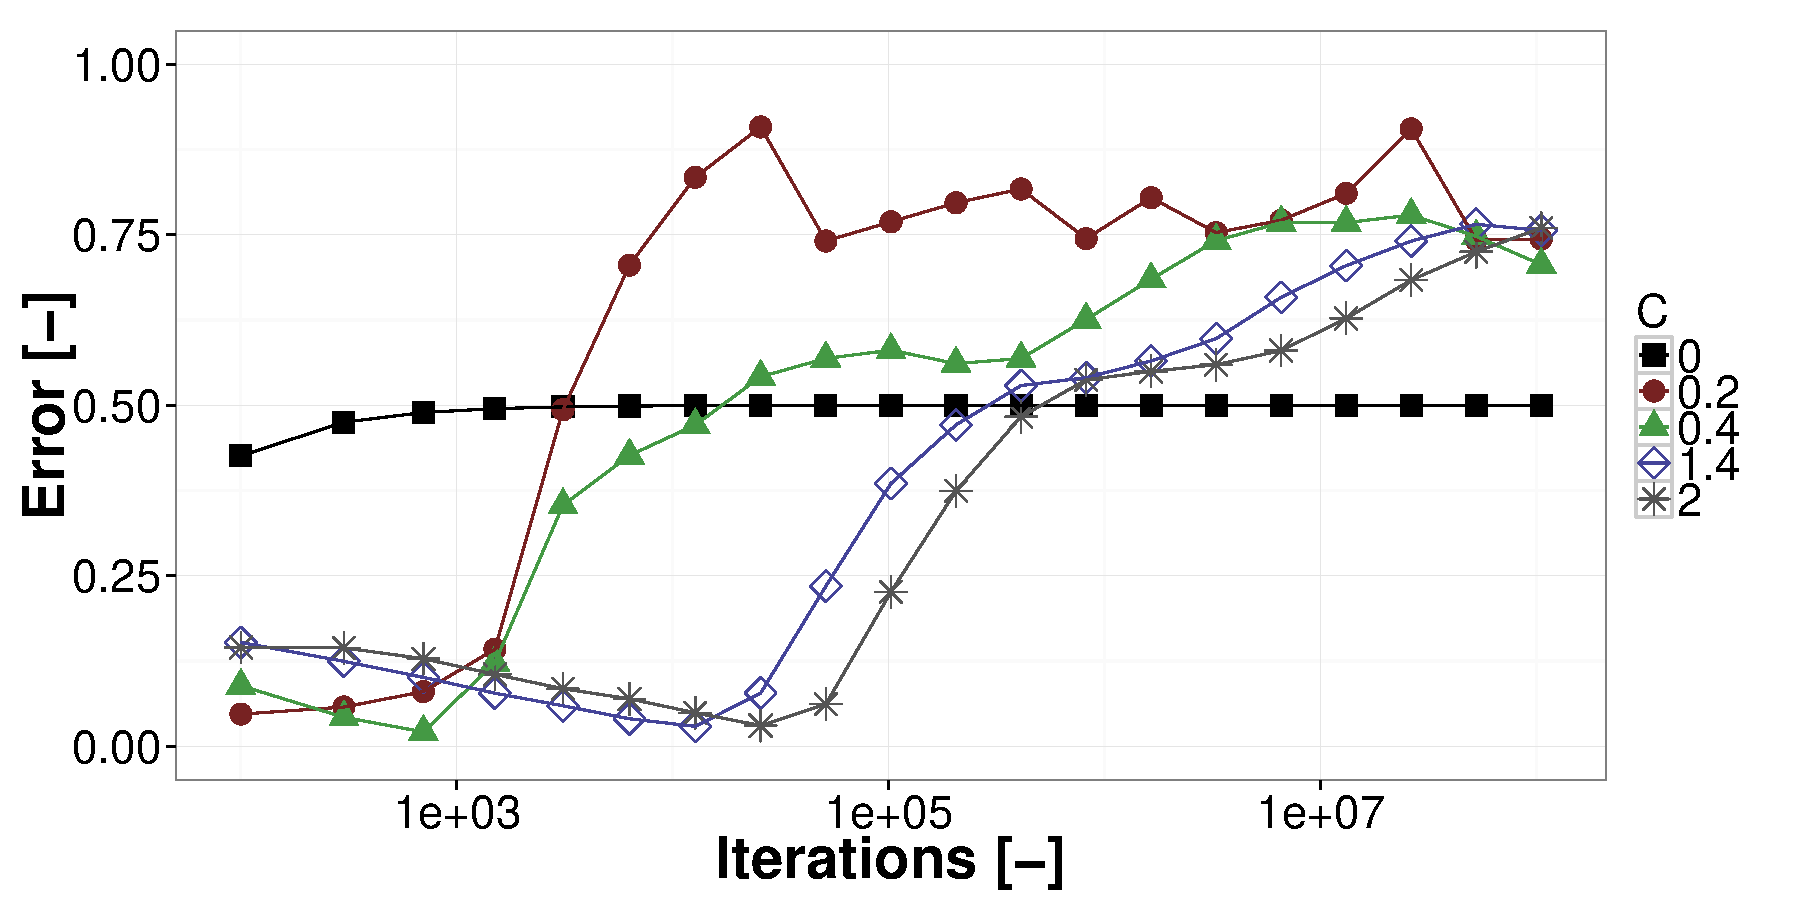
\includegraphics[width=0.8\textwidth]{figures/brps-MCTS-UCT.pdf} \\
{\small MCTS-UCT with stochastic tie-breaking} \\
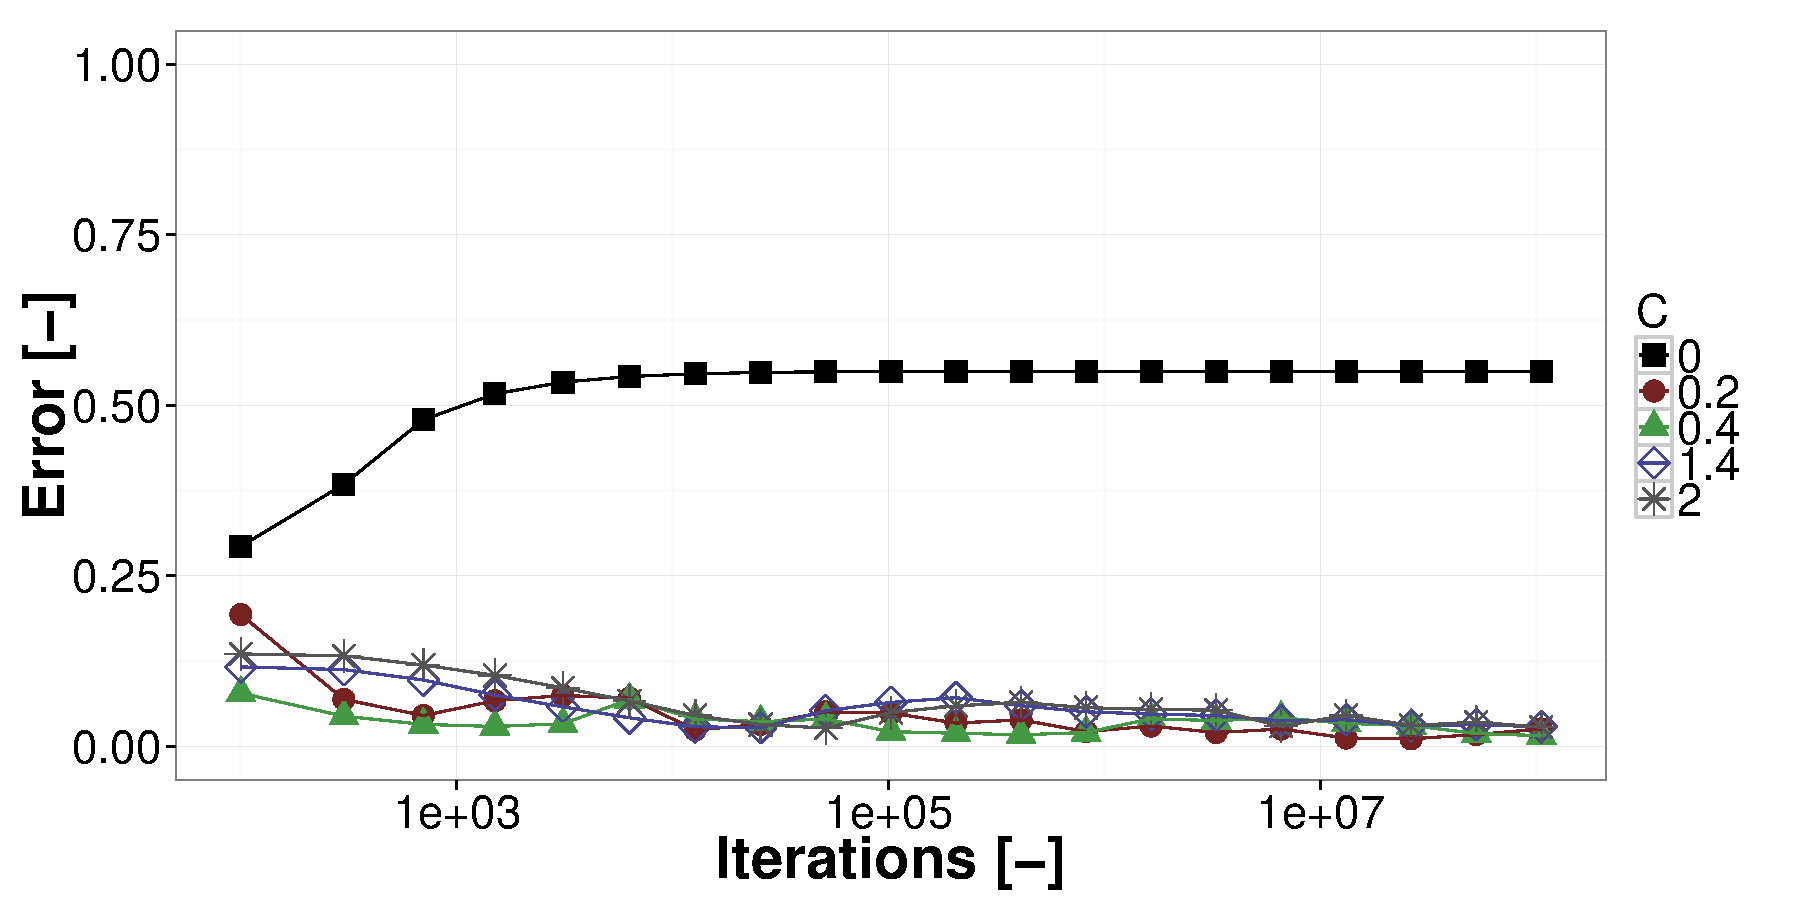
\includegraphics[width=0.8\textwidth]{figures/brps-MCTS-UCT-NONDET.pdf} \\
\end{tabular}
\caption{Exploitability of strategies of recommended by MCTS-UCT over time in Biased Rock, Paper, Scissors. Vertical axis represents exploitability. }
\label{fig:expl-brps1}
\end{figure}

\begin{figure}[t!]
\centering
\begin{tabular}{c}
%{\small MCTS-UCT (fully deterministic)} \\
%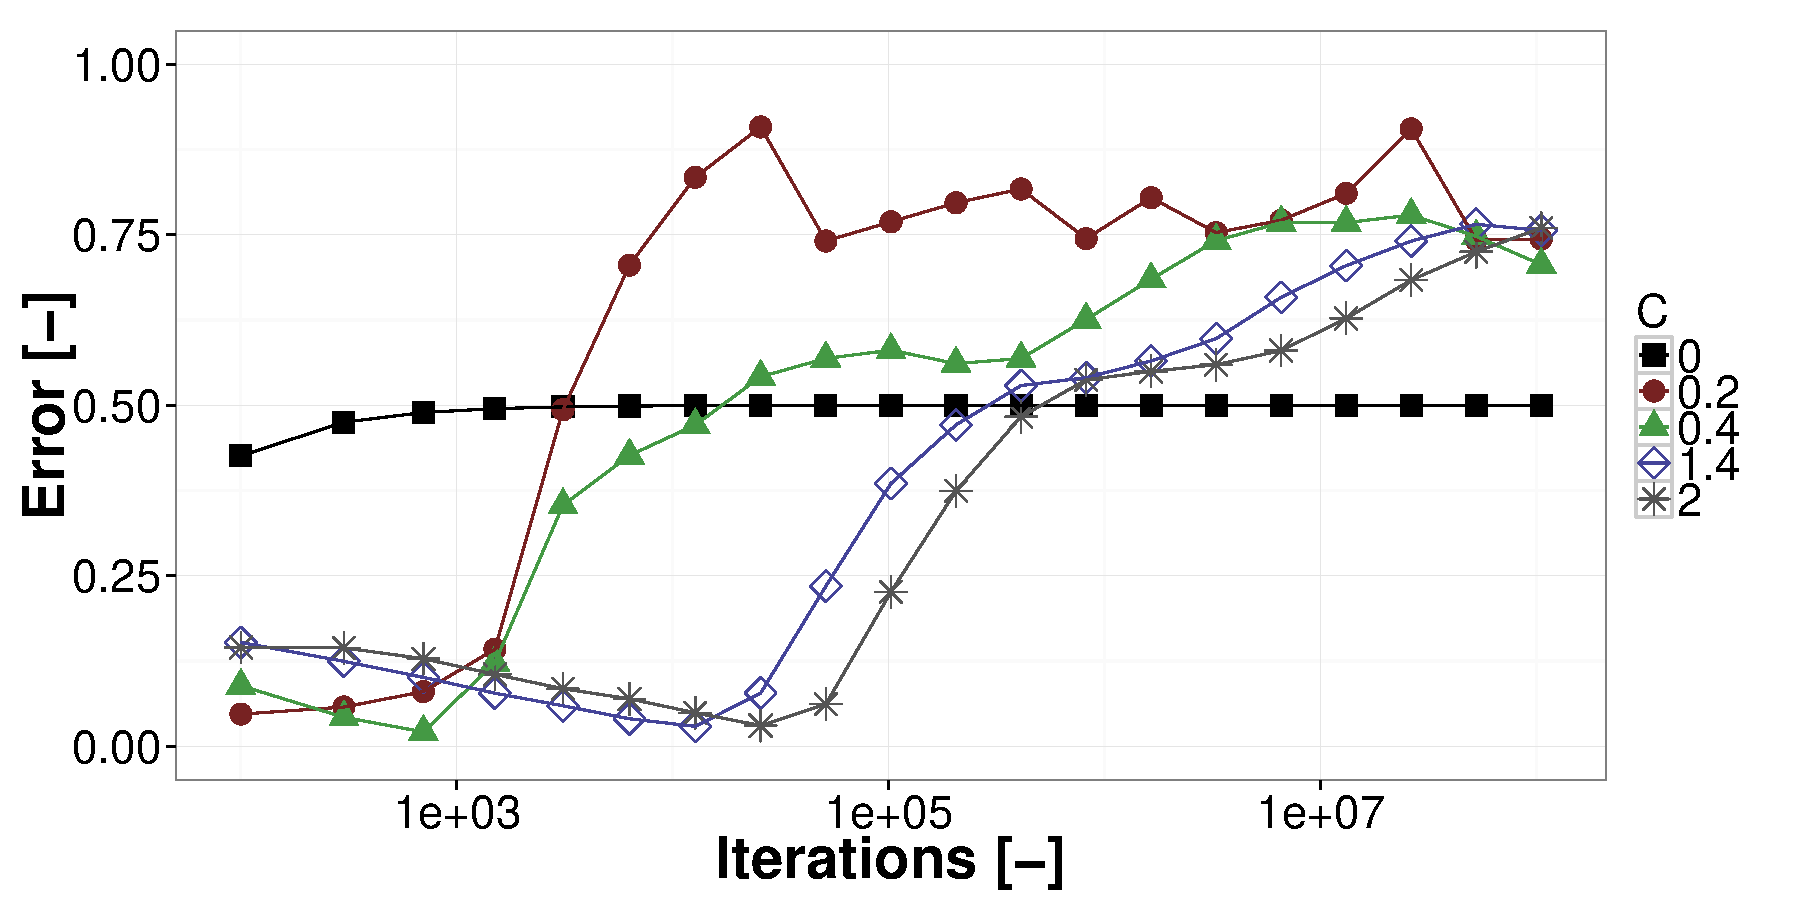
\includegraphics[width=0.4\textwidth]{figures/brps-MCTS-UCT.pdf} \\
%{\small MCTS-UCT with stochastic tie-breaking} \\
%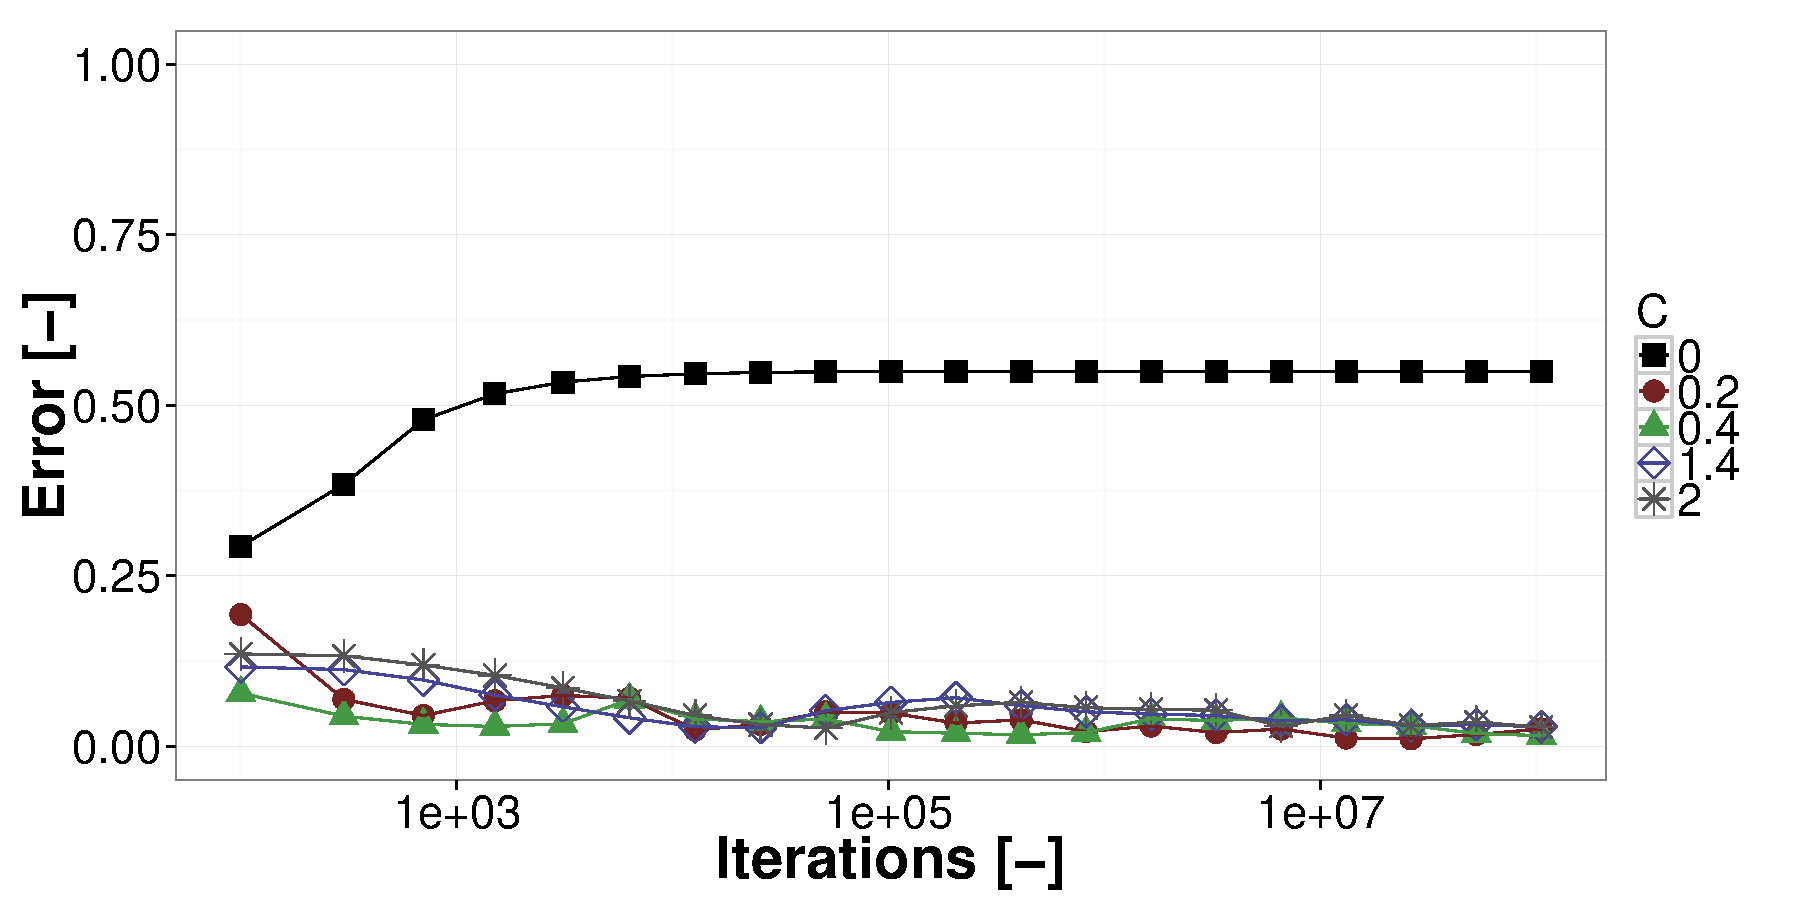
\includegraphics[width=0.4\textwidth]{figures/brps-MCTS-UCT-NONDET.pdf} \\
{\small MCTS-Exp3} \\
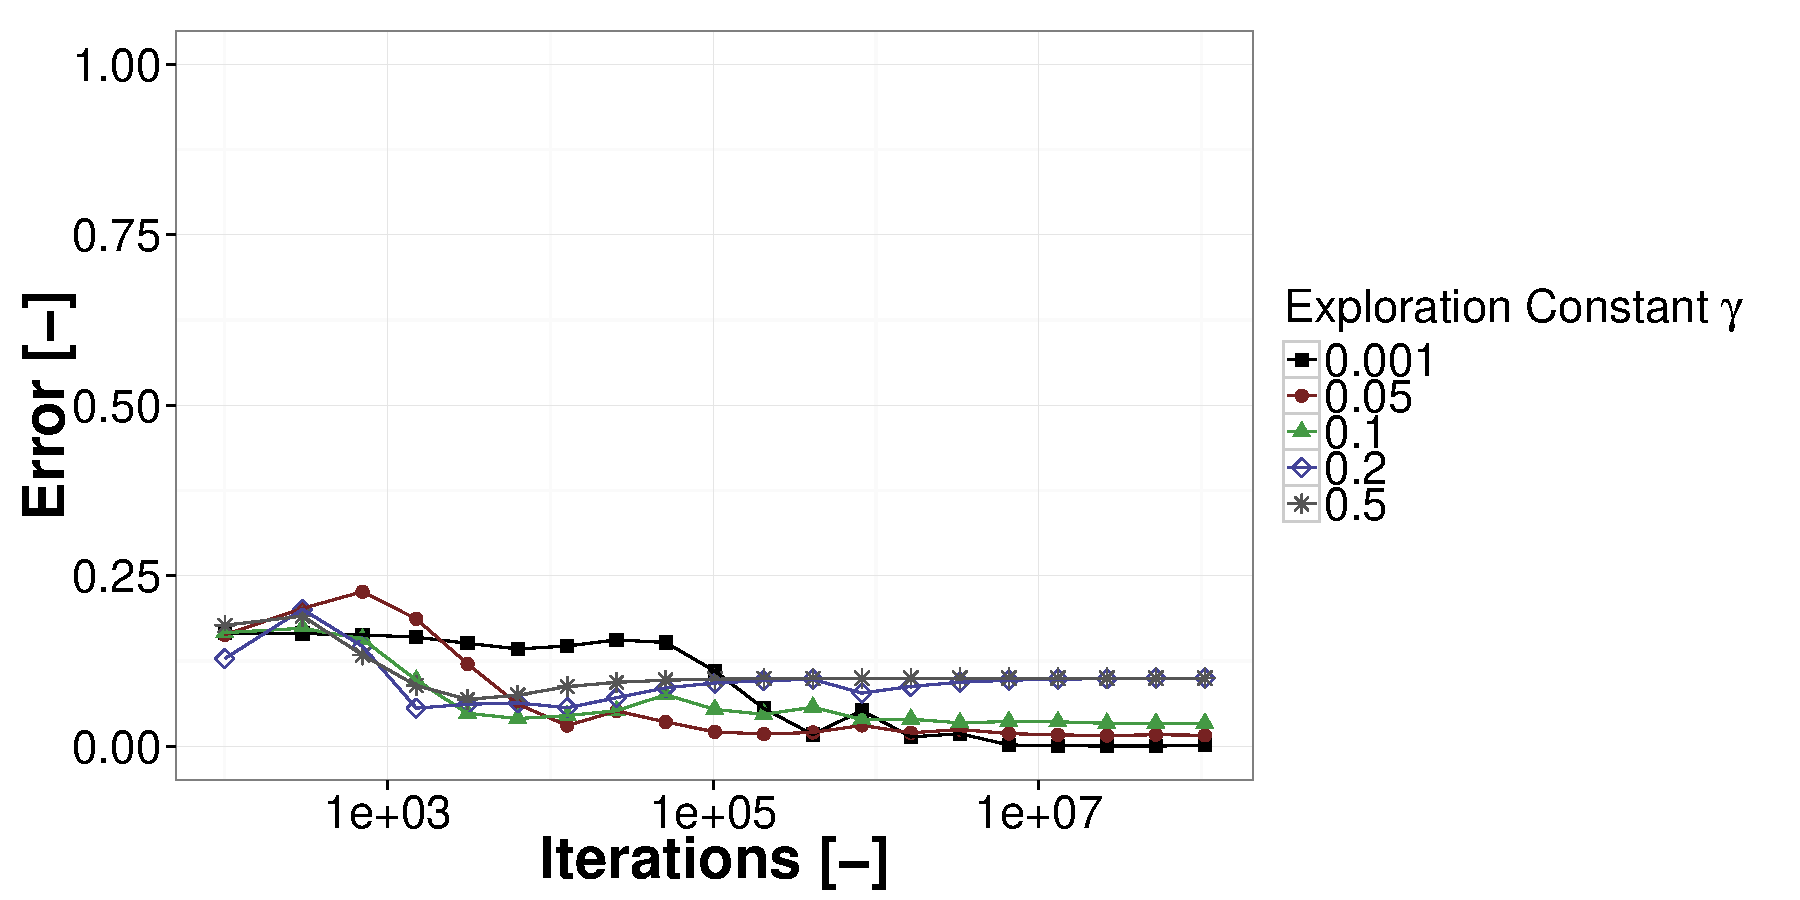
\includegraphics[width=0.8\textwidth]{figures/brps-MCTS-EXP3.pdf} \\
{\small MCTS-RM} \\
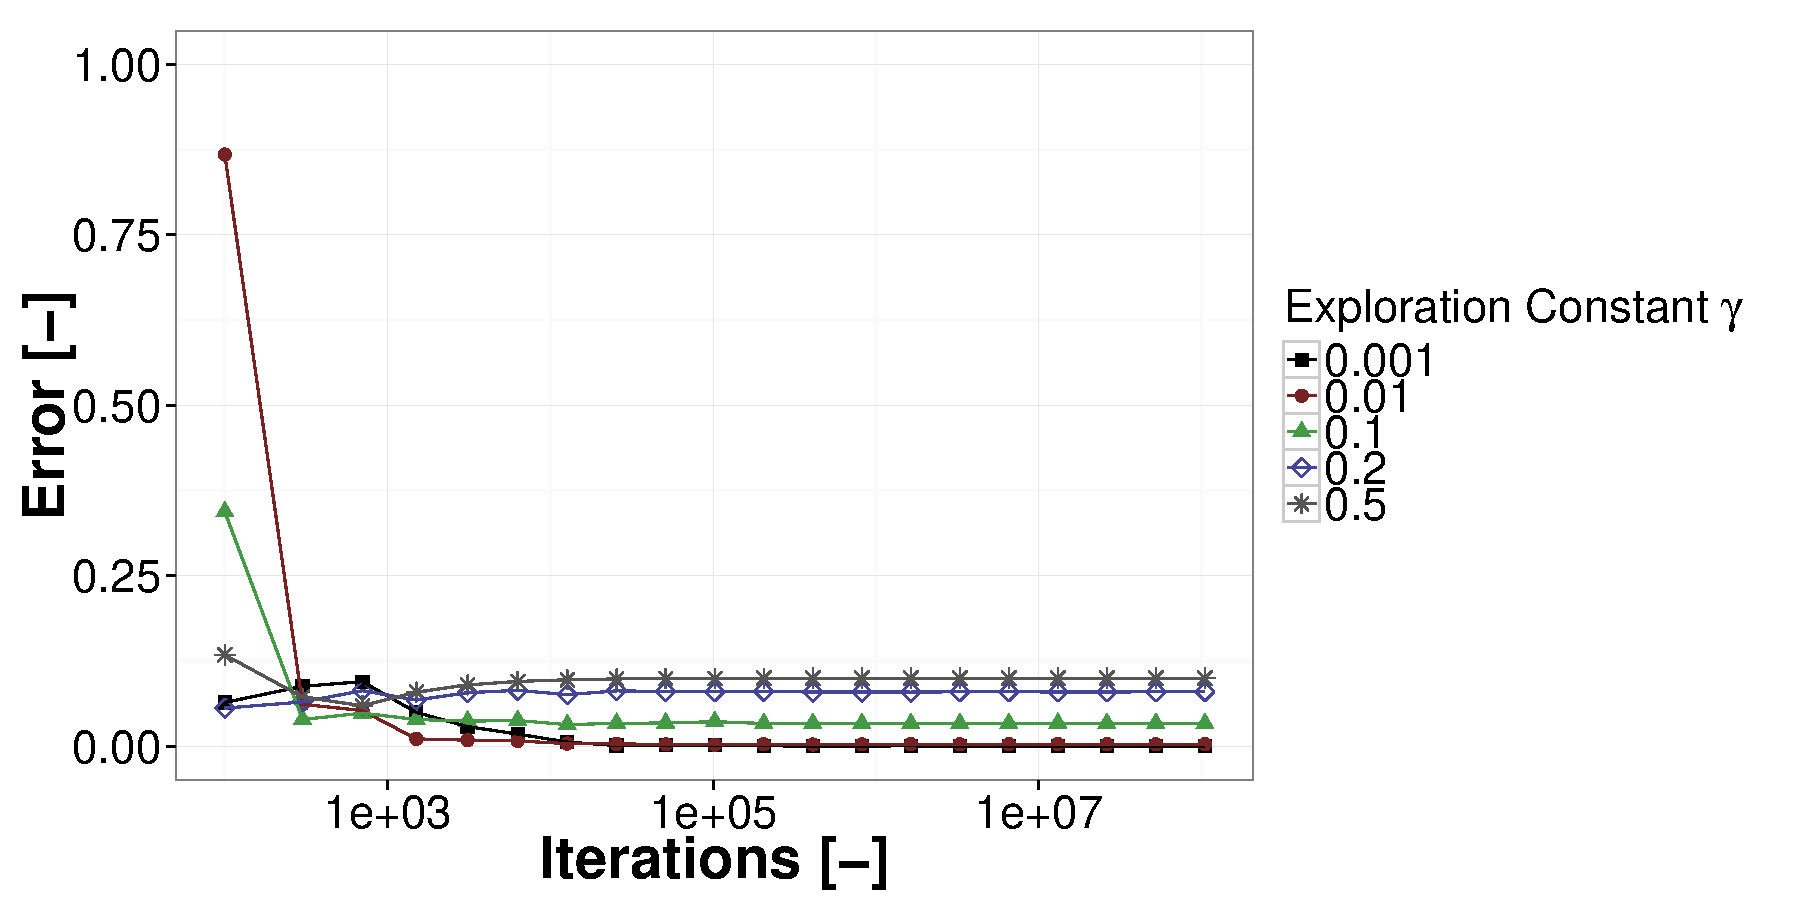
\includegraphics[width=0.8\textwidth]{figures/brps-MCTS-RM.pdf} \\
\end{tabular}
\caption{Exploitability of strategies of recommended by MCTS-Exp3 and MCTS-RM over time in Biased Rock, Paper, Scissors. Vertical axis represents exploitability. }
\label{fig:expl-brps2}
\end{figure}

We then tried adding a stochastic tie-breaking rule to the UCT selection mechanism typically used in MCTS implementations, which chooses an
action randomly when the scores of the best values are ``tied'' (less than $0.01$ apart).
Figure~\ref{fig:expl-brps1}, bottom figure shows the convergence.
One particularly striking observation is that this simple addition leads to a large drop in resulting exploitability, where exploitability
ranges from $[0.5,0.8]$ in the deterministic case, compared to $[0.01,0.05]$ with stochastic tie-breaking. Therefore, stochastic tie-breaking is
enabled in all of our experiments.

In summary, with this randomization UCT appears to be converging to an approximate equilibrium but not to an
exact equilibrium, which is similar to results of UCT in Kuhn poker~\cite{Ponsen11Computing}.

%mlanctot: is this true? %bbosansky: yes, we have run again experiments with randomized uct where deterministic uct had been used before

%\mlanctot{I noticed Vilo added his example to the SM-MCTS section so please modify this paragraph as necessary. Maybe it can be
%removed entirely?} We investigated this further and found a possible
%explanation of this behavior. Consider the matrix game on the right of Figure~\ref{fig:egMatrixGames} in Section~\ref{sec:smg}.
%Suppose DUCT is run on this game and players deterministically prefer the left-action.
%DUCT will always recieve rewards 0 and the exploration bias term will cause the players to round-robin over the actions indefinitely.
%However, each player can than improve by playing first action with probability 1. Breaking ties stochastically will lead the algorithm to
%discover the 1 and -1 rewards with high probability and allow the algorithm the break out or avoid this synchronization trap.

\subsection{Offline Equilibrium Computation} \label{sec:eval:offline}

We now compare the offline performance of the algorithm on all the remaining games.
We measure the overall computation time for each of the algorithms and number of evaluated nodes -- \ie nodes for which the main method of the backward induction algorithm executed (\ie nodes evaluated by serialized alpha-beta algorithms are not included in this count, since they may be evaluated repeatedly).
Unless otherwise stated, each data point represents a mean of at least $30$ runs.
% mlanctot: check this %bbosansky: ?

\subsubsection{Goofspiel}
\begin{figure} [t]
\centering
	\begin{subfigure}{0.49\textwidth}
 		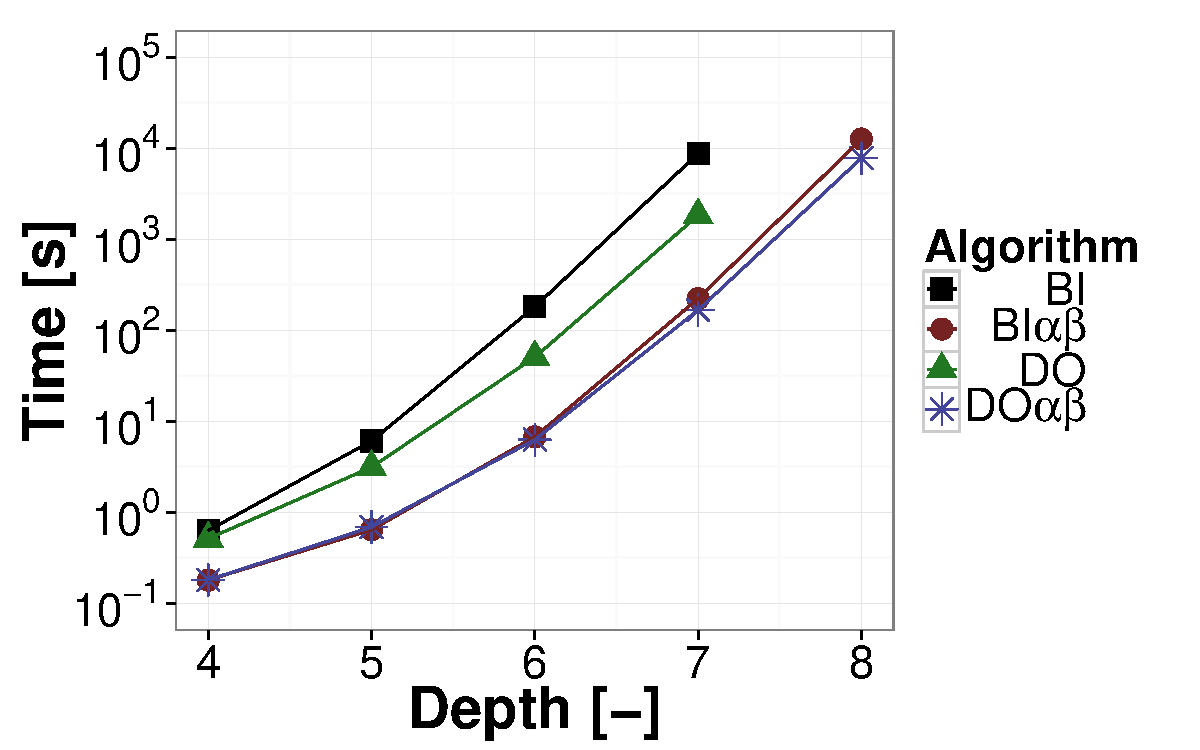
\includegraphics[width=1\textwidth]{figures/GS-BT-NF.pdf}\caption{}\label{fig:off:res:gs-bt}
 	\end{subfigure}
	\begin{subfigure}{0.49\textwidth}
 		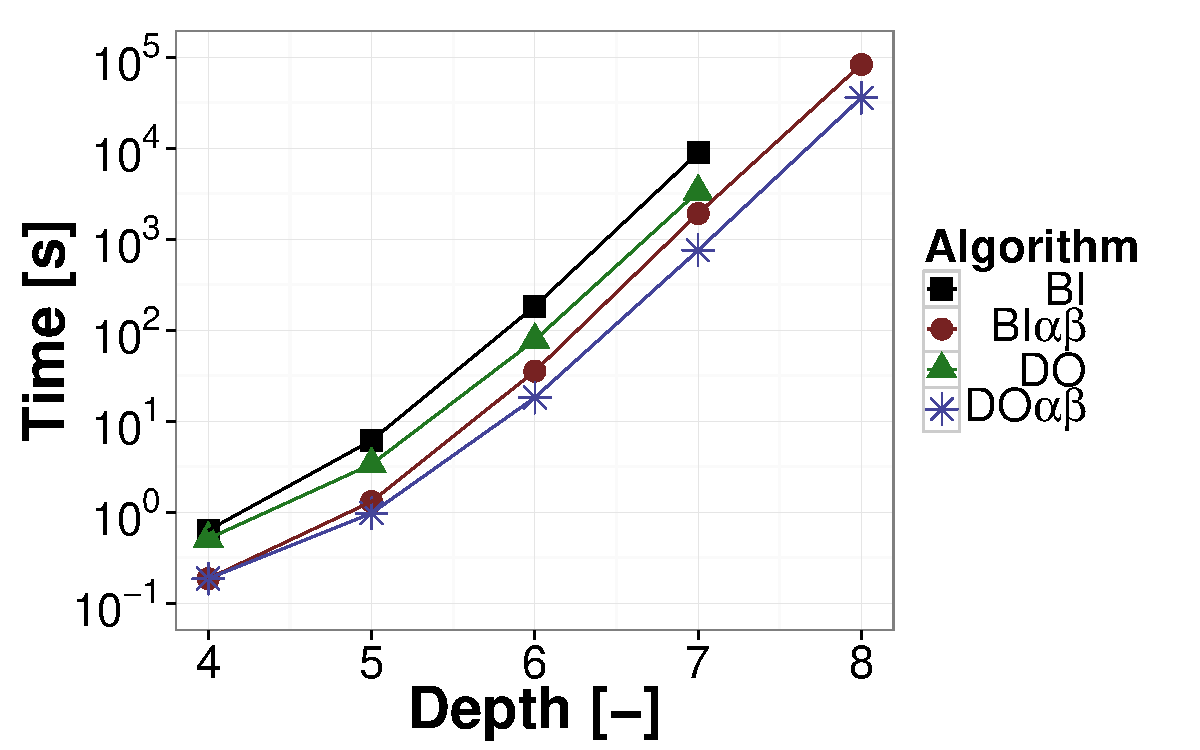
\includegraphics[width=1\textwidth]{figures/GS-BF-NF.pdf}\caption{}\label{fig:off:res:gs-bf}
 	\end{subfigure}
\caption{Running times of exact algorithms on Goofspiel with fixed order of the nature's cards for increasing size of the deck; subfigure (a) depicts the results with win-tie-loose utilities, (b) depicts the results with point utilities.} \label{fig:off:res:gs}
\end{figure}

We now describe the results for the card game Goofspiel.
First, we analyze the games with a fixed ordering of the cards by nature.

\paragraph{Exact algorithms with fixed ordering}
The results are depicted in Figure~\ref{fig:off:res:gs} (note the logarithmic vertical scale), where the left subfigure depicts the results for win-tie-loose utilities and the right subfigure depicts the results for point utilities.
The comparison on the win-tie-loose variant shows that there is a significant number of subgames with pure Nash equilibrium that can be computed using serialized alpha-beta algorithms.
Therefore, the performance of $\biab$ and $\doab$ is fairly similar and the gap only slowly increases in favor of $\doab$ with the increasing size of the game.
Since serialized alpha-beta is able to solve a large portion of subgames, both of these algorithms significantly reduce the number of the states visited by the backward induction algorithm.
While \textsc{BI} algorithm evaluates than $3.2\times10^7$ nodes in the setting with $7$ cards in more than $2.5$ hours, $\biab$ evaluates only $198,986$ nodes in less than $4$ minutes.
The performance is further improved by $\doab$ that evaluates on average $79,105$ nodes in less than $3$ minutes.
The overheads are slightly higher in case of $\doab$; hence, the time difference between $\doab$ and $\biab$ is relatively small compared to the difference in evaluated nodes.
Finally, the results show that even simple \textsc{DO} algorithm without serialized alpha-beta search can improve the performance of \textsc{BI}.
In the setting with $7$ cards, \textsc{DO} evaluates more than $6\times10^6$ nodes which takes on average almost 30 minutes.

\reviewchange{The results for the point utilities are the same for BI, while DO is slightly worse.
On the other hand, the success of serialized alpha-beta algorithm is significantly lower and it takes both algorithms much more time to solve games of same size.
With $7$ cards, $\biab$ now evaluates more than $2\times10^6$ nodes and it takes the algorithm on average $32$ minutes to find the solution.
$\doab$ is still the fastest and it evaluates more than $3\times10^5$ nodes in less than $13$ minutes on average.}

The performance of algorithms $\biab$ and $\doab$ represent a significant improvement over the results of the pruning algorithm
SMAB presented in \cite{Saffidine12SMAB}.
In their work, the number of evaluated nodes was at best around $29\%$, and the running time improvement was only marginal.

\reviewchange{
\paragraph{Exact algorithms with chance nodes}

\begin{figure}[t]
\centering
	\begin{subfigure}{0.49\textwidth}
 		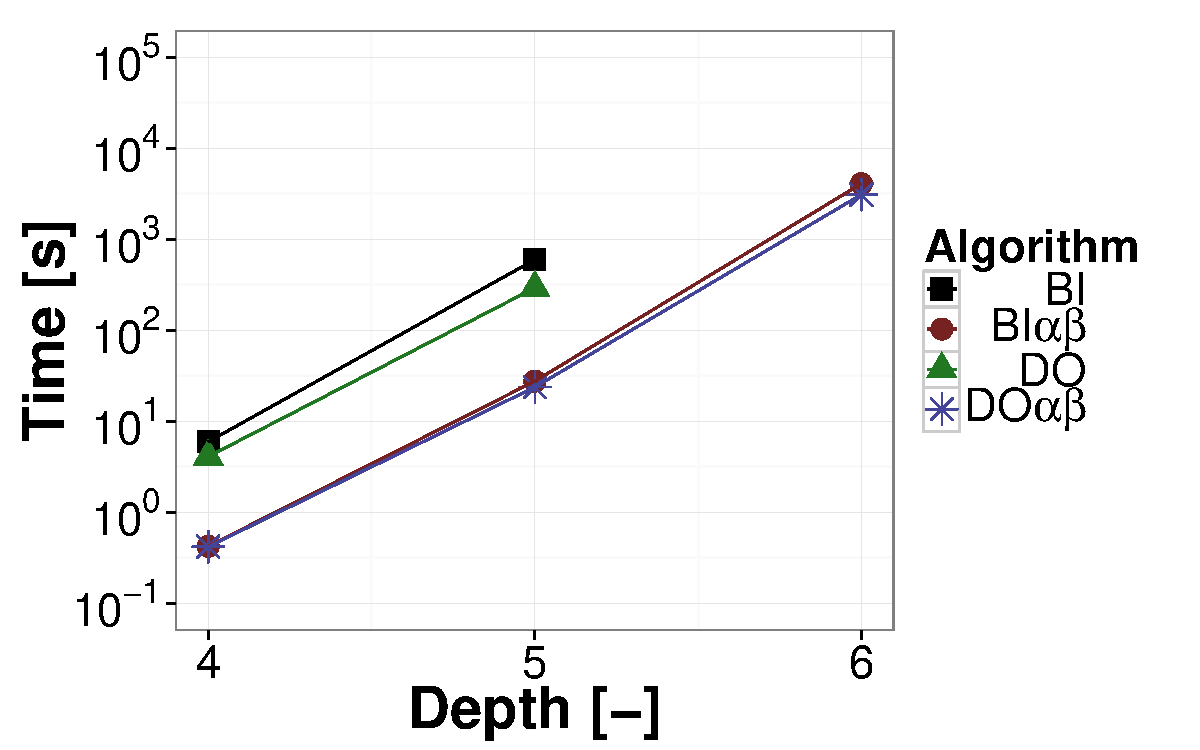
\includegraphics[width=1\textwidth]{figures/GS-BT-NN.pdf}\caption{}\label{fig:off:res:gsn-bt}
 	\end{subfigure}
	\begin{subfigure}{0.49\textwidth}
 		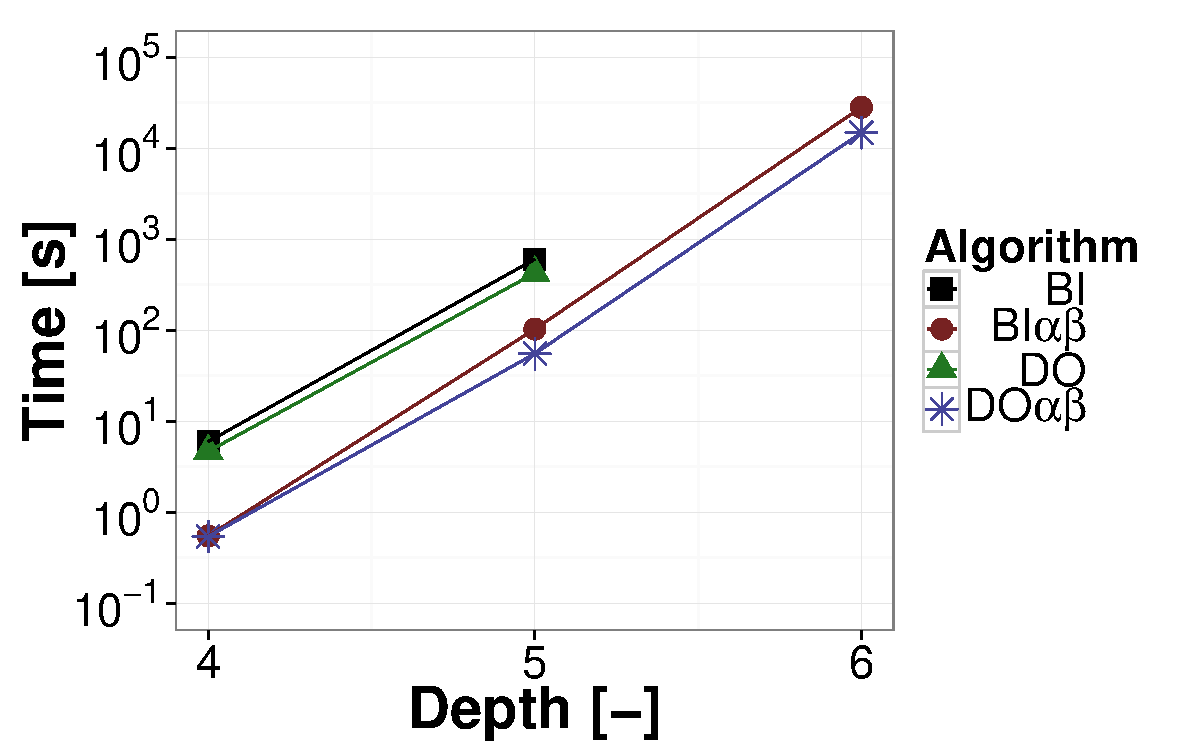
\includegraphics[width=1\textwidth]{figures/GS-BF-NN.pdf}\caption{}\label{fig:off:res:gsn-bf}
 	\end{subfigure}
\caption{Running times of exact algorithms on Goofspiel with chance nodes for increasing size of the deck; subfigure (a) depicts the results with win-tie-loose utilities, (b) depicts the results with point utilities.} \label{fig:off:res:gsn}
\end{figure}

Next we compare the exact algorithms in the variant of Goofspiel with standard chance nodes.
Introducing another branching due to moves by nature causes a significant increase in the size of the game tree.
For $7$ cards, the game tree has more than $10^{11}$ nodes, which is $4$ orders of magnitude more than in the case with fixed ordering of nature's cards.
The results depicted in Figure~\ref{fig:off:res:gsn} show that the games become quickly too large to solve exactly and the fastest algorithms solved games with at most $6$ cards.
Relative performance of the algorithms, however, is similar to the case with fixed ordering.
With win-tie-loose utilities, serialized alpha-beta is again able to find pure NE in most of the subgames and prunes out a large fraction of the states.
For the game with $5$ cards, BI evaluates more than $2 \times 10^6$ nodes in almost $10$ minutes, while $\biab$ evaluates only $17,315$ nodes in $27$ seconds and $\doab$ evaluates $6,980$ nodes in $23$ seconds.
As before, serialized alpha-beta algorithm is less helpful in the case with point utilities.
Again with $5$ cards, $\biab$ evaluates $91,419$ nodes in more than $100$ seconds and $\doab$ evaluates $14,536$ nodes in almost $55$ seconds.
}

\paragraph{Sampling algorithms with fixed ordering}

\begin{figure}[t]
	\begin{subfigure}{1\textwidth}
		\centering
		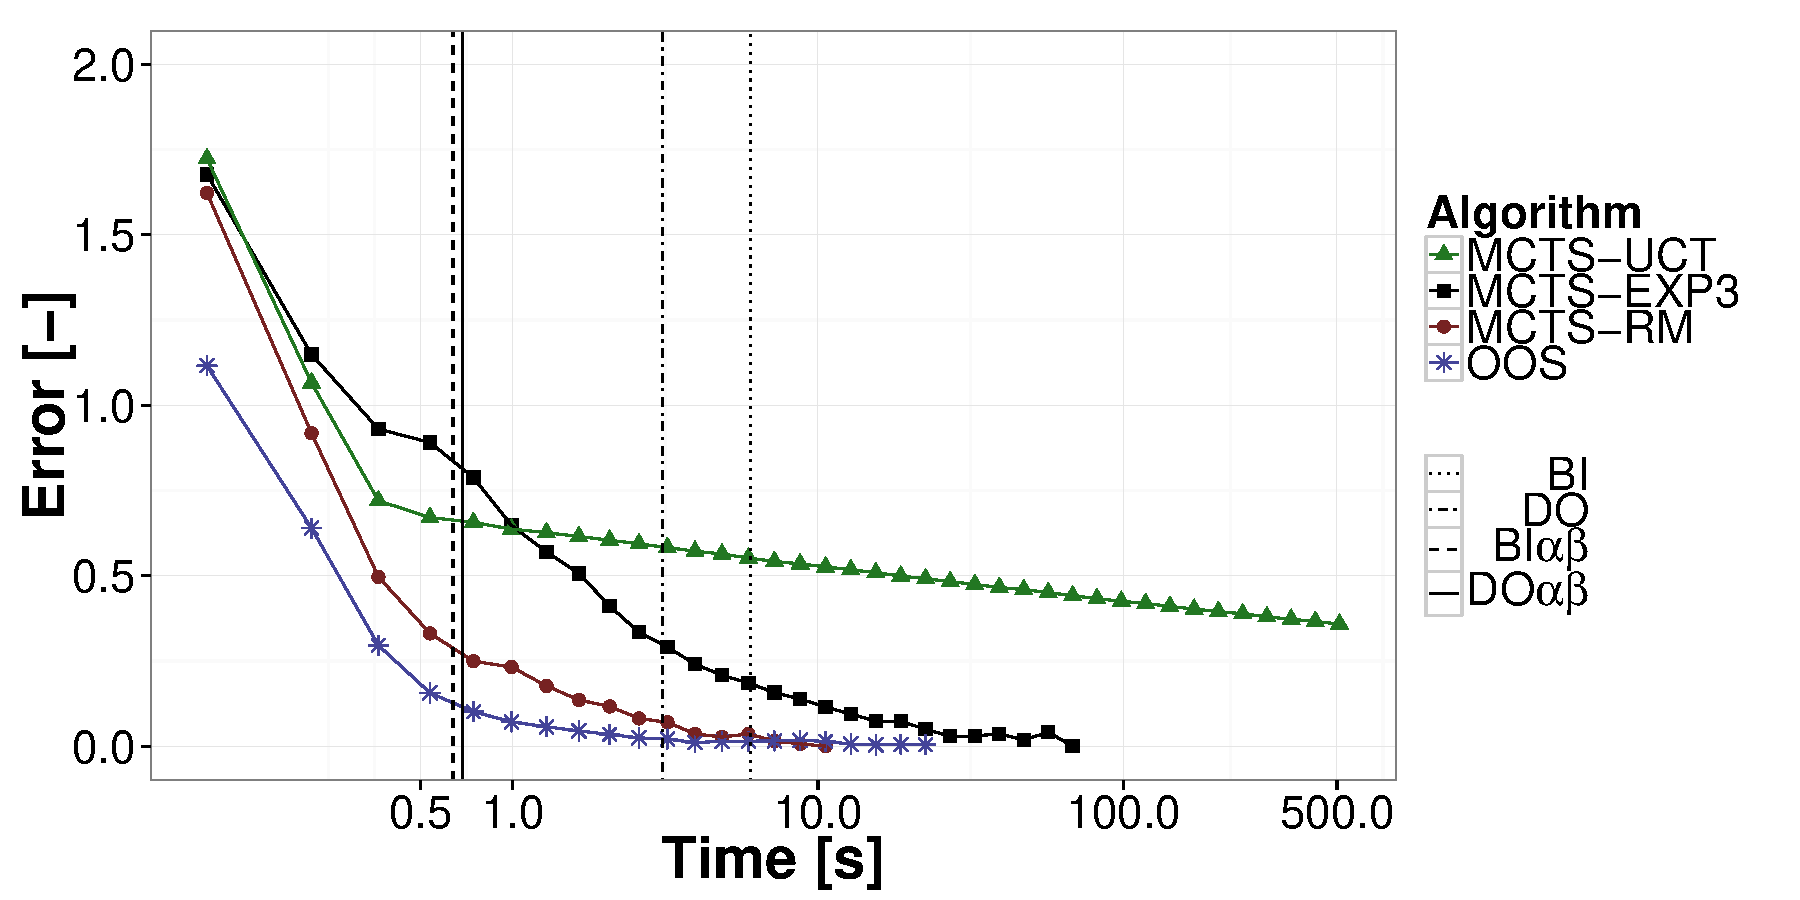
\includegraphics[width=0.85\textwidth]{figures/convergence-gs-tf.pdf}%\caption{}\label{fig:off:conv:gs-bt}
	\end{subfigure}
	\begin{subfigure}{1\textwidth}
		\centering
		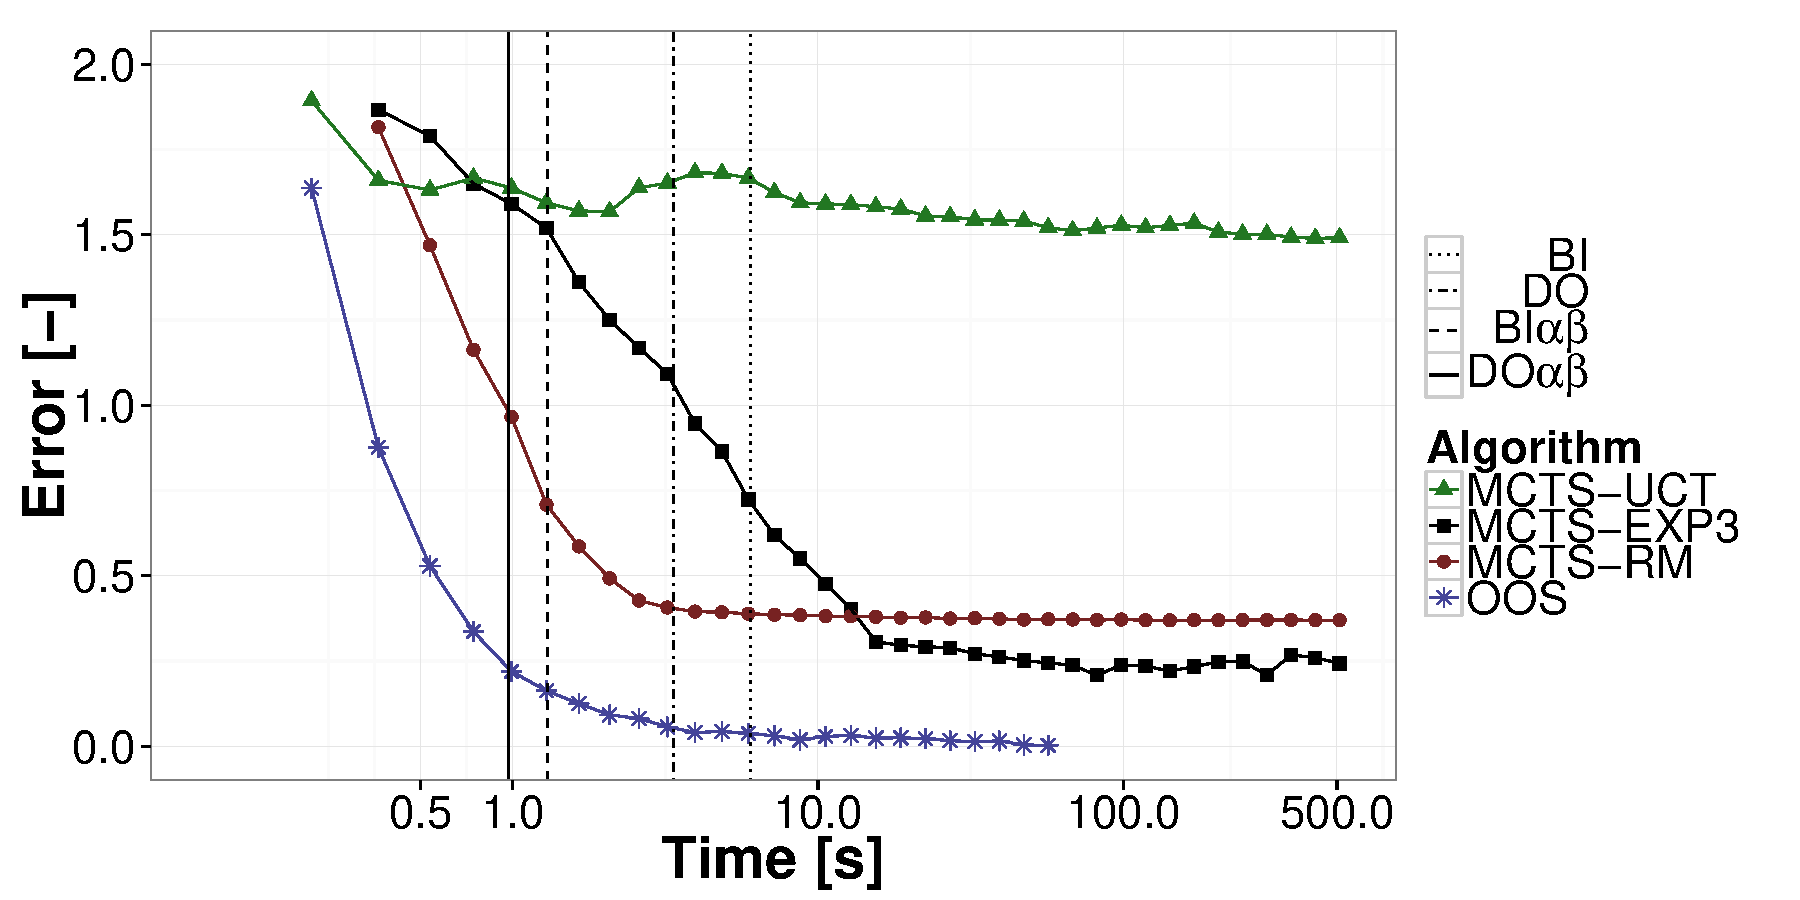
\includegraphics[width=0.85\textwidth]{figures/convergence-gs-ff.pdf}%\caption{}\label{fig:off:conv:gs-bf}
	\end{subfigure}
\caption{Convergence of sampling algorithms on Goofspiel with $5$ cards and fixed ordering of nature's cards.
Vertical lines correspond to computation times for exact algorithms.
(Top) Goofspiel with win-tie-loose utility values;
(Bottom) Goofspiel with point utilities.} \label{fig:off:conv:gs}
\end{figure}

We now turn to the analysis of the convergence of the sampling algorithms -- \ie their ability to approximate Nash equilibrium strategies of the complete game.
Figure~\ref{fig:off:conv:gs} depicts the results for Goofspiel game with $5$ cards with fixed ordering cards of nature (note the logarithmic horizontal scale).
We compare MCTS algorithms with three different selection functions (UCT, Exp3, and RM), and OOS.
The results are means out of $30$ runs of each algorithm.
Due to the different selection and update functions, the algorithms differ in the number of iterations per second.
RM is the fastest with more than $2.6\times 10^5$ iterations per second, OOS has around $2\times10^5$ iterations, UCT $1.9\times10^5$, and Exp3 only $5.4\times10^4$ iterations.

The results show that OOS converges the fastest out of all sampling algorithms.
This is especially noticeable in the point-utility settings, where none of the other sampling algorithms were approaching zero error due to the exploration.
MCTS with RM selection function is only slightly slower in the win-tie-loose case, however, other two selection functions perform worse.
While Exp3 eventually converges close to $0$ in the win-tie-loose case, the exploitability of UCT decreases rather slowly and it was still over $0.35$ at the time limit of $500$ seconds.
The best $C$ constant for UCT was 5 in win-tie-loose setting, and $10$ in the point utility setting.
While setting lower constant typically improved slightly the
convergence during the first iterations, the final error was always larger.
%Moreover, when we have not used randomization in UCT, the algorithm was not able to converge to error lower than $0.5$ in the time limit.
%On the other hand, both OOS and RM confirm their quick convergence, witch is aligned with previous results~\cite{Lanctot13Goofspiel}.
The vertical lines represent times for exact algorithms.
In the win-tie-loose case, $\biab$ is slightly faster and finishes first in $0.64$ second, followed by $\doab$ ($0.69$ seconds), \textsc{DO} ($3.1$ seconds), and \textsc{BI} ($6$ seconds).
In the point case, $\doab$ is the fastest ($0.97$ seconds), followed by $\biab$ ($1.3$ seconds), followed by \textsc{DO} and \textsc{BI} with similar times as in the previous case.

\reviewchange{
\paragraph{Sampling algorithms with chance nodes}

\begin{figure}[t]
	\begin{subfigure}{1\textwidth}
		\centering
		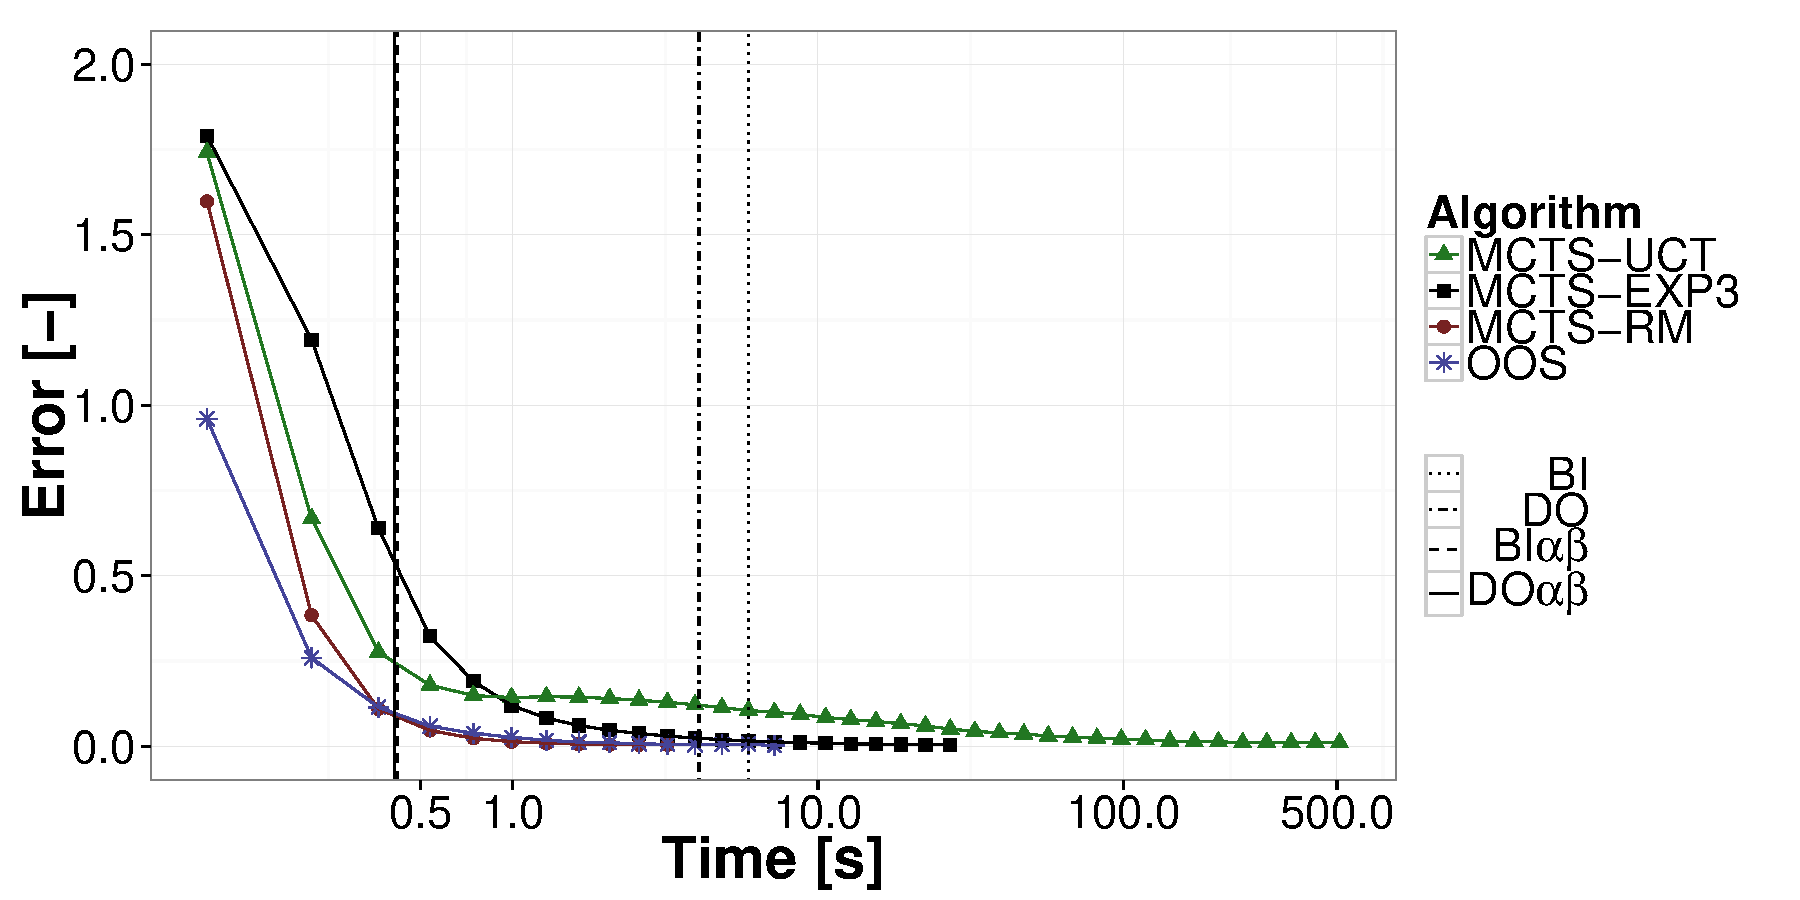
\includegraphics[width=0.85\textwidth]{figures/convergence-gs-tn.pdf}%\caption{}\label{fig:off:conv:gs-bt}
	\end{subfigure}
	\begin{subfigure}{1\textwidth}
		\centering
		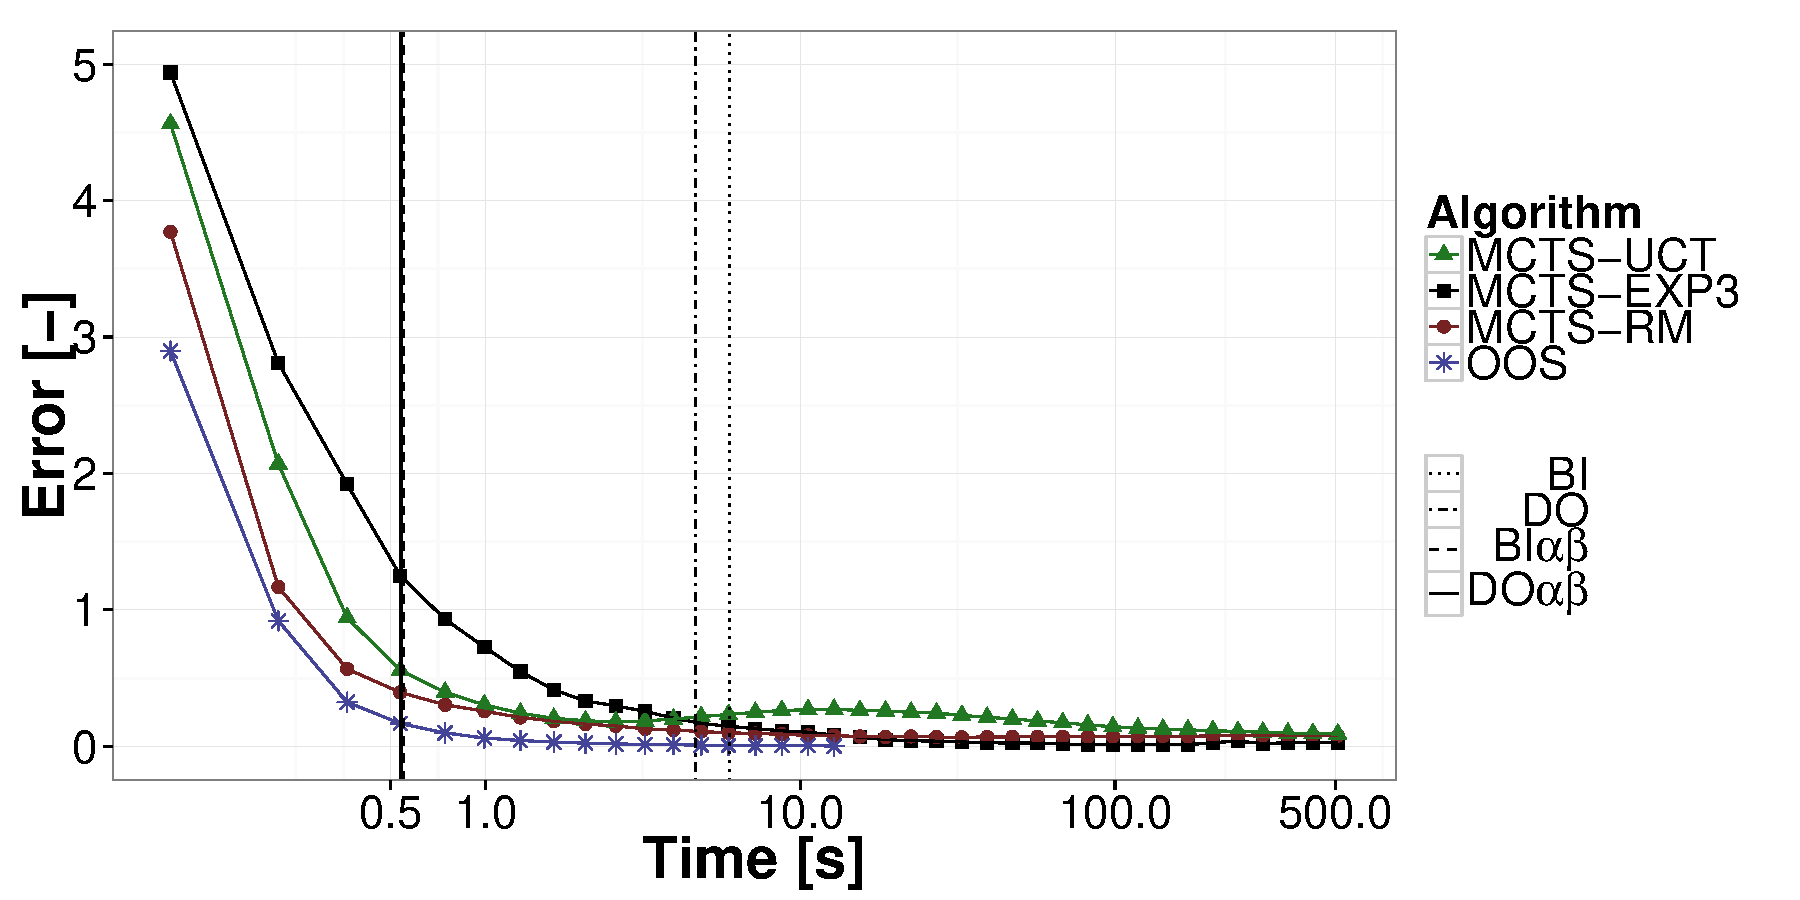
\includegraphics[width=0.85\textwidth]{figures/convergence-gs-fn.pdf}%\caption{}\label{fig:off:conv:gs-bf}
	\end{subfigure}
\caption{Convergence of sampling algorithms on Goofspiel with $4$ cards and chance nodes.
Vertical lines correspond to computation times of exact algorithms.
(Top) Goofspiel with win-tie-loose utility values;
(Bottom) Goofspiel with point utilities.} \label{fig:off:conv:gsn}
\end{figure}

We also performed the experiments in the setting with chance nodes.
Due to the size of the game tree, we have reduced the number of cards to $4$, since the size of this game tree is comparable to the case with $5$ cards and fixed ordering of cards.
The results depicted in Figure~\ref{fig:off:conv:gsn} show a similar behavior of the sampling algorithms as we have observed in the previous case.
OOS converges the fastest, followed by RM, and EXP3.
Main difference is in the convergence of UCT, however, this is mostly due to the fact that pure NE exists in Goofspiel with 4 cards; hence, UCT can better identify the best action to play and converges more quickly to less exploitable strategy than in the case with 5 cards.
Surprisingly, the convergence of the algorithms does not change that dramatically with the introduction of point utilities as in the previous case.
The main reason is that the range of the utility values is smaller compared to the previous case (there is one card less in the present setting and the missing cards has the highest value).
For comparison, we again use the vertical lines to denote times of exact algorithms.
$\biab$ and $\doab$ are almost identically fast, with $\doab$ being slightly faster, followed by \textsc{DO} and \textsc{BI}.
}

\subsubsection{Pursuit-Evasion Games}
\begin{figure}
\centering
	\begin{subfigure}{0.49\textwidth}
		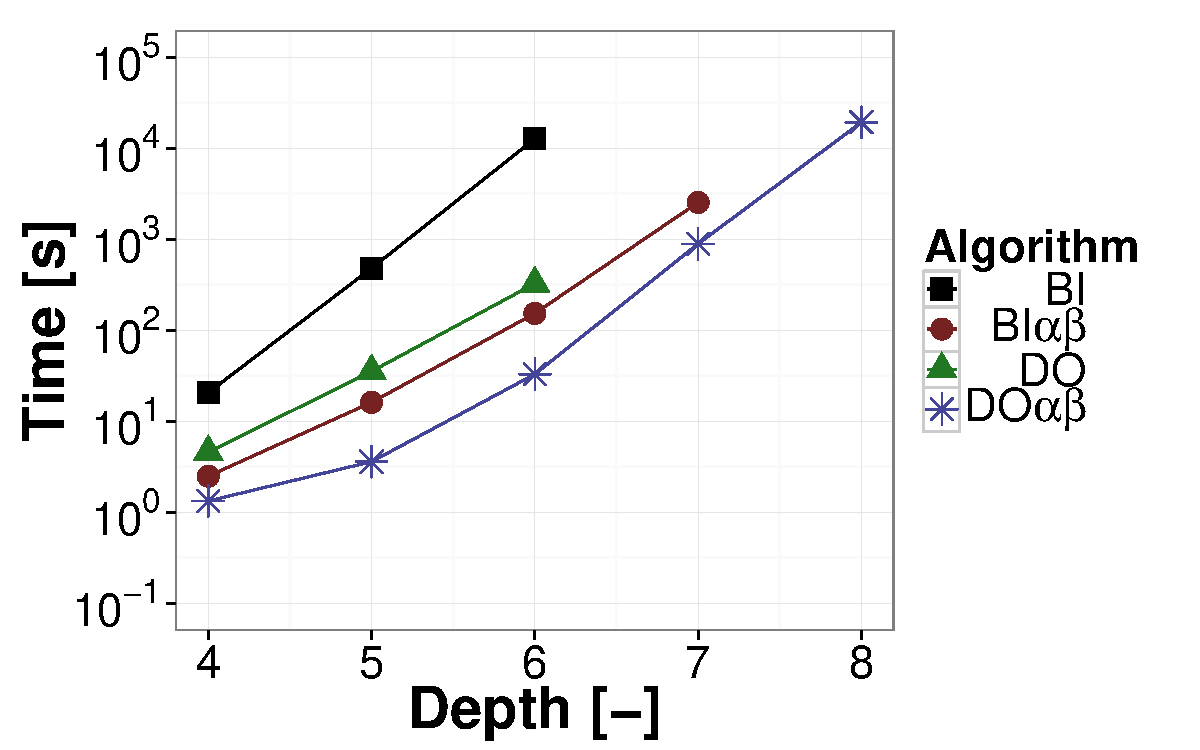
\includegraphics[width=1\textwidth]{figures/PEG4x4.pdf}\caption{}\label{fig:off:res:peg4}
	\end{subfigure}
	\begin{subfigure}{0.49\textwidth}
		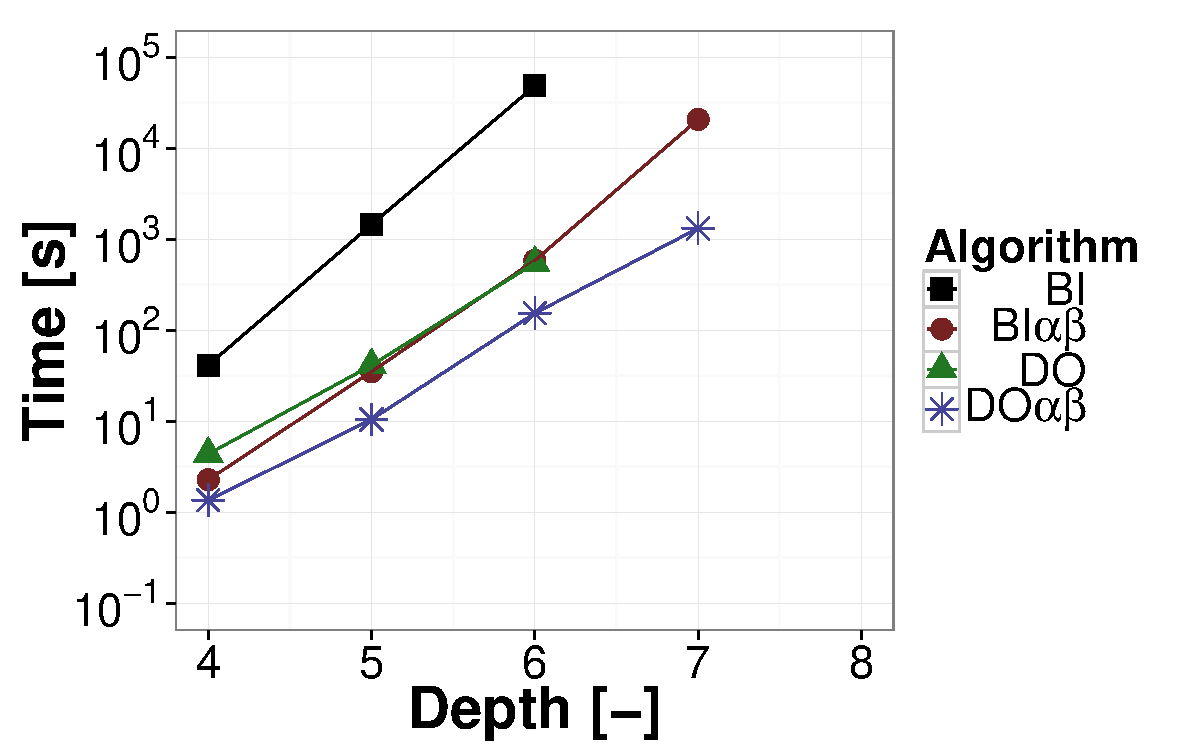
\includegraphics[width=1\textwidth]{figures/PEG5x5.pdf}\caption{}\label{fig:off:res:peg5}
	\end{subfigure}
\caption{Running times of exact algorithms on pursuit-evasion game with increasing number of moves: subfigure (a) depicts the results on $4\times4$ grid graph, (b) depicts results for $5\times5$ grid.} \label{fig:off:res:peg}
\end{figure}

The results on pursuit-evasion games show more significant improvement when comparing $\doab$ and $\biab$ (see Figure~\ref{fig:off:res:peg}). In all settings, the $\doab$ is significantly the fastest. When we compare the performance on graph $5\times5$ with depth set to $6$, \textsc{BI} evaluates more than $4.9\times10^7$ nodes that takes more than $13$ hours. On the other hand, $\biab$ evaluates on average $42001$ nodes taking almost $10$ minutes ($584$ seconds). Interestingly, the benefits of pure integration with alpha-beta search is not that helpful in this game.
This is apparent from results of \textsc{DO} algorithm that evaluates less than $2\times10^6$ nodes but it takes slightly over $9$ minutes on average ($547$ seconds). Finally, $\doab$ evaluates only $6692$ nodes and it takes the algorithm less than $3$ minutes.

Large parts of these pursuit-evasion games can be solved by serialized alpha-beta algorithms.
These parts typically corresponds to clearly winning, or clearly losing positions for a player; hence, serialized alpha-beta algorithms are able to prune substantial portion of the space.
However, since there are only two pursuit units, it is still necessary to use mixed strategies for final coordination (capturing the evader close to edge of the graph), and thus mixing strategy occurs near the end of the game tree.
Therefore, serialized alpha-beta is not able to solve all subgames, while double-oracle provides additional pruning since many of the actions in the subgames are leading to the same outcome and not all of them are required to find equilibrium strategies.
This causes additional improvement in computation time for $\doab$ compared to $\biab$ and all the other algorithms.%\vlisy{This argument is not very consistent with $\biab$ evaluating $\tfrac{1}{1000}$ of the nodes BI evaluates, while DO evaluating $\tfrac{1}{20}$. The reason is likely the cost of serialized searches.}

\begin{figure}
\centering
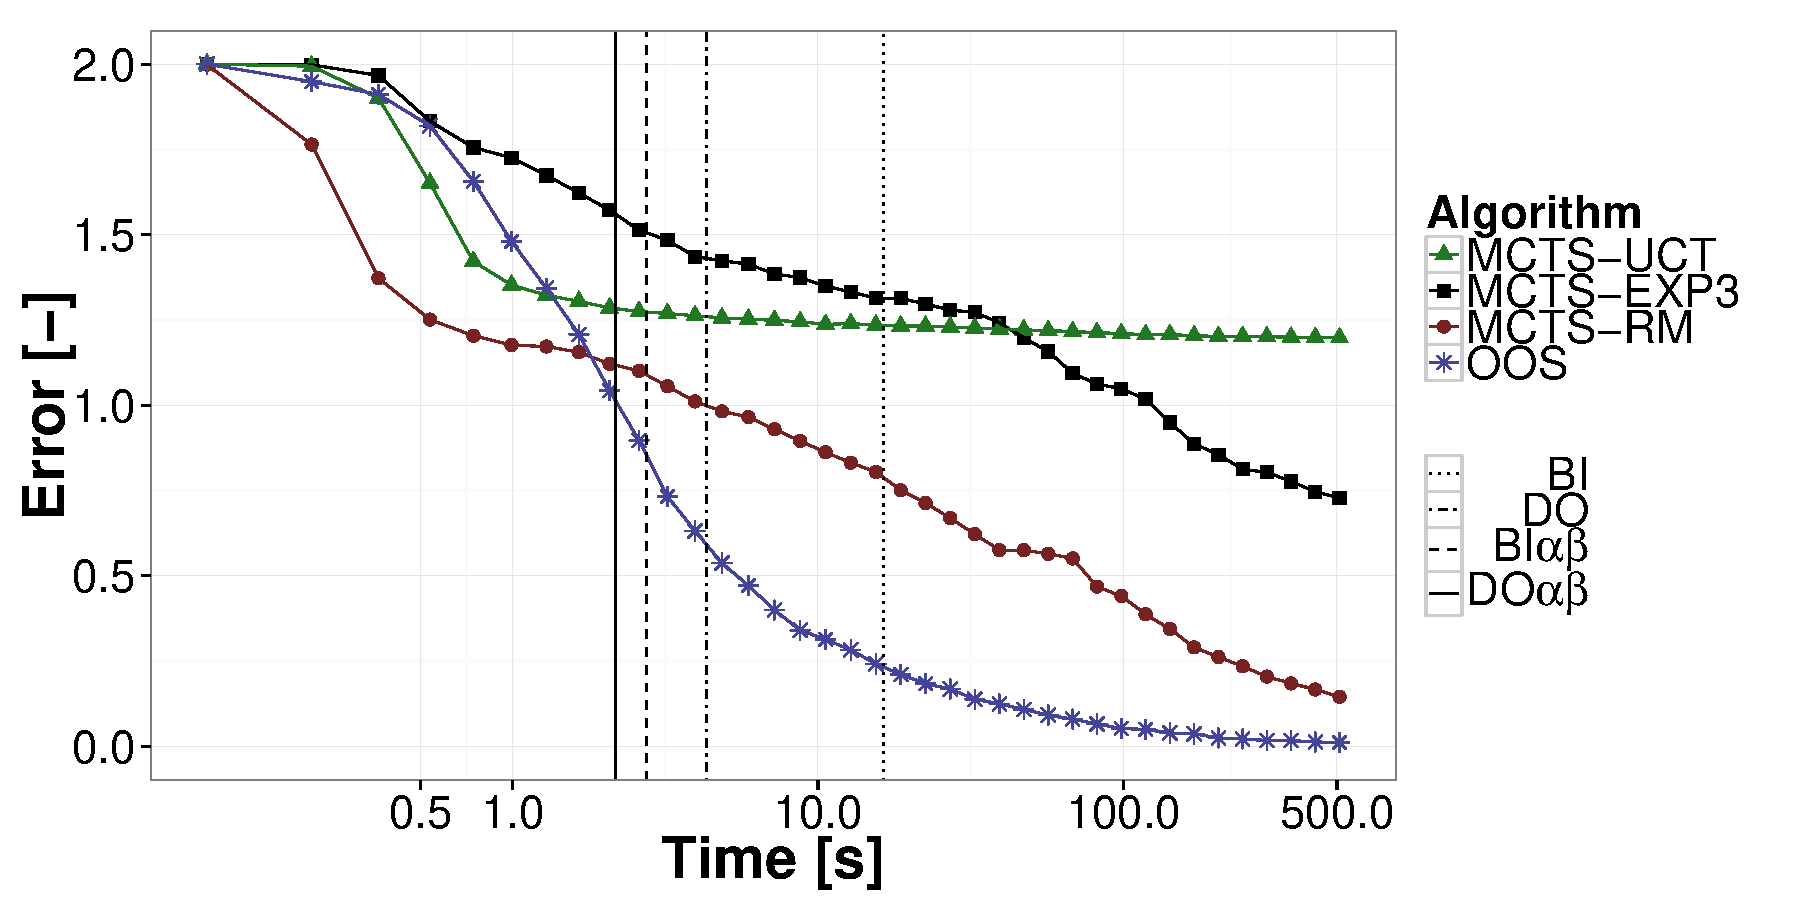
\includegraphics[width=0.85\textwidth]{figures/convergence-peg.pdf}
\caption{Convergence of sampling algorithms on pursuit-evasion game, on $4\times4$ graph, with depth set to $4$. The vertical lines correspond to computation times of exact algorithms.} \label{fig:off:conv:peg}
\end{figure}

We turn to convergence of the sampling algorithms.
In terms of number of iterations per second, again RM was the fastest and OOS the second fastest with similar performance as in Goofspiel.
UCT achieved slightly less ($1.7\times10^5$ iterations per second), and Exp3 only $2.6\times10^4$ iterations.
The results are depicted in Figure~\ref{fig:off:conv:peg} for the smaller $4\times4$ graph and $4$ moves for each player (note again the logarithmic horizontal scale).
The starting positions were selected such that there does not exist a pure NE strategy in the game.
The results again show that OOS is overall the fastest out of all sampling algorithms.
During the first iterations, RM preform similarly, however, OOS is able to keep the convergence rate, RM converges more slowly.
UCT again converges to an exploitable strategy with error $1.16$ at best in the time limit of $500$ seconds ($C=2$).
Finally, Exp3 converges even more slowly compared to Goofspiel.
The main difference between the games is the size of the branching factor for the second player (pursuer controls two simultaneously moving units), which can cause more difficulties for the sampling algorithms to estimate good strategies.

As before, the vertical lines represent times for exact algorithms.
In pursuit-evasion game of this setting, $\doab$ is slightly faster and finishes first in $2.77$ seconds, following by $\biab$ ($2.89$ seconds), \textsc{DO} ($5.48$ seconds), and \textsc{BI} ($12.5$).

\subsubsection{Oshi-Zumo}
\begin{figure}
\centering
	\begin{subfigure}{0.49\textwidth}
		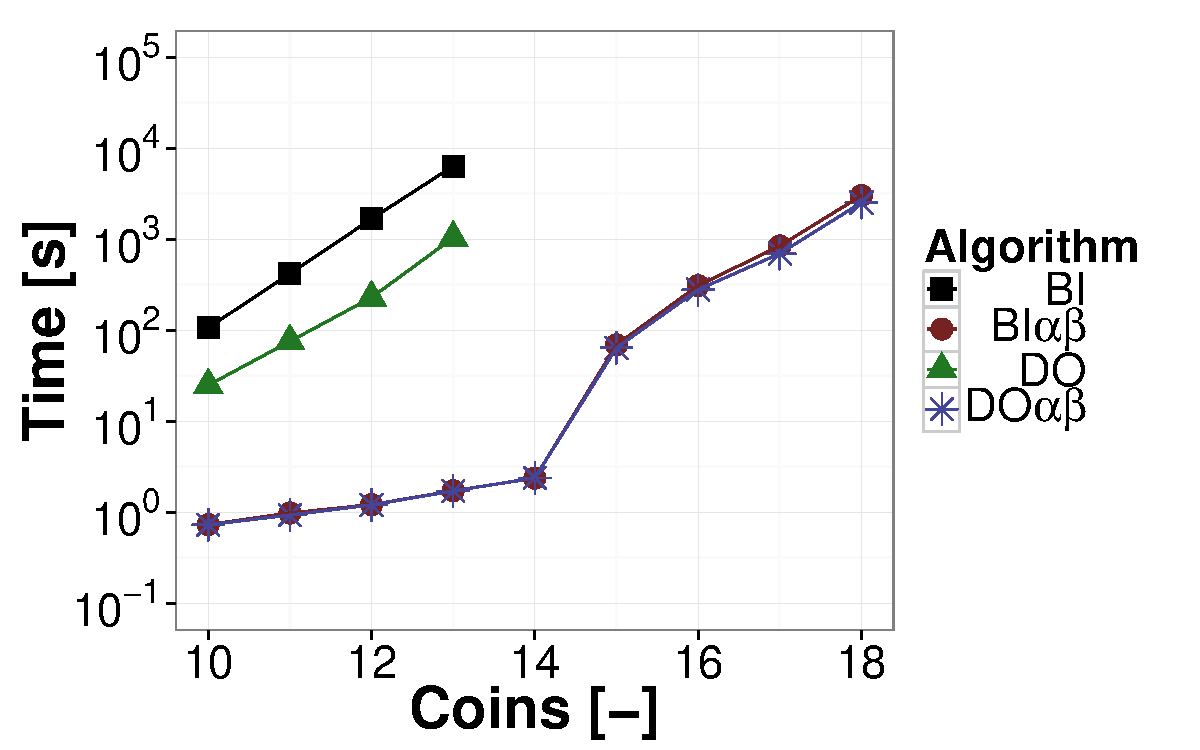
\includegraphics[width=1\textwidth]{figures/OZ-K4.pdf}\caption{}\label{fig:off:res:oz4}
	\end{subfigure}
	\begin{subfigure}{0.49\textwidth}
		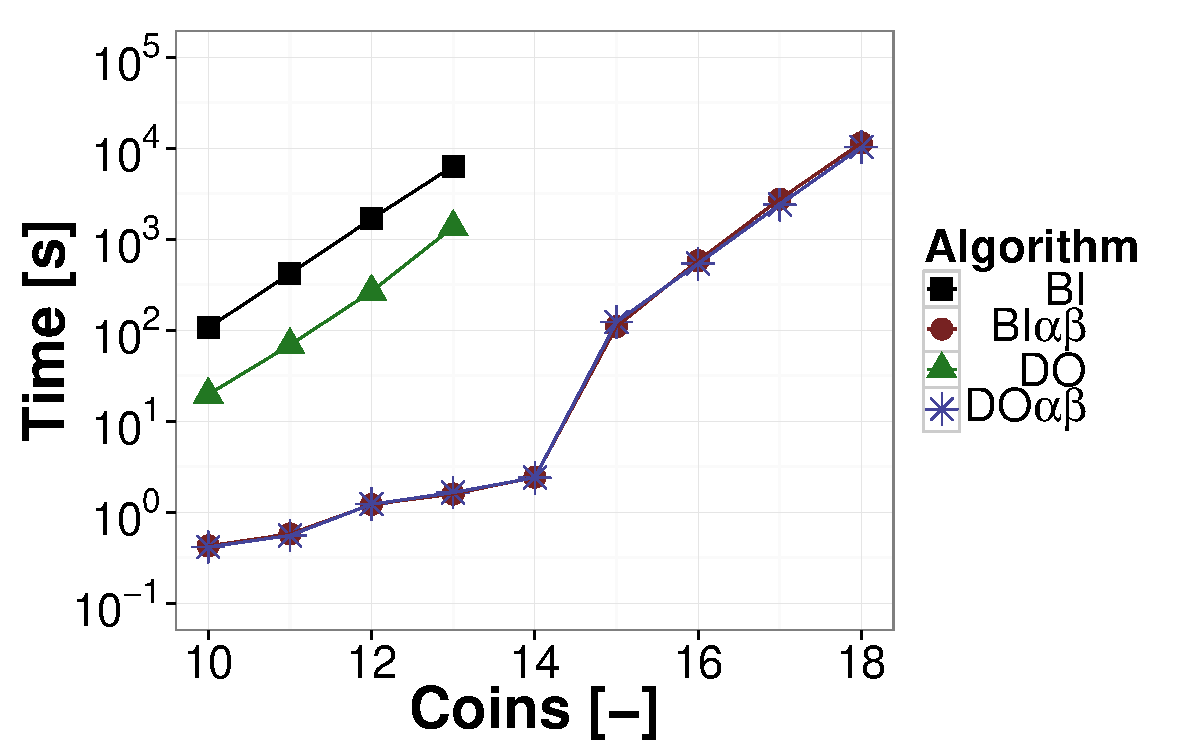
\includegraphics[width=1\textwidth]{figures/OZ-K4-BF.pdf}\caption{}\label{fig:off:res:oz4-bf}
	\end{subfigure}
\caption{Running times of exact algorithms on Oshi-Zumo with $K$ set to $4$ and increasing number of coins: subfigure (a) depicts the results for binary utilities, (b) depicts the results with point utilities.} \label{fig:off:res:oz}
\end{figure}

Many instances of the Oshi-Zumo game have Nash equilibria in pure strategies regardless on the type of utility function.
Although this does not hold for all the instances, the size of the subgames with pure NE are rather large and cause dramatic computation speed-up for both algorithms using serialized alpha-beta search.
If the game does not have equilibria in pure strategies, the mixed strategies are still required only near the root node and large end-games are solved using alpha-beta search.
Note that this is different to pursuit-evasion games, where mixed strategies were necessary close to the end of the game tree.
\reviewchange{
Figure~\ref{fig:off:res:oz} depicts the results with the parameter $K$ set to $4$ and for two different settings of utility function\footnote{\reviewchange{We have also performed the same experiments with $K$ set to $3$, but the conclusions were the same as in case $K=4$.}}; either a win-tie-loose utilities (left subfigure) or point utilities (right subfigure).}
In both cases, the graphs show the breaking point when the game stops having an equilibrium in pure strategies ($15$ coins and more for each player).
The advantage of $\biab$ and $\doab$ algorithms that exploit serialized variants of alpha-beta algorithms is dramatic.
We can see that both \textsc{BI} and \textsc{DO} scale rather badly.
The algorithms were able to scale up to $13$ coins in reasonable time.
For setting with $K=4$ and $13$ coins, it takes almost $2$ hours for \textsc{BI} to solve the game (the algorithm evaluates $1.5\times10^7$ nodes) regardless of the utility values.
\textsc{DO} improves the performance slightly (the algorithm evaluates $2.8\times10^6$ nodes in $17$ minutes \reviewchange{for the win-tie-loose utilities; the performance is slightly worse for point utilities: $5\times10^6$ nodes in $23$ minutes).}
Both $\biab$ and $\doab$, however, solved a single alpha-beta search on each serialization finding a pure NE.
Therefore, their performance is identical and it takes around $1.5$ seconds to solve the game for both types of utilities.
Although with an increasing number of coins the algorithms $\biab$ and $\doab$ need to find mixed Nash equilibria, their performance is very similar for both types of utilities.
\reviewchange{
As expected, the case with point utilities is more challenging and the algorithms scale worse -- for $18$ coins both algorithms solve the game with win-tie-loose utilities in approximately $1$ hour ($\biab$ in $50$ minutes, $\doab$ in $64$), it takes the algorithms around $3$ hours to solve the case with point utilities ($\biab$ in $191$ minutes, $\doab$ in $172$ minutes).
}

\begin{figure}[t]
\centering
	\begin{subfigure}{0.85\textwidth}
		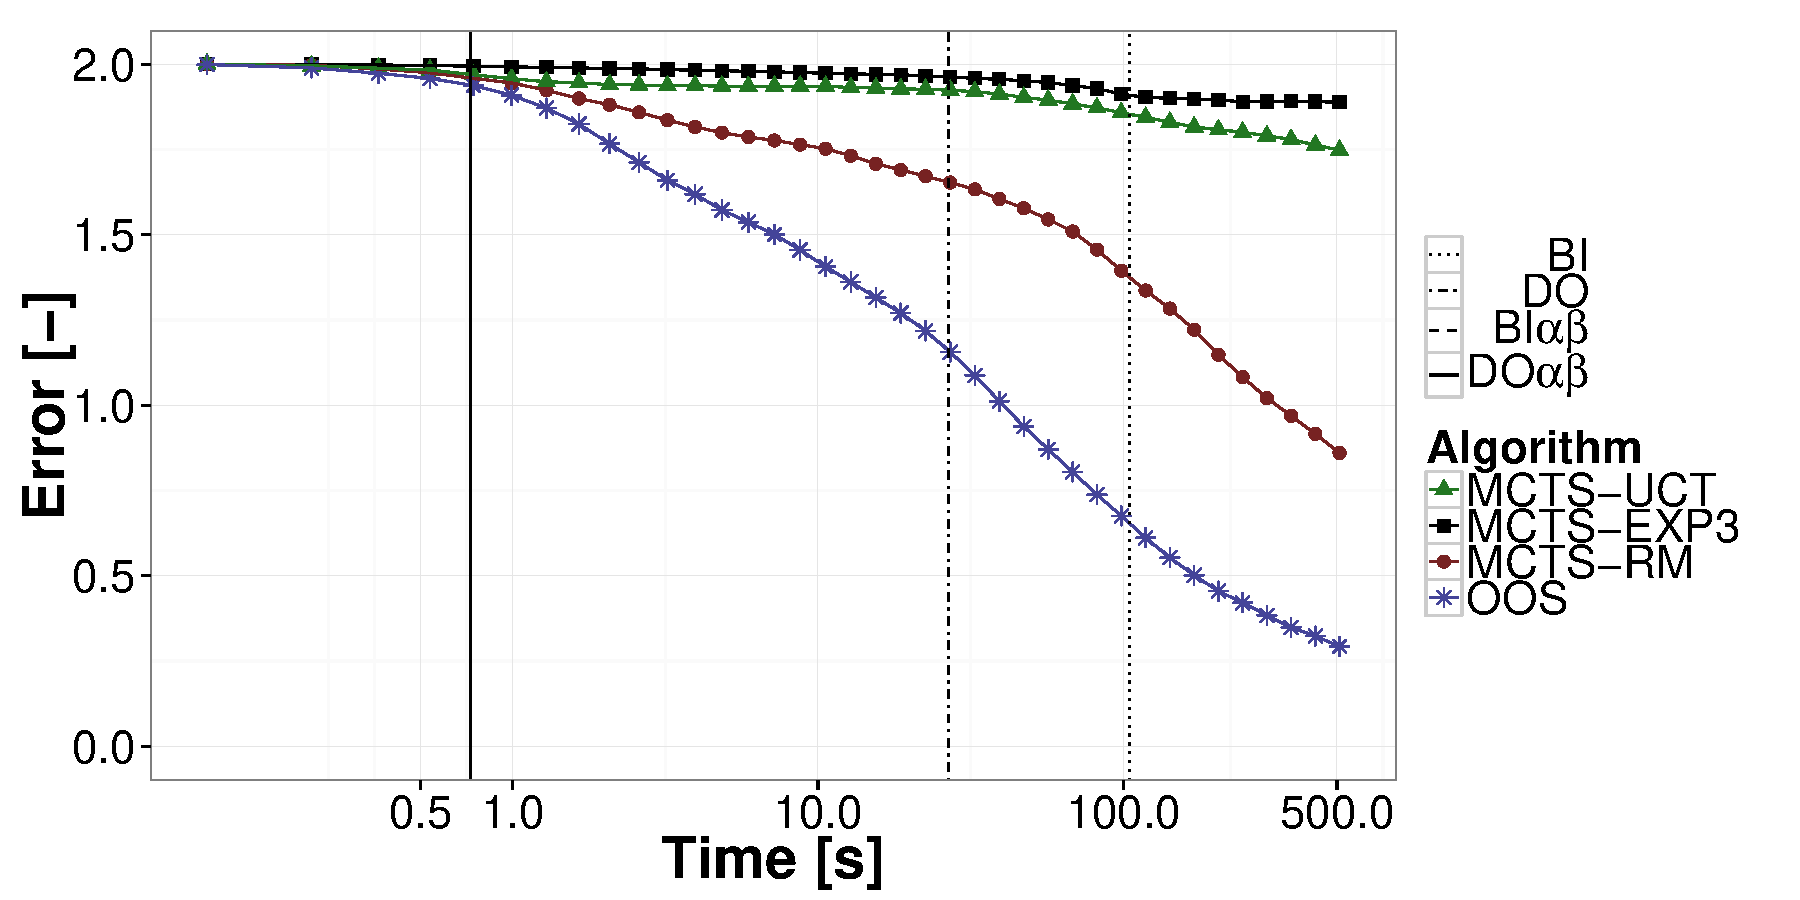
\includegraphics[width=1\textwidth]{figures/convergence-oz.pdf}
	\end{subfigure}
	\begin{subfigure}{0.85\textwidth}
		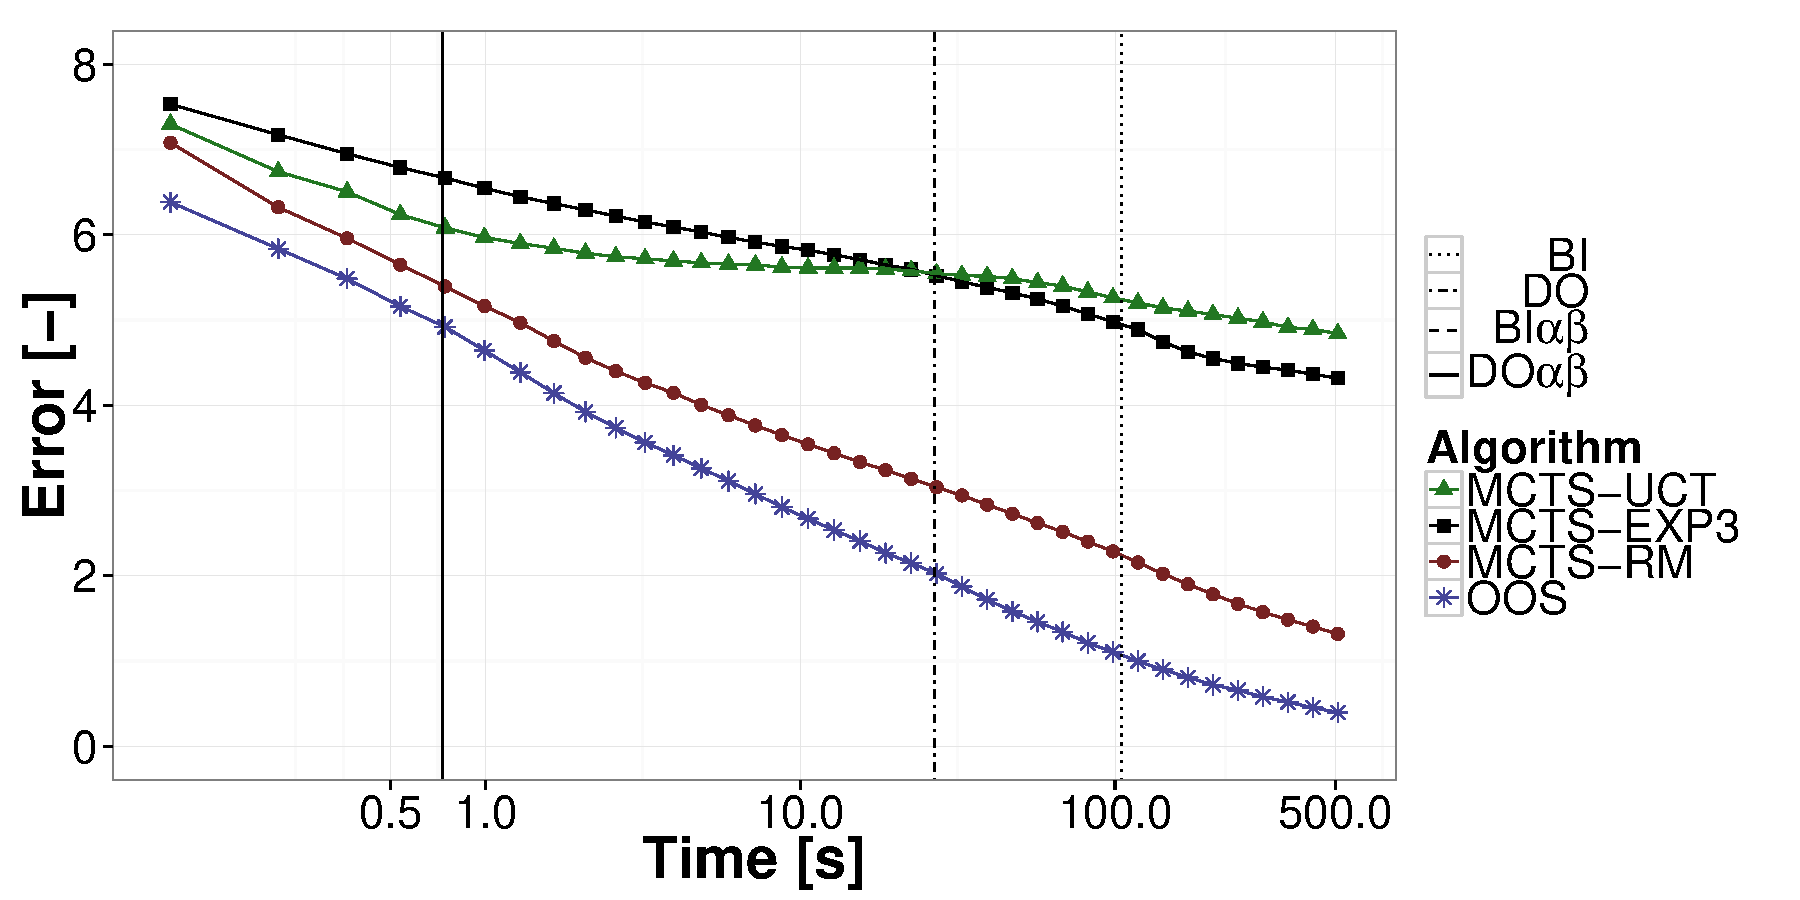
\includegraphics[width=1\textwidth]{figures/convergence-oz-bf.pdf}
	\end{subfigure}
\caption{Convergence of sampling algorithms on Oshi-Zumo game, with $10$ coins, $K=3$, and $M=1$. The vertical lines correspond to computation times of exact algorithms.
(Top) Oshi-Zumo with win-tie-loose utility values;
(Bottom) Oshi-Zumo with point utilities.} \label{fig:off:conv:oz}
\end{figure}

Turning to the sampling algorithms reveals that the game is difficult to approximate even in the win-tie-lose setting.
Figure~\ref{fig:off:conv:oz} depicts results for convergence of the sampling algorithms for the game with $10$ coins, $K$ set to $3$ and minimum bid set to $1$. This is an easy game for $\doab$ and $\biab$ with pure strategy and both of these algorithms are able to solve the game in less than a second ($0.73$). However, due to large branching factor for both players ($10$ actions at the root node for each player) all sampling algorithms converge extremely slowly. The performance of the algorithms in terms of iterations per second is similar to the previous games, however, OOS is slightly better in this case with $1.9\times10^5$ iterations per second compared to the second RM with $1.6\times10^5$ iterations per second.

As before, OOS is the best converging algorithm, however, in a given time limit ($500$ seconds) the reached error was only slightly below $0.3$ ($0.29$). On the other hand, all of the other sampling algorithms perform significantly worse -- RM ends with error slightly over $1$, UCT ($C=2$) with $1.50$, and Exp3 with $1.88$.
This confirms our findings from the previous experiment that increasing branching factor slows down the convergence rate.
Secondly, since there is a pure Nash equilibrium in this particular game configuration, the convergence of the algorithms is also slower since they essentially mix the strategy during the iterations in order to explore the unvisited parts of the game tree. Since none of the sampling algorithms can directly exploit this fact, their performance in offline solving games like Oshi-Zumo is not compelling. On the other hand, the existence of pure NE explains the better performance of UCT compared to Exp3 that is forced to explore more broadly.
\reviewchange{Moreover, convergence takes even more time in the point utility case, since the range of the utility values is larger.
OOS is again the fastest and converges to error $0.45$ within the time limit, RM to $1.41$, UCT ($C=4$) to $3.1$, and Exp3 $3.7$.}


\subsubsection{Random Games}
\begin{figure}[t]
\centering
	\begin{subfigure}{0.49\textwidth}
		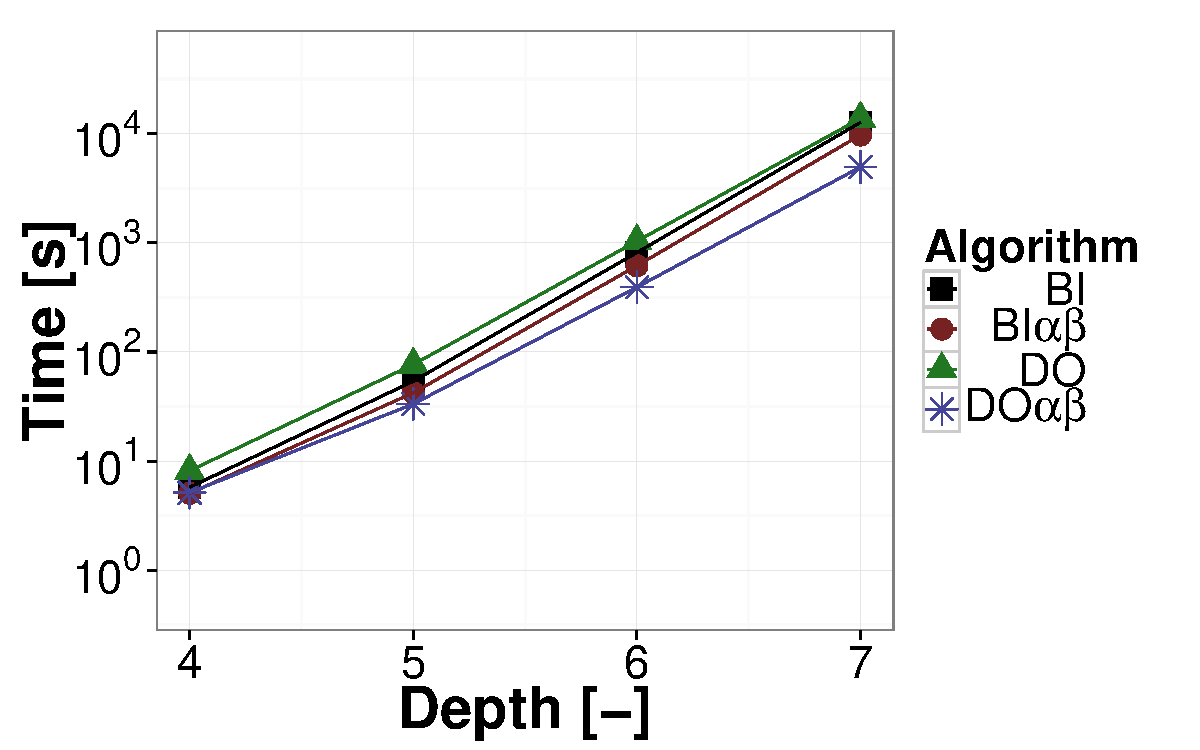
\includegraphics[width=1\textwidth]{figures/RG-BF4-BIN-FALSE.pdf}\caption{}\label{fig:off:res:rgbf4}
	\end{subfigure}
	\begin{subfigure}{0.49\textwidth}
		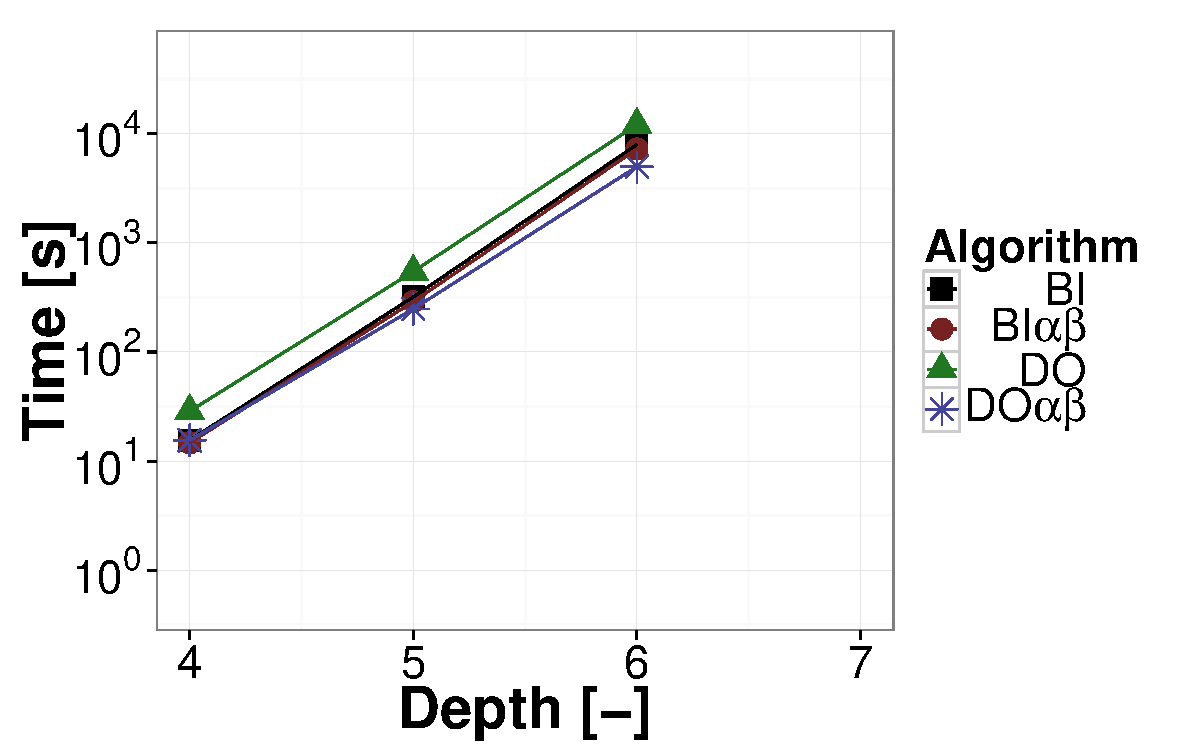
\includegraphics[width=1\textwidth]{figures/RG-BF5-BIN-FALSE.pdf}\caption{}\label{fig:off:res:rgbf5}
	\end{subfigure}
\caption{Running times of exact algorithms on randomly generated games with increasing depth: subfigure (a) depicts the results with branching factor set to $4$ actions for each player, (b) depicts the results with branching factor $5$.} \label{fig:off:res:rg}
\end{figure}

In the first variant of the randomly generated games we used games with utility values randomly drawn from a uniform distribution $[0,1]$.
Such games represent an extreme case, where neither alpha-beta search, nor double-oracle algorithm can save much computation time, since each action can lead to arbitrarily good or bad terminal state.
In these games, \textsc{BI} algorithm is typically the fastest.
Even though both $\biab$ and $\doab$ evaluate marginally less nodes ($\approx90\%$), the overhead of the algorithms (repeated calculation of alpha-beta algorithm, repeatedly solving linear programs, etc.) causes slower runtime performance in this case.

However, completely random games are rarely instances that need to be solved in practice.
The situation changes, when we use the intuition of good and bad moves and thus add correlation to the utility values.
Figure~\ref{fig:off:res:rg} depicts the results for two different branching factors $4$ and $5$ for each player and increasing depth.
The results show that $\doab$ outperforms all remaining algorithms, although the difference is rather small (still statistically significant).
On the other hand, \textsc{DO} without serialized alpha-beta is not able to outperform \textsc{BI}.
This is most likely caused by a larger support in mixed subgame equilibria that cause enumerating most of the actions by the double-oracle algorithm.
Moreover, this is also demonstrated by the performance of $\biab$ that is only slightly better compared to \textsc{BI}.

The fact that serialized alpha-beta is less successful in randomly generated games is noticeable also when comparing the number of evaluated nodes.
For case with branching factor set to $4$ for both players, and depth $7$, \textsc{BI} evaluates almost $1.8\times10^7$ nodes in almost $3.5$ hours, while $\biab$ evaluates more than $\approx1\times10^7$ nodes in almost $3$ hours.
\textsc{DO} evaluates even more nodes compared to $\biab$ ($\approx1.2\times10^7$) and it is slower compared to both \textsc{BI} and $\biab$.
Finally, $\doab$ evaluates $\approx2\times10^6$ nodes on average and it takes the algorithm slightly over $80$ minutes.

\begin{figure}[t]
\centering
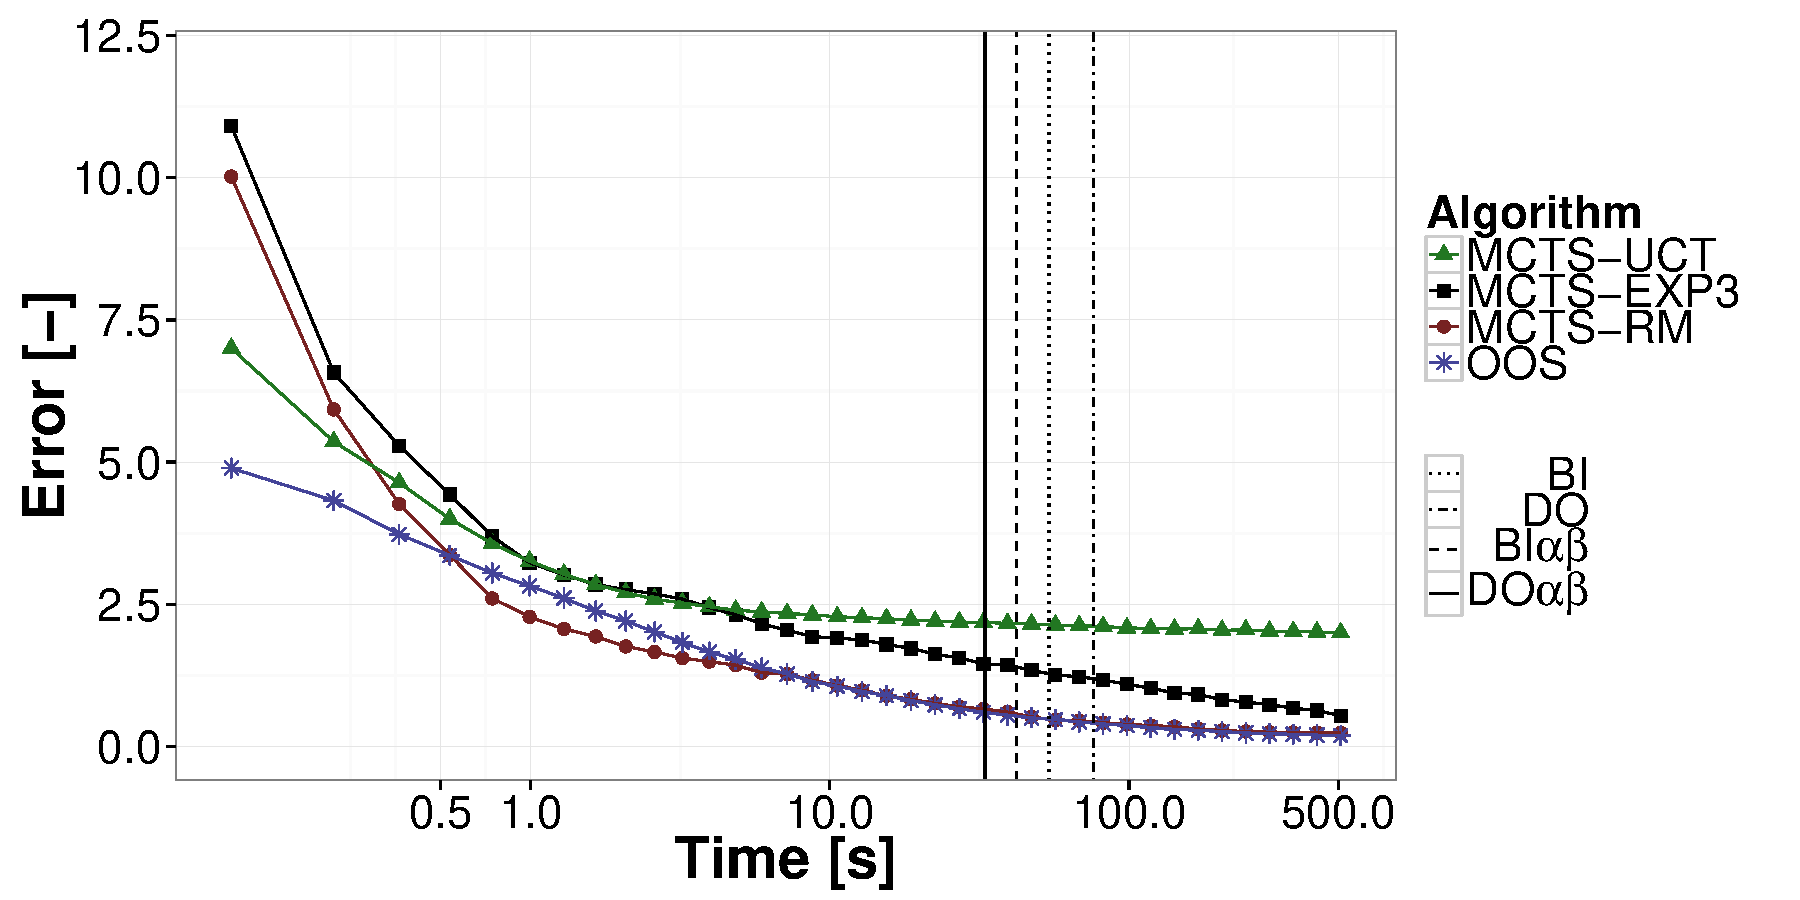
\includegraphics[width=0.85\textwidth]{figures/convergence-rg.pdf}
\caption{Convergence of sampling algorithms on random game with branching factor $4$ and depth $5$. The vertical lines correspond to computation times of exact algorithms.} \label{fig:off:conv:rg}
\end{figure}

Figure~\ref{fig:off:conv:rg} depicts the results for convergence of the sampling algorithms for the random game with correlated utility values, branching factor set to $4$ and depth $5$.
The number of iterations per second is similar to Goofspiel, with Exp3 being the exception able to achieve more than $6.5\times10^4$ iterations per second, which is still significantly the lowest number of iterations.
Interestingly, there is a much less difference between the performance of the sampling algorithms in this game.
Since these games are generally more mixed (\ie NE require to use mixed strategies in many states of the game), they are much more suitable for the sampling algorithms.
OOS can be considered a winner in this setting, however, the performance of RM is very similar.
Again, since the game is more mixed, Exp3 outperforms UCT in the longer run.
Exploration constant for UCT was set to 12 due to larger utility variance in this setting.

\subsubsection{Tron}

\begin{figure}
\centering
	\begin{subfigure}{0.49\textwidth}
		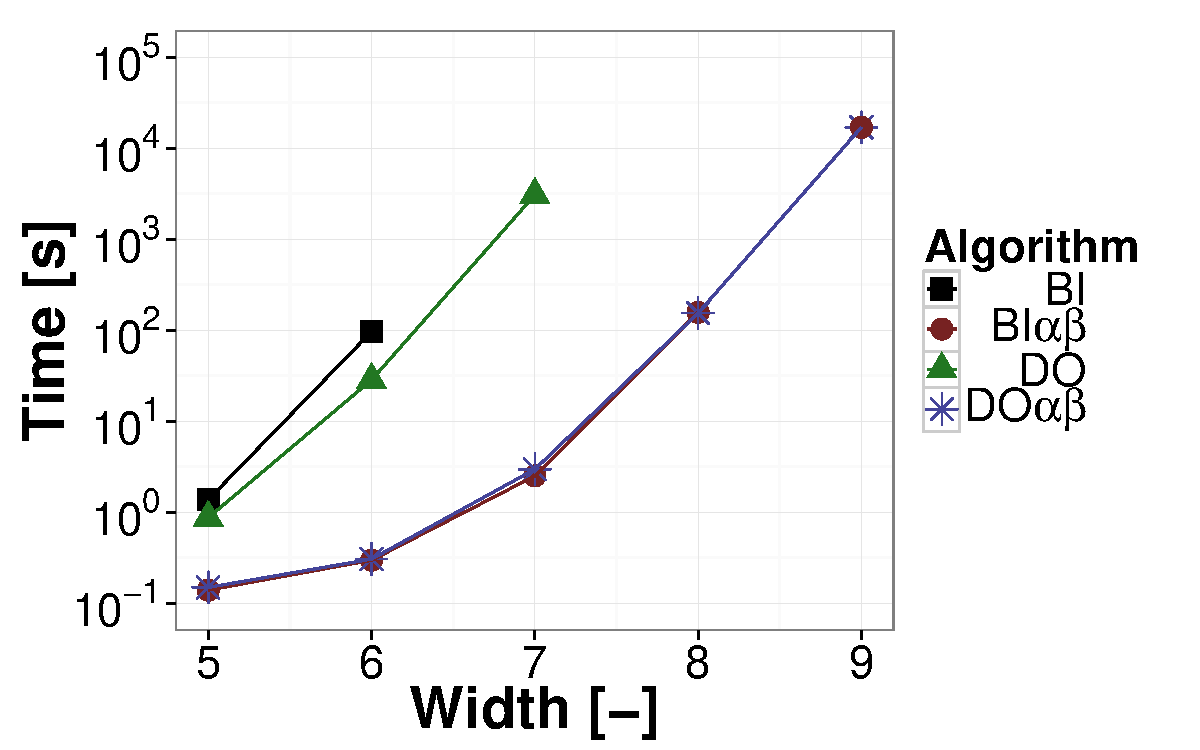
\includegraphics[width=1\textwidth]{figures/Tron-1.pdf}\caption{}\label{fig:off:res:tron1}
	\end{subfigure}
	\begin{subfigure}{0.49\textwidth}
		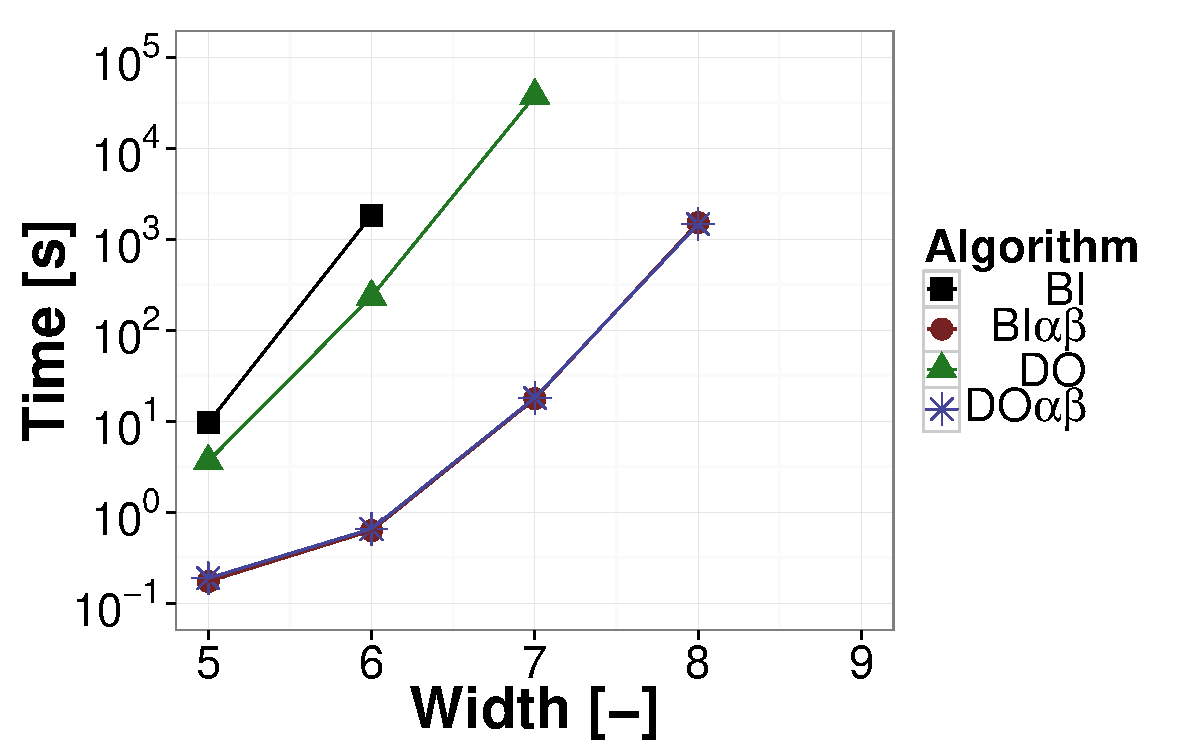
\includegraphics[width=1\textwidth]{figures/Tron-2.pdf}\caption{}\label{fig:off:res:tron2}
	\end{subfigure}
\caption{Running times of exact algorithms on Tron with increasing $width$ of the graph: subfigure (a) depicts the results with $height$ of the graph set to $width - 1$, (b) depicts the results with $height = width$.} \label{fig:off:res:tron}
\end{figure}

Performance of exact algorithms in Tron is affected by the fact that pure NE exist in all smaller instances \reviewchange{
(the results are depicted for two different ratios of dimensions of the grid in Figure~\ref{fig:off:res:tron})}.
Therefore, $\biab$ and $\doab$ are essentially the same since serialized alpha-beta is able to solve the game.
Moreover, since the size of the game increases dramatically with increasing size of the grid (the longest branch of the game tree has $\left(0.5\cdot w\cdot l - 1\right)$ joint actions, where $w$ and $l$ are dimensions of the grid), the performance of standard BI is very poor.
While BI is able to solve the grid $5\times6$ in $96$ seconds, it takes around $30$ minutes to solve $6\times6$ grid.
By comparison, DO solves the $6\times6$ instance in $235$ seconds, and both $\biab$ and $\doab$ in $0.6$ seconds.
\reviewchange{
$\biab$ and $\doab$ scale much better and the largest graph these algorithms solved had size $9\times9$ taking almost $2$ days to solve.
}

\begin{figure}[t]
\centering
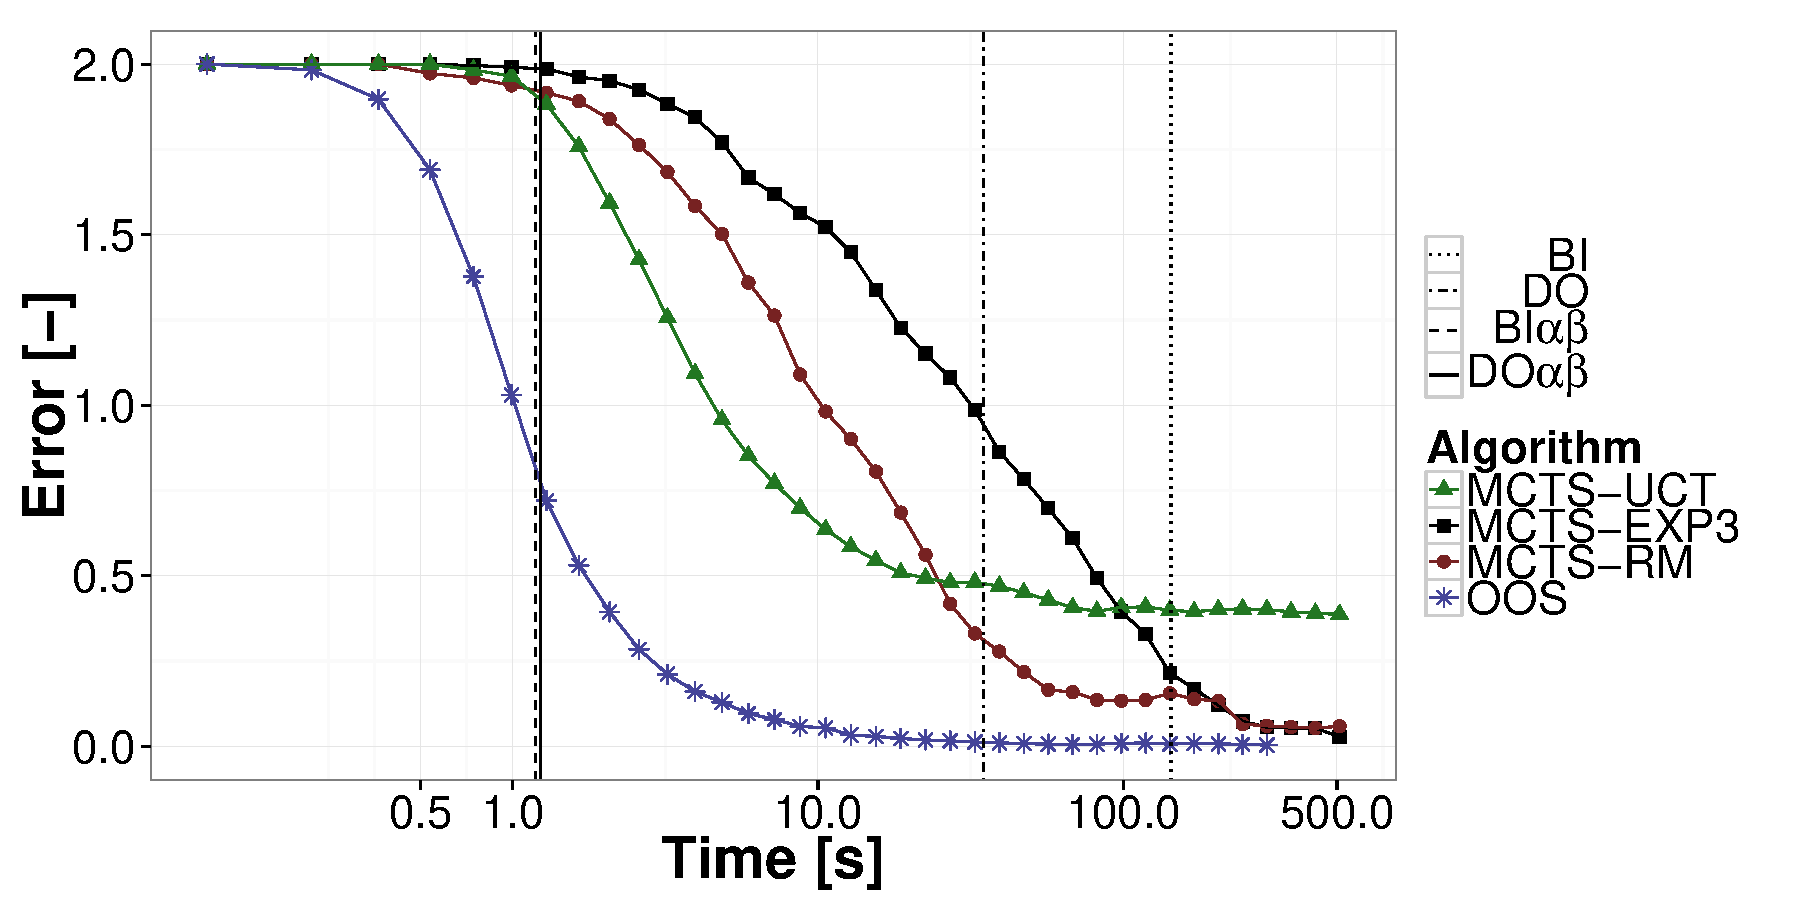
\includegraphics[width=0.85\textwidth]{figures/convergence-tron.pdf}
\caption{Convergence comparison of different sampling algorithms on Tron on grid $5\times6$. The vertical lines correspond to computation times for exact algorithms.} \label{fig:off:conv:tron}
\end{figure}

The size of the game tree in Tron also causes slow convergence for sampling algorithms.
This is apparent also in the number of iterations that is slightly slower for the algorithms.
OOS is the fastest performing $1.3\times 10^5$ iterations per second, RM achieves $1.2\times 10^5$ iterations, UCT only $8\times10^4$, and Exp3 is again the slowest with $7.8\times10^4$ iterations per second.
Figure~\ref{fig:off:conv:tron} depicts the results for the grid $5\times6$.
Consistently with the previous results, OOS performs the best and it is able to converge to very close to exact solution in $300$ seconds.
Similarly, both RM and Exp3 are again eventually able to converge to a very small error, however, it take them more time and in the time limit they achieve error $0.05$, or $0.02$ respectively.
Finally, UCT ($C=5$) performs reasonably good during the first $10$ seconds, where the exploitability is better than both RM and Exp3.
This is most likely due to existence pure NE, however, the length of the game tree prohibits UCT to converge and the best error the algorithm was able to achieve in the time limit was equal to $0.68$.

\subsubsection{Summary of Offline Equilibrium Computation Experiments}

The offline comparison of the algorithms offers several conclusions.
Among the exact algorithms, $\doab$ is clearly the best algorithm, since it typically outperforms all other algorithms (especially in pursuit-evasion games and random games). Although for smaller games (\eg Goofspiel with $5$ cards)  $\biab$ can be slightly faster, this difference is not significant and $\doab$ is never significantly slower compared to $\biab$.

Among the sampling algorithms, OOS is the clear winner since it is often able to quickly converge to a very small error and significantly outperforms all variants of MCTS.
On the other hand, comparing OOS and $\doab$, the exact $\doab$ algorithm is always faster and it is able to find an exact solution much faster compared to OOS.
Moreover, $\doab$ has significantly lower memory requirements since it is a depth-first search algorithm and does not use any form of global cache, while OOS iteratively constructs the game tree in memory.

\subsection{Online Search}

We now compare the performance of the algorithms in head-to-head matches in large instances of the same games as we used in the offline equilibrium computation experiments. Each algorithm has a strictly limited computation time per move set to one or five seconds. After this time, it has to output an action to be played in the current game state and afterwards, it is informed about the action selected by its opponent. The game proceeds to the following state and the algorithms have additional time for computation. As described in Section~\ref{sec:online}, all algorithms keep results of previous computations and do not start form scratch in the following move. Since the results with one and five seconds of computation are practically the same, we presents the results with one second in details and only comment on the five second results later.

We compare all of the approximative sampling algorithms and $\doab$ as a representative of backward induction algorithms, because it was clearly the fastest algorithm in all of the considered games.
Finally, we also included random player (denoted RAND) into the tournament to confirm that the algorithms choose better strategies than the simple random game play.
%In the following experiments, we aim to identify the algorithms that are most suitable in the online search setting and study the relation of the performance in approximating the equilibrium in the offline setting and actual game playing performance in the matches.
We report expected rewards and win rates of the algorithms, in which a tie is counted as half win.
The parameters of the algorithms are tuned for each domain separately.
We first present the comparison of different algorithms and we discuss the influence of the parameters in Subsection~\ref{sec:eval:online:tuning}.

\reviewchange{In this subsection, we show cross tables of each algorithm (on the row) matched up against each competitor algorithm (on the column).}
Each entry represents a mean of at least $1000$ matches with the half of the width of the $95\%$ confidence interval in brackets, \eg $52.9(0.3)$ refers to $52.9\% \pm 0.3\%$.
\reviewchange{The result shown is the win rate for the row player, so as an example in the standard game of Goofspiel (top of Table~\ref{fig:matches:goof}) $\doab$ wins $67.2 \% \pm 1.4 \%$ of games against the random player.}

\subsubsection{Goofspiel}

\begin{table}
\centering
\begin{scriptsize}

Goofspiel: 13 cards, unknown point card sequence, win rate
\begin{tabular}{|r|cccccc|}\hline
&$\doab$&OOS(0.2)&UCT(0.6)&EXP3(0.3)&RM(0.1)&RAND\\\hline
$\doab$&&51.6(3.2)&60.1(3.0)&54.0(3.4)&58.7(4.2)&67.2(1.4)\\
OOS&48.4(3.2)&&51.2(2.1)&52.5(2.2)&47.9(3.0)&81.4(1.7)\\
UCT&39.9(3.0)&48.8(2.1)&&55.6(2.1)&46.6(4.7)&77.3(1.8)\\
EXP3&46.0(3.4)&47.5(2.2)&44.4(2.1)&&41.0(3.0)&86.1(1.5)\\
RM&41.3(4.2)&52.1(3.0)&53.4(4.7)&59.0(3.0)&&84.0(1.1)\\
RAND&32.8(1.4)&18.6(1.7)&22.7(1.8)&13.9(1.5)&16.0(1.1)&\\
\hline
\end{tabular}

Goofspiel: 13 cards, known point card sequence, win rate
\begin{tabular}{|r|cccccc|}\hline
&$\doab$&OOS&UCT&EXP3&RM&RAND\\\hline
$\doab$&&30.8(2.7)&39.3(3.0)&33.8(2.9)&32.7(2.7)&67.2(2.9)\\
OOS&\textbf{69.2(2.7)}&&46.2(3.0)&51.8(3.0)&\textbf{49.6(3.0)}&83.8(2.3)\\
UCT&60.7(3.0)&\textbf{53.8(3.0)}&&\textbf{57.1(2.9)}&48.6(2.9)&79.5(2.5)\\
EXP3&66.2(2.9)&48.2(3.0)&42.9(2.9)&&46.5(3.0)&\textbf{85.8(2.1)}\\
RM&67.3(2.7)&50.4(3.0)&\textbf{51.4(2.9)}&53.5(3.0)&&84.2(2.2)\\
RAND&32.8(2.9)&16.2(2.3)&20.5(2.5)&14.2(2.1)&15.8(2.2)&\\
\hline
\end{tabular}

Goofspiel: 13 cards, known point card sequence, expected reward
\begin{tabular}{|r|cccccc|}\hline
&$\doab$&OOS(0.3)&UCT(0.8)&EXP3(0.2)&RM(0.1)&RAND\\\hline
$\doab$&&-7.59(0.97)&-1.80(0.91)&-7.30(0.87)&-5.89(1.01)&6.67(0.99)\\
OOS&7.59(0.97)&&1.19(0.78)&0.30(0.78)&0.35(0.76)&14.42(0.96)\\
UCT&1.80(0.91)&-1.19(0.78)&&-0.77(0.76)&-1.94(0.73)&13.30(1.00)\\
EXP3&7.30(0.87)&-0.30(0.78)&0.77(0.76)&&-1.65(0.72)&15.89(1.00)\\
RM&5.89(1.01)&-0.35(0.76)&1.94(0.73)&1.65(0.72)&&14.20(0.98)\\
RAND&-6.67(0.99)&-14.42(0.96)&-13.30(1.00)&-15.89(1.00)&-14.20(0.98)&\\
\hline
\end{tabular}
\end{scriptsize}
\caption{Results of head-to-head matches in Goofspiel variants with exploration parameter settings indicated in the header.}\label{fig:matches:goof}
\end{table}

In head-to-head comparison, we use the standard Goofspiel with 13 cards. Additionally, for the sake of consistency with the offline results, we also evaluate the variant with a fixed known sequence of the point cards, removing all chance nodes. The full game has more than $2.4\times 10^{29}$ leaf nodes and the variant with fixed point card sequence has still more than $3.8\times 10^{19}$ leaf nodes. The results are presented in Table~\ref{fig:matches:goof}, where the top table shows the win rates of the algorithms in the full game and the other two tables the win rates and expected number of points gained by the algorithms in the game with a fixed point card sequence. The results for the know card sequence are the mean of $10$ fixed random orderings. For each table, the algorithms were set up to optimize the presented measure (\ie win rate or expected points) and the exploration parameters were tuned to the values presented in the header of the table.

First, we can see that finding a good strategy in Goofspiel is difficult for all the algorithms.
This is noticeable thanks to the results of RAND player, that performs reasonably well
(RAND typically loses almost every match in all the remaining game domains).
Next, we analyze the results of the $\doab$ algorithms compared to the sampling algorithms.
The larger game variant seems to be too large and noisy for the sampling algorithms to converge to good strategies.
$\doab$ with a domain-specific heuristic evaluation function outperforms all sampling algorithms.
With the exception of OOS, the performance difference is statistically significant.
In the game variants with the fixed point card sequence, the situation is the opposite.
$\doab$ does not win significantly against any of the sampling algorithms.
The sampling algorithms can already find better state evaluations than the hand-coded heuristic evaluation function in $\doab$.
Also, the limited overhead due to short and fixed length of this game could favor sampling methods compared to the
matrix constructions in $\doab$.

The differences in the performance of sampling algorithms are relatively small.
In the variant with unknown card sequence, Exp3 performs worst, outperforming only the random player.
OOS significantly outperforms only Exp3 and RM is the best among the sampling algorithms, winning over all other algorithms and with the exception of OOS significantly.
In the game with fixed card sequence, RM still wins most matches against any of the opponents, but UCT manages to better exploit the weaker opponents and win more often than RM against EXP3 and OOS.
When optimizing the expected points OOS wins slightly against all sampling algorithms, but with the exception of UCT, it is not statistically significant. RM looses against OOS slightly, wins significantly against UCT and EXP3.

In summary, RM is the only algorithm that did not loose significantly against any other sampling algorithm in any other game variant and often won significantly. Exp3 was weakest overall and the performance of UCT was very unstable along game variants and various opponents.

\vlisy{stress in conclusions that RM is most stable in choice of the parameter, which is an important advantage}

\subsubsection{Oshi-Zumo}

\begin{table}[t!]
\centering
\begin{scriptsize}

Oshi Zumo: 50 coins, 2$\cdot$3 + 1 positions, win rate
\begin{tabular}{|r|cccccc|}\hline
&$\doab$&OOS(0.2)&UCT(0.4)&EXP3(0.8)&RM(0.1)&RAND\\\hline
$\doab$&&\textbf{79.5(1.7)}&\textbf{76.8(2.6)}&74.0(2.7)&\textbf{81.0(2.4)}&98.8(0.5)\\
OOS&20.5(1.7)&&27.7(2.6)&57.1(2.1)&51.2(2.1)&98.9(0.4)\\
UCT&23.1(2.6)&72.3(2.6)&&\textbf{83.0(2.0)}&70.3(2.6)&\textbf{99.9(0.2)}\\
EXP3&\textbf{26.1(2.7)}&42.9(2.1)&17.0(2.0)&&44.5(2.8)&98.5(0.5)\\
RM&18.9(2.4)&48.8(2.1)&29.6(2.6)&55.5(2.8)&&99.0(0.4)\\
RAND&1.2(0.5)&1.1(0.4)&0.1(0.2)&1.5(0.5)&1.0(0.4)&\\
\hline
\end{tabular}

Oshi Zumo: 50 coins, 2$\cdot$3 + 1 positions, expected reward
\begin{tabular}{|r|cccccc|}\hline
&$\doab$&OOS(0.2)&UCT(0.4)&EXP3(0.8)&RM(0.1)&RAND\\\hline
$\doab$&&\textbf{2.51(0.18)}&\textbf{1.84(0.21)}&\textbf{1.08(0.22)}&\textbf{2.75(0.17)}&3.65(0.09)\\
OOS&-2.51(0.18)&&-0.53(0.19)&-0.57(0.16)&0.25(0.20)&3.87(0.05)\\
UCT&-1.84(0.21)&0.53(0.19)&&0.19(0.15)&0.58(0.17)&\textbf{3.93(0.02)}\\
EXP3&\textbf{-1.08(0.22)}&0.57(0.16)&-0.19(0.15)&&0.53(0.16)&3.86(0.04)\\
RM&-2.75(0.17)&-0.25(0.20)&-0.58(0.17)&-0.53(0.16)&&3.87(0.04)\\
RAND&-3.65(0.09)&-3.87(0.05)&-3.93(0.02)&-3.86(0.04)&-3.87(0.04)&\\
\hline
\end{tabular}

Oshi Zumo: 50 coins, 2$\cdot$3 + 1 positions, win rate, evaluation function
\begin{tabular}{|r|cccccc|}\hline
&$\doab$&OOS(0.3)&UCT(0.8)&EXP3(0.8)&RM(0.1)&RAND\\\hline
$\doab$&&61.8(3.0)&8.3(1.5)&48.6(3.1)&58.6(3.1)&98.8(0.7)\\
OOS&38.2(3.0)&&23.1(2.6)&33.6(2.9)&44.1(3.0)&99.6(0.4)\\
UCT&\textbf{89.5(1.8)}&\textbf{73.6(2.7)}&&\textbf{83.2(2.3)}&\textbf{70.5(2.8)}&\textbf{99.8(0.3)}\\
EXP3&48.5(3.1)&66.7(2.9)&22.3(2.5)&&57.9(3.0)&98.7(0.7)\\
RM&37.8(3.0)&56.9(3.0)&\textbf{28.4(2.8)}&40.5(2.9)&&99.4(0.5)\\
RAND&1.5(0.8)&0.4(0.4)&0.2(0.2)&1.3(0.7)&0.2(0.3)&\\
\hline
\end{tabular}
\end{scriptsize}
\caption{Results of head-to-head matches in Oshi-Zumo variants with exploration parameter settings indicated in the header. In the first two tables only $\doab$ uses evaluation function and in the third table all algorithms use the evaluation function.}\label{fig:matches:oz}
\end{table}

In Oshi-Zumo, we use the setting with 50 coins, K=3 fields on each side of the board and minimal bet of 1.
%We chose this parameters to be consistent with \cite{XXX}\bbosansky{Missing reference} and to have a game with larger branching factor.
The size of the game is large with strictly more than $10^{15}$ leaves (number of choices of a single player in the game; hence, square of this number is the upper bound on the number of leaves) and 50 actions for each player in the root.

In this game, the evaluation function used by $\doab$ is much stronger than in Goofspiel and all the sampling algorithms without domain specific knowledge perform poorly against this algorithm (see Table~\ref{fig:matches:oz}). The loss is even higher with 5 seconds per move. None of the sampling algorithms perform significantly better than the others.

In the offline experiment (Figure~\ref{fig:off:conv:oz}), none of the sampling algorithms was able to converge anywhere close to the equilibrium in short time. Moreover, the game used in the offline experiments was many orders of magnitude smaller (there were $10$ coins for each player).
In spite of the negative results in the offline experiments, all sampling algorithms are able to find reasonably good strategy.
UCT is clearly the strongest sampling algorithm in all variants.
In win rate, its strongest opponent among the sampling algorithms is RM (UCT wins only 70.3\% of games). Exp3 is the weakest algorithm in optimizing the win rate, but it looses only to UCT in optimizing expected reward. RM is the weakest in that setting.

Because of high quality of the evaluation function in this game, we performed experiments where the rollout simulation was replaced with the evaluation function.
The the results are presented in the third table of Table~\ref{fig:matches:oz}).
The quality of play of all sampling algorithms is significantly improved when using the evaluation function.
However, $\doab$ still wins over OOS and RM in both time settings.
UCT is clearly the best and OOS the weakest.

The reason why UCT performs well in this game is that the game mostly requires pure strategies, rather then precise mixing between multiple strategies (see Section~\ref{sec:eval:domains}). UCT is able to quickly disregard other actions, if a single action is optimal.

\subsubsection{Random Games}

\begin{table}
\centering
\begin{scriptsize}

\begin{tabular}{|r|cccccc|}\hline
&$\doab$&OOS(0.1)&UCT(1.5)&EXP3(0.6)&RM(0.3)&RAND\\\hline
$\doab$&&55.4(3.3)&43.7(2.8)&49.2(2.8)&48.1(2.8)&88.8(1.8)\\
OOS&45.6(3.3)&&33.5(2.5)&43.5(2.7)&42.5(2.8)&85.0(2.4)\\
UCT&\textbf{56.3(2.8)}&\textbf{66.5(2.5)}&&\textbf{67.4(2.5)}&\textbf{55.7(2.6)}&95.9(1.2)\\
EXP3&50.8(2.8)&56.5(2.7)&32.6(2.5)&&42.9(2.7)&\textbf{96.0(1.1)}\\
RM&51.9(2.8)&57.5(2.8)&\textbf{44.3(2.6)}&57.1(2.7)&&93.1(1.5)\\
RAND&11.2(1.8)&15.0(2.4)&4.1(1.2)&4.0(1.1)&6.9(1.5)&\\
\hline
\end{tabular}


\end{scriptsize}
\caption{Win-rate in head-to-head matches of Random games (15,5).}\label{fig:matches:rand}
\end{table}


The next set of matches was played on 10 different random games with each player having 5 actions in each stage and depth 15. Hence, the game has more than $9.3\times 10^{20}$ leaf nodes. In order to compute the win-rates as in other games, we use signum of the utility value defined in Subsection~\ref{sec:eval:domains}. The results are presented in Table~\ref{fig:matches:rand}.

The clearly best performing algorithm in this domain is UCT.
RM is the second, losing only to UCT.
OOS has the weakest performance in spite of good convergence results in the offline settings (see~Figure~\ref{fig:off:conv:rg}).
\reviewchange{
The reason is the quickly growing variance and decreasing number of samples in longer games, which we discuss in more detail in Section~\ref{sec:oos_vs_rm}.
}
%We also performed an experiment with larger branching factor (15) and smaller depth (5), but the results were very similar to this setting.\vlisy{I assume the new OOS would perform much better there!}

\subsubsection{Tron}

\begin{table}[t!]
\centering
\begin{scriptsize}
Tron: 13x13 grid, win rate
\begin{tabular}{|r|cccccc|}\hline
&$\doab$&OOS(0.1)&UCT(0.6)&EXP3(0.5)&RM(0.1)&RAND\\\hline
$\doab$&&\textbf{79.3(2.0})&\textbf{55.6(2.0)}&\textbf{66.7(2.3)}&\textbf{62.6(2.2)}&\textbf{98.6(0.5)}\\
OOS&20.7(2.0)&&29.4(2.2)&46.1(1.8)&38.0(2.2)&97.2(0.5)\\
UCT&44.4(2.0)&70.6(2.2)&&64.8(2.2)&57.0(2.1)&98.0(0.6)\\
EXP3&33.3(2.3)&53.9(1.8)&35.1(2.2)&&44.3(2.3)&97.7(0.5)\\
RM&37.4(2.2)&62.0(2.2)&43.0(2.1)&55.7(2.3)&&97.7(0.7)\\
RAND&1.4(0.5)&2.9(0.5)&2.0(0.6)&2.3(0.5)&2.3(0.7)&\\
\hline
\end{tabular}

Tron: 13x13 grid, win rate, evaluation function
\begin{tabular}{|r|cccccc|}\hline
&$\doab$&OOS(0.1)&UCT(2)&EXP3(0.1)&RM(0.2)&RAND\\\hline
$\doab$&&\textbf{51.5(2.0)}&45.6(1.8)&\textbf{58.0(2.0)}&48.9(2.1)&98.9(0.5)\\
OOS&49.4(1.6)&&52.6(1.3)&54.4(1.2)&\textbf{53.1(1.2)}&97.8(0.7)\\
UCT&\textbf{65.3(2.1)}&46.5(1.3)&&49.8(0.7)&46.5(0.9)&\textbf{99.0(0.4)}\\
EXP3&46.6(2.1)&45.2(1.2)&50.4(0.7)&&45.5(1.0)&98.2(0.6)\\
RM&56.7(2.2)&48.5(1.2)&\textbf{53.2(0.9})&53.9(0.9)&&98.8(0.5)\\
RAND&2.3(0.7)&2.0(0.6)&1.5(0.6)&1.9(0.6)&1.7(0.6)&\\
\hline
\end{tabular}
\end{scriptsize}
\caption{Win-rate in head-to-head matches of Tron with random simulations (top) and evaluation function in the sampling algorithms (bottom).}\label{fig:matches:tron}
\end{table}

The large variant of Tron in our evaluation was played on en empty $13\times 13$ board. The branching factor of this game is up to 4 for each player and its depth is up to 83 moves. This variant of Tron has more than $10^{21}$ leaves in the game tree\footnote{The number only estimates the number of possible paths when both players stay on their half of the board.}.
The results are shown in Table~\ref{fig:matches:tron}.

The evaluation function in Tron quite well approximates the actual situation in the game; hence, $\doab$ strongly outperforms all other algorithms when they do not use the evaluation function (top). Its win-rates are even higher with more time per move.
UCT is its strongest opponent, which loses 55.6\% matches and wins over all other sampling algorithms in mutual matches. This is again because of the low need for mixed strategies in this game.
OOS performs the worst because of the high length of the game. It won only 20.7\% matches against $\doab$ and 29.4\% matches against UCT.
\reviewchange{This is consistent with previous analyses in Tron where the best-performing algorithms, including the winner of the 2011 Google AI Challenge,
were based on depth-limited minimax searches~\cite{DenTeuling12Tron,Perick12Comparison}.}

As in the case of Oshi Zumo, we also run the matches with the evaluation function to replace the random rollout simulation in the sampling algorithms.
The usage of the evaluation function improves the performance of all sampling algorithms.
The difference is most notable for OOS, since using the evaluation function strongly reduces the length of the game.
When sampling algorithms use the evaluation function, $\doab$ is already outperformed by UCT and RM.
Exp3 is the weakest algorithm, but the results among the sampling algorithms are not transitive.
OOS significantly outperforms RM, RM outperforms UCT, UCT outperforms $\doab$, and $\doab$ outperforms OOS. This means that none of the algorithms plays close to the equilibrium and each can be exploited by a well chosen opponent.

\subsubsection{Pursuit-Evasion Game}

\begin{table}
\centering
\begin{scriptsize}

\begin{tabular}{|r|cccccc|}\hline
&$\doab$&OOS(0.3)&UCT(0.8)&EXP3(0.5)&RM(0.1)&RAND\\\hline
$\doab$& \textbf{80.9(2.4)}& 91.3(1.7)& \textbf{63.2(3.0)}& 86.3(2.1)& 78.4(2.6)& 99.9(0.2)\\
OOS(0.2)& 76.3(2.6)& 91.2(1.8)& 57.8(3.1)& 85.8(2.2)& 79.3(2.5)& 99.8(0.3)\\
UCT(1.5)& 75.1(2.7)& \textbf{94.2(1.4)}& 57.6(3.1)& \textbf{88.9(1.9)}& \textbf{82.2(2.4)}& \textbf{100.0(0.0)}\\
EXP3(0.2)& 69.1(2.9)& 92.1(1.7)& 53.1(3.1)& 83.9(2.3)& 75.1(2.7)& 99.8(0.3)\\
RM(0.1)& 81.0(2.4)& 92.7(1.6)& 58.5(3.1)& 86.7(2.1)& 78.6(2.5)& 99.8(0.3)\\
RAND& 4.6(1.3)& 28.8(2.8)& 5.8(1.4)& 1.7(0.8)& 3.1(1.1)& 71.1(2.8)\\
\hline
\end{tabular}

\end{scriptsize}
\caption{Win-rate in head-to-head matches of Pursuit evasion game with time limit of 15 moves and $10\times 10$ grid board.}\label{fig:matches:peg}
\end{table}


Finally, we compared algorithms on the pursuit-evasion game on an empty $10\times 10$ grid with $15$ moves time limit and 10 different randomly selected initial positions of the units. The branching factor is up to 12, causing the number of leaf nodes to be less than $10^{16}$.

The results in Table~\ref{fig:matches:peg} show that the game is strongly biased towards the first player, which is the evader. The self-play results on the diagonal shows that $\doab$ won over 80.9\% matches against itself as the evader. Adding more computational time typically improved the play of the pursuer in self-play. This is caused by more complex optimal strategy of the pursuer. This optimal strategy is more difficult to find due to a larger branching factor (recall that pursuer controls two units) and requirement for more precise execution of strategies (a single move played incorrectly can cause an escape of the evader and can result in losing the game due to the time limit).

Let's first look at the differences in the performance of the algorithms on the side of the pursuer, which are more consistent. We need to compare the different columns, in which the pursuer ties the minimize the values.
The clear winner is UCT, which generally captured the evaders in approximately 40\% of the matches.
The second best pursuer is $\doab$ and the weakest is OOS, which captured the non-random opponent in less than 10\% cases.

The situation is less clear for the evader. Different algorithms performed best agains different opponents.
UCT was best against OOS, Exp3 and RM, but $\doab$ was the best against UCT and itself.
Exp3 is the weakest evader.

\subsubsection{Parameter tuning}\label{sec:eval:online:tuning}

\begin{table}
\centering
\begin{scriptsize}

Goofspiel: 13 cards, unknown point card sequence
\begin{tabular}{|lr|ccccc|c|}\hline
&&$\doab$&OOS(0.6)&UCT(2)&EXP3(0.2)&RM(0.1)&Mean\\\hline
OOS&0.5&49.4(3.2)&50.2(3.0)&54.4(4.2)&54.9(3.0)&49.4(3.0)&51.66\\
OOS&0.4&49.2(3.2)&50.5(3.0)&56.4(4.2)&54.1(3.0)&47.5(3.0)&51.54\\
OOS&0.3&48.2(3.2)&47.6(3.0)&58.4(4.2)&54.3(3.0)&48.0(3.1)&51.3\\
OOS&\textbf{0.2}&48.4(3.2)&50.2(3.0)&58.7(4.2)&54.3(3.0)&47.9(3.0)&\textbf{51.9}\\
OOS&0.1&51.0(3.2)&47.4(3.1)&53.4(4.3)&48.6(3.0)&43.9(3.0)&48.86\\
UCT&1.5&40.7(3.0)&45.4(3.0)&52.4(3.2)&53.9(3.9)&39.4(4.6)&46.36\\
UCT&1&39.6(3.0)&49.9(3.0)&58.3(3.2)&56.1(3.8)&43.1(4.6)&49.4\\
UCT&0.8&36.6(2.9)&51.1(3.0)&60.8(3.2)&59.7(3.8)&46.8(4.7)&51\\
UCT&\textbf{0.6}&39.9(3.0)&53.9(3.0)&61.2(3.1)&62.3(3.8)&46.6(4.7)&\textbf{52.78}\\
UCT&0.4&39.0(3.0)&54.9(3.0)&61.6(3.1)&58.6(3.8)&49.5(4.8)&52.72\\
EXP3&0.5&47.9(3.4)&42.6(3.0)&44.4(3.0)&47.4(3.0)&40.1(3.0)&44.48\\
EXP3&0.4&48.4(3.4)&44.8(3.0)&48.4(3.0)&49.5(3.0)&39.5(3.0)&46.12\\
EXP3&\textbf{0.3}&46.0(3.4)&44.5(3.0)&51.8(3.0)&51.1(3.0)&41.0(3.0)&\textbf{46.88}\\
EXP3&0.2&40.5(3.4)&47.2(3.0)&47.6(3.0)&50.0(3.0)&41.3(3.0)&45.32\\
EXP3&0.1&42.3(3.4)&44.9(3.0)&48.9(3.0)&51.2(3.0)&40.9(3.0)&45.64\\
RM&0.5&42.2(4.2)&44.9(3.0)&43.9(3.0)&46.9(3.0)&42.4(3.0)&44.06\\
RM&0.3&42.6(4.3)&49.3(3.0)&57.9(2.9)&53.9(3.0)&48.5(3.0)&50.44\\
RM&0.2&38.9(3.8)&50.7(3.0)&63.8(2.9)&57.8(3.0)&48.2(3.0)&51.88\\
RM&\textbf{0.1}&41.3(4.2)&54.1(3.0)&61.2(2.9)&58.1(3.0)&51.2(3.0)&\textbf{53.18}\\
RM&0.05&43.0(4.3)&51.6(3.0)&60.1(2.9)&59.0(3.0)&49.0(3.1)&52.54\\
\hline
\end{tabular}

Oshi Zumo: 50 coins, 2$\cdot$3 + 1 positions, win rate, evaluation function
\begin{tabular}{|lr|ccccc|c|}\hline
&&$\doab$&OOS(0.6)&UCT(2)&EXP3(0.2)&RM(0.1)&Mean\\\hline
OOS&0.5&41.9(3.6)&50.9(3.6)&28.5(3.3)&54.9(3.6)&43.7(3.5)&43.98\\
OOS&0.4&40.1(3.6)&56.0(3.6)&26.6(3.2)&56.1(3.6)&42.6(3.6)&44.28\\
OOS&\textbf{0.3}&42.8(3.6)&57.8(3.5)&27.7(3.2)&55.7(3.6)&44.8(3.6)&\textbf{45.76}\\
OOS&0.2&39.5(3.6)&53.1(3.6)&26.8(3.2)&54.1(3.6)&41.4(3.5)&42.98\\
OOS&0.1&38.9(3.6)&55.6(3.6)&24.1(3.1)&56.2(3.6)&43.0(3.6)&43.56\\
UCT&1.5&88.9(2.5)&74.0(3.8)&79.1(2.9)&87.4(2.9)&70.6(3.9)&80\\
UCT&1&90.4(2.4)&74.8(3.7)&81.4(2.7)&89.8(2.6)&68.8(4.0)&81.04\\
UCT&\textbf{0.8}&94.3(1.8)&77.9(3.6)&77.1(3.0)&89.2(2.7)&74.1(3.8)&\textbf{82.52}\\
UCT&0.6&98.8(0.8)&75.7(3.7)&54.9(3.9)&90.0(2.6)&74.1(3.7)&78.7\\
UCT&0.4&97.7(1.2)&75.0(3.7)&31.4(3.7)&89.8(2.6)&70.6(3.9)&72.9\\
EXP3&\textbf{0.8}&59.2(3.9)&68.4(3.6)&23.0(3.1)&74.2(3.4)&61.5(3.7)&\textbf{57.26}\\
EXP3&0.6&57.8(3.9)&67.6(3.7)&20.4(3.1)&65.4(3.7)&59.4(3.8)&54.12\\
EXP3&0.5&50.9(4.0)&60.9(3.8)&15.1(2.7)&64.7(3.7)&52.9(3.9)&48.9\\
EXP3&0.4&47.4(4.0)&57.5(3.9)&17.5(3.0)&64.1(3.8)&54.9(3.9)&48.28\\
EXP3&0.3&41.2(3.9)&51.3(3.9)&14.3(2.7)&60.9(3.8)&49.8(3.9)&43.5\\
RM&0.5&46.4(3.7)&41.1(3.5)&31.7(3.3)&49.4(3.6)&34.3(3.3)&40.58\\
RM&0.3&49.4(3.7)&52.1(3.5)&33.8(3.4)&61.2(3.5)&43.7(3.5)&48.04\\
RM&0.2&46.4(3.7)&55.7(3.6)&30.7(3.3)&59.2(3.5)&46.4(3.6)&47.68\\
RM&\textbf{0.1}&42.3(3.6)&58.1(3.5)&34.9(3.4)&57.6(3.6)&54.1(3.6)&\textbf{49.4}\\
RM&0.05&43.1(3.6)&59.6(3.5)&29.7(3.3)&59.3(3.5)&51.1(3.6)&48.56\\
\hline
\end{tabular}

\end{scriptsize}
\caption{Parameter tuning for Goofspiel with 13 cards and unknown point cards sequence.}\label{fig:tuning}
\end{table}

In general, the exploration parameter can have significant influence on the performance of the algorithm.
We choose the parameters individually for each domain by running mutual matches with a preselected fixed pool of opponents.
In includes $\doab$ and each of the sampling algorithms with one setting of the parameter selected based on the results of the offline experiments.
These values are 0.6 for OOS, 2 for UCT, 0.2 for Exp3 and 0.1 for RM.
For each domain, we created a table such as the one for Goofspiel presented in Table~\ref{fig:tuning}.
We then picked the parameter for the final cross table as the parameter with the best mean performance against all the fixed opponents.

In the presented variant of Goofspiel, the choice of the exploration parameter has a very small influence on the performance against $\doab$.
The differences are more noticeable in matches against other algorithms, but since the optimal parameters are often different for different opponents, the mean performance presented in the last column does not vary a lot for different setting.

The differences between various parameter settings are larger in smaller games and mainly if the evaluation function is used.
We present the results for Oshi Zumo.
For OOS, the exploration parameter of $0.3$ is consistently the best against all opponents, with the exception of Exp3, which looses slightly more to OOS with exploration 0.4.
However, the difference is far from significant even after 1000 matches.
The differences in performance of UCT with different parameters are more often statistically significant.
Overall, the best parameter is 0.8, even though the performance is significantly better against $\doab$ with smaller exploration and against UCT(2) with higher exploration.
The best performance for Exp3 was surprisingly achieved with very high exploration. The best of the tested values was 0.8, which means that 80\% of tie, the next sample is selected randomly regardless of the collected statistics about move qualities.
The higher values were consistently better for all opponents. Even higher values might perform slightly better, but it would almost certainly not reach the performance of UCT and even this setting performs significantly better than the best settings for the remaining two algorithms.
RM seems to be quite sensitive to the parameter choices in this domain and the results for specific opponents are more inconclusive that for other algorithms.
When playing $\doab$, RM wins 7\% more  matches with parameter $0.3$ than with the overall optimal $0.1$.
On the other hand, when playing OOS, even smaller parameter value would be preferable.

The presented parameter tuning table are very representative of the behaviour of the algorithms with different parameters. The choices of the optimal parameters generally depend much more on the domain than the selected opponent, but in some cases the optimal choice for one opponent is far from optimum with the other opponent.  Especially with Exp3 and UCT, very different parameters are also optimal for different domains.
While in the presented results in Oshi Zumo with evaluation function, even 0.8 seems to be too low for Exp3, in Tron with evaluation function, the optimal parameter for Exp3 is 0.1.
The range of optimal parameters is much smaller for OOS and and RM, which were always between 0.1 and 0.3. This can be a notable advantage for playing previously unknown games without sufficient time to tune the parameters for the specific domain.

\subsubsection{Summary of Online Search Experiments}

\begin{table}
\centering
\scriptsize
%\renewcommand{\arraystretch}{0.5}%
\begin{tabular}{|r|r@{\hspace{7pt}}r|r@{\hspace{7pt}}r|r@{\hspace{7pt}}r|r@{\hspace{7pt}}r|r@{\hspace{7pt}}r|r@{\hspace{7pt}}r|r@{\hspace{7pt}}r|}\hline
&\multicolumn{2}{|c|}{Oshi}&\multicolumn{2}{|c|}{OshiE}&\multicolumn{2}{|c|}{GS}&\multicolumn{2}{|c|}{Rand}&\multicolumn{2}{|c|}{PE}&\multicolumn{2}{|c|}{Tron}&\multicolumn{2}{|c|}{TronE}\\
&$\bar{d}$&Its.&$\bar{d}$&Its.&$\bar{d}$&Its.&$\bar{d}$&Its.&$\bar{d}$&Its.&$\bar{d}$&Its.&$\bar{d}$&Its.\\\hline
OOS&5.5&187k&5.8&349k&11.2&73k&9.7&93k&8.1&28k&17.7&77k&17.4&265k\\
RM&7.1&186k&7.6&244k&17.8&92k&12.3&108k&11.0&34k&26.3&75k&25.1&251k\\
UCT&4.0&134k&6.5&213k&9.6&74k&8.0&94k&7.0&30k&15.1&72k&16.7&279k\\
Exp3&3.3&14k&3.7&12k&12.0&50k&8.4&95k&7.6&32k&17.5&80k&18.3&275k\\
\hline
\end{tabular}
\caption{The number of iterations (in thousands) and  the mean depth($\bar{d}$) of the tree constructed by the sampling algorithms in 5 seconds in the root node of the evaluated games.}\label{fig:tab:depthsIters}
\end{table}


Several conclusions can be made form the head-to-head comparison of the algorithms in larger games.
First, the fast convergence and low exploitability of OOS in the smaller variants of the games is not a very good predictor of its performance in the online setting. OOS was consistently one of the worst performing algorithms. One possible reason could be that with higher exploration parameter required for faster convergence, the part of the game tree constructed by OOS is too wide and shallow, and does not allow it to find important situations later in the game. However, Table~\ref{fig:tab:depthsIters} shows that while OOS builds a substantially less deep tree as RM, it is often deeper than for other MCTS algorithms which performed better. If we set the exploration parameter to smaller numbers, and also generally deeper in the tree, the importance sampling correction of regret updates causes very high variance of their values, which generally slows-down the convergence to good solutions and may result in building the tree in less useful directions.

Second, while $\doab$ with a good evaluation function wins over the sampling algorithms without domain specific knowledge, it is not necessary the case with a weaker evaluation function, as we can see in Goofspiel. Moreover, when the sampling algorithms are allowed to use the evaluation functions, $\doab$ is typically outperformed by either RM in Tron or UCT in Oshi-Zumo.
Evaluation function improves the performance of OOS the least of all sampling algorithms. \bbosansky{why?}

Third, when the algorithms have more time for finding the move to play, the differences between win-rates of the sampling algorithms are getting smaller. Longer thinking time has also the same effect in the parameter tuning and it also significantly improves the performance of the sampling algorithms against backward induction. This is expected, since the difference is too small for the $\doab$ algorithm to reach greater depth, while it is sufficient for the sampling algorithms to execute $5$ times more iterations that improves their strategy.

Fourth, Exp3 in its standard form is usable only in games with smaller branching factors. The cost of computing the exponential for each action causes an order of magnitude smaller number of iterations in Oshi-Zumo, compared to all other sampling algorithms.

Finally, RM seems to be consistently the best performing algorithm in game playing for this class of games. Even with similar number of iterations, it builds a substantially deeper tree (see Table~\ref{fig:tab:depthsIters}), which indicates the algorithm is able to better target the search to important parts of the tree. Out of all the games and both time settings, it loses only in Oshi-Zumo with evaluation function, where it is outperformed by UCT.

%Discussion:
%-low exploitability not necessary correlated to quality of play, possibly other solution concept, such as non-dominated strategies.
%-sampling algorihtms perform better compared to $\doab$ and coloser to each other with more time per move
%- evaluatin functions help, but they help OOS less
%- OOS did not proove to be good even though it converges the fastest
%- RM is very consistently the overall winner with UCT to consider with evaluation function
%- more time causes less sensitivity to parameters

\reviewchange{
\subsection{Online Outcome Sampling versus Regret Matching} \label{sec:oos_vs_rm}

Given the similar nature of these two algorithms, one might wonder why RM performs consistently better in online search
than OOS, despite OOS being the only algorithm with provable convergence properties.
\mlanctot{Will present Viliam's variance argument and results from Aug 10th email here. Will write this section Wednesday+Thursday evening. }

}




\section{Conclusion and Future Research} \label{sec:conc}


In this paper, we provide an extensive analysis of algorithms for solving and playing zero-sum extensive-form games with perfect information and simultaneous moves. We describe a collection of exact algorithms based on backward induction, as well as a collection of Monte Carlo sampling algorithms including our novel algorithms $\doab$, $\biab$, OOS and MCTS with regret matching selection function. 

We empirically compare the performance of these algorithms on six substantially different games in two different settings. In the offline equilibrium computation setting, we show that our novel algorithm based on backward induction, $\doab$, is able to prune a large parts of the search space. In most games, $\doab$ is several orders of magnitude faster than classical backward induction and it is never significantly out-performed by any of its competitors. The only benefit of the sampling algorithms in the offline setting is a rough approximation of the equilibrium solution in a short time. Their results are often inconsistent with short computation times. Given enough time, the results clearly show that OOS achieves the fastest convergence to a Nash equilibrium. Finally, our offline experiments also explained different behavior reported in variants of MCTS with UCT selection function. We have shown that adding randomization to tie-breaking rules can significantly improve the performance of this algorithm.

The success in the offline equilibrium computation is, however, not a very good indicator of the game playing performance in the online setting of head-to-head matches. First of all, the size of the games used for online experiments is too large for exact algorithms to be applicable without a domain-specific evaluation function. Performance of the representative of the exact algorithms, $\doab$, depends heavily on the accuracy of used evaluation function. Secondly, in spite of the fastest convergence of OOS among the sampling algorithms, OOS has rarely a good performance in the online game playing. \reviewchange{This is mainly due to the large variance of regret values that increase significantly in these large games. Among the remaining sampling algorithms, MCTS based on regret matching is often very good, but sometimes it was outperformed by MCTS with UCT selection function, especially in games that require less randomized strategies.}

%The $\doab$ algorithm cannot work without a domain-specific evaluation function in this setting and its performance heavily depends on its quality. With a good evaluation function, it outperforms the sampling algorithms if they do not use any domain-specific knowledge. However, if even the sampling algorithms are allowed to use the evaluation functions, they always significantly outperform $\doab$. Therefore, we conclude that sampling algorithms are a better choice for game playing in this class of games. 

Our work opens several interesting directions for future research. After introducing a strong pruning algorithm, it is of interest to formally study the limitations of pruning for this class of games, similarly to the theory developed for games with sequential moves. Future work could show if the introduced pruning techniques can be substantially improved or if they are in some sense optimal. \reviewchange{The main prerequisite is, however, estimating the expected number of iterations of the double-oracle algorithms for single matrix games, which still remains an open problem.}
Furthermore, running large head-to-head tournaments for evaluating game playing performance is time consuming, quite sensitive to setting correct parameters, and it provides only limited insights into the performance of the algorithms. Proximity to the Nash equilibrium is not always a good indicator of game playing performance; hence, it is interesting to study alternative measures of quality of the algorithms that would better predict their game-playing performance in large games. \\

\noindent {\bf Acknowledgements.} This work is funded by the Czech Science Foundation (grant no. P202/12/2054) and the Netherlands
Organisation for Scientific Research (NWO) in the framework of the project Go4Nature, grant number 612.000.938.
The access to computing and storage facilities owned by parties and projects contributing to the National Grid
Infrastructure MetaCentrum, provided under the
programme ``Projects of Large Infrastructure for Research, Development, and Innovations'' (LM2010005) is highly appreciated.



%\bbosansky{TODO: fix references}
% Done.

\section*{References}
\bibliographystyle{elsarticle-num}
\bibliography{sm-journal}

%% Authors are advised to submit their bibtex database files. They are
%% requested to list a bibtex style file in the manuscript if they do
%% not want to use model1-num-names.bst.

%% References without bibTeX database:

% \begin{thebibliography}{00}

%% \bibitem must have the following form:
%%   \bibitem{key}...
%%

% \bibitem{}

% \end{thebibliography}

% MarcL: Done for me. Removing the comment because it appears in a spot that's easy to miss.
%\bbosansky{TODO: update vitae?}


\section*{Vitae}
\begin{SCfigure}[50][h!]
  \caption*{{\bf Branislav Bo{\v s}ansk{\' y}} is a PhD student at Agent Technology Center, Department of Computer Science, Faculty of Electrical Engineering at Czech Technical University in Prague. His research interests include computational game theory, computing strategies in sequential games, and applications to security. His thesis focuses on iterative double-oracle algorithms in sequential games.}
  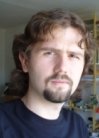
\includegraphics[width=1in,height=1.25in,clip,keepaspectratio]{figures/vitae/bosansky.jpg}
\end{SCfigure}

\begin{SCfigure}[50][h!]
  \caption*{{\bf Viliam Lis{\' y}} is a PhD student and a researcher at Agent Technology Center. He holds master's degree in Technical Artificial Intelligence from VU University Amsterdam and master's degree in Theoretical Computer Science from the Faculty of Mathematics and Physics at Charles University in Prague. Prior to his current position, he worked on automatic emotion recognition at Philips CE Innovation Lab.}
  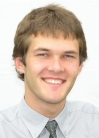
\includegraphics[width=1in,height=1.25in,clip,keepaspectratio]{figures/vitae/lisy.jpg}
\end{SCfigure}

\begin{SCfigure}[50][h!]
  \caption*{{\bf Marc Lanctot} received his Ph.D. degree in Artificial Intelligence from the Department of Computer Science, University of Alberta, Edmonton, Canada,
in 2012. Currently, he is a post-doctoral research fellow at the Department of Knowledge Engineering, Maastricht University. His research interests include 
search and sampling in games.}
  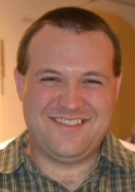
\includegraphics[width=1in,height=1.25in,clip,keepaspectratio]{figures/vitae/marc.jpg}
\end{SCfigure}

\begin{SCfigure}[50][h!]
  \caption*{{\bf Ji{\v r}{\' i} {\v C}erm{\' a}k} is a PhD student at Agent Technology Center, Department of Computer Science, Faculty of Electrical Engineering at Czech Technical University in Prague. His research focuses on computational game theory and sequential games.}
  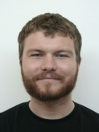
\includegraphics[width=1in,height=1.25in,clip,keepaspectratio]{figures/vitae/cermak.jpg}
\end{SCfigure}

\begin{SCfigure}[50][h!]
  \caption*{{\bf Mark H.M. Winands} received the Ph.D. degree in Artificial Intelligence from the Department of Computer Science, Maastricht University, 
Maastricht, The Netherlands, in 2004. Currently, he is an Assistant Professor at the Department of Knowledge Engineering, Maastricht University. His 
research interests include heuristic search, machine learning and games. Dr. Winands serves as a section editor of the ICGA Journal and as an associate 
editor of IEEE Transactions on Computational Intelligence and AI in Games.}
  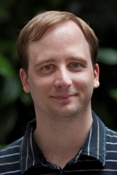
\includegraphics[width=1in,height=1.25in,clip,keepaspectratio]{figures/vitae/mark.jpg} 
\end{SCfigure}








\end{document}

%%
%% End of file `elsarticle-template-1-num.tex'.
